%----------------------------------------------------------------------------------------
%   PACKAGES AND OTHER DOCUMENT CONFIGURATIONS
%----------------------------------------------------------------------------------------
\documentclass[11pt, a4paper,oneside]{book}

\usepackage{graphicx} % Required for including pictures

%----------------------------------------------------------------------------------------
%       Localization
%----------------------------------------------------------------------------------------
\usepackage[UTF8,adobefonts]{ctex}
\usepackage[TS1,T1]{fontenc}
\usepackage{array, booktabs}
\usepackage[x11names]{xcolor}
\usepackage{colortbl}
\usepackage{fontspec}
\newcommand{\foo}{\color{baseD}\makebox[0pt]{\textbullet}\hskip-0.5pt\vrule width 1pt\hspace{\labelsep}}

%\setmainfont[Boldont=WenQuanYi Micro Hei]{AR PL SungtiL GB}
%\setsansfont[BoldFont=WenQuanYi Micro Hei]{AR PL KaitiM GB}
%\setmonofont{DejaVu Sans Mono}

%\XeTeXlinebreaklocale "zh"
%\XeTeXlinebreakskip = 0pt plus 1pt minus 0.1pt

\usepackage[top=1in,bottom=1in,left=1.25in,right=1.25in]{geometry}
%\linespread{1.2}

\usepackage[Glenn]{fncychap}

\usepackage{fancyhdr}

%----------------------------------------------------------------------------------------
%       Useful Packages
%----------------------------------------------------------------------------------------
\usepackage{color}
\usepackage{url}
\usepackage[colorlinks, linkcolor=black,anchorcolor=black, citecolor=black]{hyperref}

\usepackage{xcolor} % Required for specifying colors by name
\definecolor{ocre}{RGB}{243,102,25} % Define the orange color used for highlighting throughout the book

% BASE16
\definecolor{base0}{HTML}{181818}
\definecolor{base1}{HTML}{282828}
\definecolor{base2}{HTML}{383838}
\definecolor{base3}{HTML}{585858}
\definecolor{base4}{HTML}{B8B8B8}
\definecolor{base5}{HTML}{D8D8D8}
\definecolor{base6}{HTML}{E8E8E8}
\definecolor{base7}{HTML}{F8F8F8}
\definecolor{base8}{HTML}{AB4642}
\definecolor{base9}{HTML}{DC9656}
\definecolor{baseA}{HTML}{F7CA88}
\definecolor{baseB}{HTML}{A1B56C}
\definecolor{baseC}{HTML}{86C1B9}
\definecolor{baseD}{HTML}{7CAFC2}
\definecolor{baseE}{HTML}{BA8BAF}
\definecolor{baseF}{HTML}{A16946}
\definecolor{Gray}{HTML}{CCCCCC}
\definecolor{linkcolor}{HTML}{EC008C}
\definecolor{codecolorpink}{HTML}{CC00FF}
\definecolor{NoteColorFont}{HTML}{6D727D}
\definecolor{NoteColorLine}{HTML}{C3CAD9}
\definecolor{ExeColorFont}{HTML}{FF9900}
\definecolor{ExeColorLine}{HTML}{FFF678}
\definecolor{ExeColorBack}{HTML}{FFFFCC}
\definecolor{ThinkColorFont}{HTML}{629D81}
\definecolor{ThinkColorLine}{HTML}{93E87D}
\definecolor{ThinkColorBack}{HTML}{C1FA9B}

\usepackage{amsmath,amsfonts,amssymb,amsthm} % For math equations, theorems, symbols, etc
\usepackage{booktabs} % For tables
\usepackage{tabularx}
\usepackage{multirow} % for multiple row tables.

%----------------------------------------------------------------------------------------
%       Some Extra Definitions
%----------------------------------------------------------------------------------------

\RequirePackage[framemethod=default]{mdframed} % Required for creating the theorem, definition, exercise and corollary boxes

% Exercise box
\newmdenv[skipabove=10pt,
skipbelow=10pt,
rightline=false,
leftline=true,
topline=false,
bottomline=false,
backgroundcolor=ExeColorBack,
linecolor=ExeColorLine,
innerleftmargin=5pt,
innerrightmargin=5pt,
innertopmargin=5pt,
innerbottommargin=5pt,
leftmargin=0cm,
rightmargin=0cm,
linewidth=12pt]{eBox}

% Thinking box
\newmdenv[skipabove=10pt,
skipbelow=10pt,
rightline=false,
leftline=true,
topline=false,
bottomline=false,
backgroundcolor=ThinkColorBack!30,
linecolor=ThinkColorLine,
innerleftmargin=5pt,
innerrightmargin=5pt,
innertopmargin=5pt,
innerbottommargin=5pt,
leftmargin=0cm,
rightmargin=0cm,
linewidth=12pt]{tBox}

% Note box
\newmdenv[skipabove=10pt,
skipbelow=10pt,
rightline=false,
leftline=true,
topline=false,
bottomline=false,
backgroundcolor=NoteColorLine!15,
linecolor=NoteColorLine,
innerleftmargin=5pt,
innerrightmargin=5pt,
innertopmargin=5pt,
innerbottommargin=5pt,
leftmargin=0cm,
rightmargin=0cm,
linewidth=12pt]{nBox}

% Boxed/framed environments
\newtheoremstyle{ocrenumbox}% % Theorem style name
{0pt}% Space above
{0pt}% Space below
{\normalfont}% % Body font
{}% Indent amount
{\small\bf\sffamily\color{ExeColorFont}}% % Theorem head font
{\;}% Punctuation after theorem head
{0.25em}% Space after theorem head  
{\small\sffamily\color{ExeColorFont}\thmname{#1}\nobreakspace\thmnumber{#2}% Theorem text (e.g. Exercise 2.1)
\thmnote{\nobreakspace\the\thm@notefont\sffamily\bfseries\color{black}---\nobreakspace#3.}} % Optional theorem note
\renewcommand{\qedsymbol}{$\blacksquare$}% Optional qed square

\newtheoremstyle{purplenumbox}% % Theorem style name
{0pt}% Space above
{0pt}% Space below
{\normalfont}% % Body font
{}% Indent amount
{\small\bf\sffamily\color{ThinkColorFont}}% % Theorem head font
{\;}% Punctuation after theorem head
{0.25em}% Space after theorem head  
{\small\sffamily\color{ThinkColorFont}\thmname{#1}\nobreakspace\thmnumber{#2}
% Theorem text (e.g. Thinking 2.1)
\thmnote{\nobreakspace\the\thm@notefont\sffamily\bfseries\color{black}---\nobreakspace#3.}} % Optional theorem note
\renewcommand{\qedsymbol}{$\blacksquare$}% Optional qed square

\newtheoremstyle{blackbox} % Theorem style name
{0pt}% Space above
{0pt}% Space below
{\normalfont}% Body font
{}% Indent amount
{\small\bf\sffamily}% Theorem head font
{\;}% Punctuation after theorem head
{0.25em}% Space after theorem head
{\small\sffamily\color{NoteColorFont}\thmname{#1}\nobreakspace\thmnumber{#2}
% Theorem text (e.g. Theorem 2.1)
\thmnote{\nobreakspace\the\thm@notefont\sffamily\bfseries---\nobreakspace#3.}}% Optional theorem note

% Defines the theorem text style for each type of theorem to one of the three styles above
\theoremstyle{ocrenumbox}
\newtheorem{exerciseT}{Exercise}[chapter]
\theoremstyle{purplenumbox}
\newtheorem{thinkingT}{Thinking}[chapter]
\theoremstyle{blackbox}
\newtheorem{noteT}{Note}[section]

\newenvironment{exercise}{\begin{eBox}\begin{exerciseT}}{\hfill{\color{ExeColorFont}\tiny\ensuremath{\blacksquare}}\end{exerciseT}\end{eBox}}
\newenvironment{thinking}{\begin{tBox}\begin{thinkingT}}{\hfill{\color{ThinkColorFont}\tiny\ensuremath{\blacksquare}}\end{thinkingT}\end{tBox}}
\newenvironment{note}{\begin{nBox}\begin{noteT}}{\end{noteT}\end{nBox}}

\usepackage{caption}

\usepackage{minitoc}
\dominitoc[c]
\setcounter{minitocdepth}{4}

%----------------------------------------------------------------------------------------
%       Code Environment
%----------------------------------------------------------------------------------------
\usepackage{minted} 
\usemintedstyle{manni}

% code box
\newmdenv[backgroundcolor=base7,
linecolor=baseD,
bottomline=false,
leftline=true,
rightline=false,
topline=false,
linewidth=2pt,
leftmargin=13pt]{pcodeBox}

\renewcommand{\theFancyVerbLine}{
  \sffamily
  \textcolor{baseB}{\arabic{FancyVerbLine}
  }
}

%\captionsetup{type=codeCaption}
\newenvironment{codeBox}{\begin{pcodeBox}\fontsize{9pt}{9pt}}{\end{pcodeBox}}
\newenvironment{codeBoxWithCaption}[1]{\begin{pcodeBox}[frametitle={\captionof{listing}{#1}\color{base6}\rule{\textwidth}{0.7pt}}]\fontsize{9pt}{9pt}}{\end{pcodeBox}}

\BeforeBeginEnvironment{minted}{\begin{codeBox}}
\AfterEndEnvironment{minted}{\end{codeBox}}

%----------------------------------------------------------------------------------------
%       Lists
%----------------------------------------------------------------------------------------
\usepackage{enumitem}
\setlist[description]{labelindent=22pt} 

%----------------------------------------------------------------------------------------
%       Main Body
%----------------------------------------------------------------------------------------
\begin{document}

\pagestyle{empty} % Removes page numbers
\title{TCP高级实验}
\author{王鹿鸣,刘保证}
\date{\today}
\maketitle
\setcounter{secnumdepth}{3}
\frontmatter
\tableofcontents

\mainmatter
\pagestyle{fancy}

\chapter{准备部分}

\minitoc

\section{用户层TCP}

用户层的TCP编程模型大致如下,对于服务端,调用listen监听端口,
之后接受客户端的请求,然后就可以收发数据了。结束时,关闭socket。

\begin{minted}[linenos]{c}
// Server
socket(...,SOCK_STREAM,0);
bind(...,&server_address, ...);
listen(...);
accept(..., &client_address, ...);
recv(..., &clientaddr, ...);
close(...);
\end{minted}

对于客户端,则调用connect连接服务端,之后便可以收发数据。
最后关闭socket。

\begin{minted}[linenos]{c}
socket(...,SOCK_STREAM,0);
connect();
send(...,&server_address,...);
\end{minted}

那么根据我们的需求,我们着重照顾连接的建立、关闭和封包的收发过程。

\section{探寻tcp\_prot,地图get\textasciitilde{}}

一般游戏的主角手中,都会有一张万能的地图。为了搞定TCP,我们自然也是需要
一张地图的,要不连该去找那个函数看都不知道。很有幸,在\mintinline[linenos]{text}{tcp_ipv4.c}中,
\mintinline[linenos]{text}{tcp_prot}定义了\mintinline[linenos]{text}{tcp}的各个接口。

\mintinline[linenos]{text}{tcp_prot}的类型为\mintinline[linenos]{text}{struct proto},是这个结构体是为了抽象各种不同的协议的
差异性而存在的。类似面向对象中所说的接口(Interface)的概念。这里,我们仅
保留我们关系的部分。

\begin{minted}[linenos]{c}
struct proto tcp_prot = {
        .name                   = "TCP",
        .owner                  = THIS_MODULE,
        .close                  = tcp_close,
        .connect                = tcp_v4_connect,
        .disconnect             = tcp_disconnect,
        .accept                 = inet_csk_accept,
        .destroy                = tcp_v4_destroy_sock,
        .shutdown               = tcp_shutdown,
        .setsockopt             = tcp_setsockopt,
        .getsockopt             = tcp_getsockopt,
        .recvmsg                = tcp_recvmsg,
        .sendmsg                = tcp_sendmsg,
        .sendpage               = tcp_sendpage,
        .backlog_rcv            = tcp_v4_do_rcv,
        .get_port               = inet_csk_get_port,
        .twsk_prot              = &tcp_timewait_sock_ops,
        .rsk_prot               = &tcp_request_sock_ops,
};
\end{minted}

通过名字,我大致筛选出来了这些函数,初步判断这些函数与实验所关心的功能相关。
对着这张``地图'',就可以顺藤摸瓜,找出些路径了。

先根据参考书《Linux内核源码剖析------TCP/IP实现》中给出的流程图,
找出所有和需求相关的部分。

首先找三次握手相关的部分:从客户端的角度,发起连接需要调用\mintinline[linenos]{text}{tcp_v4_connect},
该函数会进一步调用\mintinline[linenos]{text}{tcp_connect},在这个函数中,会调用\mintinline[linenos]{text}{tcp_send_syn_data}
发送SYN报文,并设定超时计时器。第二次握手相关的接收代码在\mintinline[linenos]{text}{tcp_rcv_state_process}中,
该函数实现了除\mintinline[linenos]{text}{ESTABLISHED}和\mintinline[linenos]{text}{TIME_WAIT}之外所有状态下的接收处理。
\mintinline[linenos]{text}{tcp_send_ack}函数实现了发送ACK报文。从服务端的角度,则还需实现\mintinline[linenos]{text}{listen}调用和
\mintinline[linenos]{text}{accept}调用。二者都是服务端建立连接所需要的部分。

封包的封装发送部分,所对应的函数是\mintinline[linenos]{text}{tcp_sendmsg},实现对数据的复制、切割和发送。
TCP的重传接口为\mintinline[linenos]{text}{tcp_retransmit_skb},这里尚有疑问,因为这个函数是负责处理重传的,
而不是判断是否应当重传的。所以并不明确到底是否该重新实现这一部分。

TCP封包的接收在\mintinline[linenos]{text}{tcp_rcv_established}函数中,根据目前有限的资料看,TCP的滑动窗口机制应该
在这一部分,更细节的内容待确认。

\begin{itemize}
\item
  tcp\_transmit\_skb
\item
  tcp\_rcv\_state\_process
\item
  tcp\_connect
\item
  tcp\_rcv\_synsent\_state\_process
\item
  tcp\_rcv\_established
\item
  tcp\_send\_ack
\item
  tcp\_sendmsg
\item
  tcp\_retransmit\_skb
\item
  tcp\_rcv\_established
\end{itemize}

\section{RFC}
\label{sec:rfc}

在分析TCP的过程中会遇到很多RFC,在这里,我们将可能会碰到的RFC罗列出来。
并进行一定的讨论。便于后面的分析。

\subsection{RFC793——Transmission Control Protocol}
\label{subsec:rfc793}

该RFC正是定义了TCP协议的那份RFC。在该RFC中,可以查到TCP的很多细节,帮助后续的代码分析。

\subsubsection{TCP头部格式}
\label{subsubsec:tcp_header_format}
RFC793中,对于TCP头部格式的描述摘录如下:
\begin{minted}[linenos]{text}
    0                   1                   2                   3   
    0 1 2 3 4 5 6 7 8 9 0 1 2 3 4 5 6 7 8 9 0 1 2 3 4 5 6 7 8 9 0 1 
   +-+-+-+-+-+-+-+-+-+-+-+-+-+-+-+-+-+-+-+-+-+-+-+-+-+-+-+-+-+-+-+-+
   |          Source Port          |       Destination Port        |
   +-+-+-+-+-+-+-+-+-+-+-+-+-+-+-+-+-+-+-+-+-+-+-+-+-+-+-+-+-+-+-+-+
   |                        Sequence Number                        |
   +-+-+-+-+-+-+-+-+-+-+-+-+-+-+-+-+-+-+-+-+-+-+-+-+-+-+-+-+-+-+-+-+
   |                    Acknowledgment Number                      |
   +-+-+-+-+-+-+-+-+-+-+-+-+-+-+-+-+-+-+-+-+-+-+-+-+-+-+-+-+-+-+-+-+
   |  Data |           |U|A|P|R|S|F|                               |
   | Offset| Reserved  |R|C|S|S|Y|I|            Window             |
   |       |           |G|K|H|T|N|N|                               |
   +-+-+-+-+-+-+-+-+-+-+-+-+-+-+-+-+-+-+-+-+-+-+-+-+-+-+-+-+-+-+-+-+
   |           Checksum            |         Urgent Pointer        |
   +-+-+-+-+-+-+-+-+-+-+-+-+-+-+-+-+-+-+-+-+-+-+-+-+-+-+-+-+-+-+-+-+
   |                    Options                    |    Padding    |
   +-+-+-+-+-+-+-+-+-+-+-+-+-+-+-+-+-+-+-+-+-+-+-+-+-+-+-+-+-+-+-+-+
   |                             data                              |
   +-+-+-+-+-+-+-+-+-+-+-+-+-+-+-+-+-+-+-+-+-+-+-+-+-+-+-+-+-+-+-+-+

                            TCP Header Format

          Note that one tick mark represents one bit position.
\end{minted}
这张图可以很方便地读出各个位占多长,它上面的标识是十进制的,很容易读。
这里我们挑出我们比较关心的Options字段来解读。因为很多TCP的扩展都是通过新增
选项来实现的。

选项总是在TCP头部的最后,且选项有两种格式:
\begin{enumerate}
\item 单独的一个字节,代表选项的类型例如:

\begin{minted}[linenos]{text}
  End of Option List
  +--------+
  |00000000| 
  +--------+ 
  Kind=0
\end{minted}

\item 第一个字节代表选项的类型,紧跟着的一个字节代表选项的长度,后面跟着
选项的数据。例如:

\begin{minted}[linenos]{text}
  Maximum Segment Size
  +--------+--------+---------+--------+ 
  |00000010|00000100| max seg size     | 
  +--------+--------+---------+--------+ 
    Kind=2  Length=4
\end{minted}

\end{enumerate}

\subsection{RFC1323——TCP Extensions for High Performance}
\label{subsec:rfc1323}

\subsubsection{简介}
\label{subsubsec:rfc1323_introduce}
这个RFC主要是在考虑高带宽高延迟网络下如何提升TCP的性能。该RFC定义了新的TCP选项,
以实现窗口缩放(window scaled)和时间戳(timestamp)。这里的时间戳可以用于实现
两个机制:RTTM(Round Trip Time Measurement)和PAWS(Protect Against Wrapped Sequences)。

在RFC1323中提出,在这类高带宽高延迟网络下,有三个主要的影响TCP性能的因素:
\begin{description}
  \item[窗口尺寸限制] 在TCP头部中,只有16位的一个域用于说明窗口大小。也就是说,
    窗口大小最大只能达到$2^{16}=64K字节$。解决这一问题的方案是增加一个窗口缩放
    选项,我们会在\ref{subsubsec:window_scale}中进一步讨论。
  \item[丢包后的恢复] 丢包会导致TCP重新进入慢启动状态,导致数据的流水线断流。
    在引入了快重传和快恢复后,可以解决丢包率为一个窗口中丢一个包的情况下的问题。
    但是在引入了窗口缩放以后,由于窗口的扩大,丢包的概率也随之增加。很容易使TCP进入
    到慢启动状态,影响网络性能。为了解决这一问题,需要引入SACK机制,但在这个RFC中,
    不讨论SACK相关的问题。
  \item[往返时间度量] RTO(Retransmission timeout)是TCP性能的一个很基础的参数。
    在RFC1323中介绍了一种名为RTTM的机制,利用一个新的名为Timestamps的选项来对时间
    进行进一步的统计。
\end{description}

\subsubsection{窗口缩放(Window Scale)}
\label{subsubsec:window_scale}
这一扩展将原有的TCP窗口扩展到32位。而根据RFC793中的定义,TCP头部描述窗口大小的域仅有16位。
为了将其扩展为32位,该扩展定义了一个新的选项用于表示缩放因子。这一选项仅会出现在SYN段,
此后,所有通过该连接的通信,其窗口大小都会受到这一选项的影响。

该选项的格式为:
\begin{minted}[linenos]{text}
  +---------+---------+---------+ 
  | Kind=3  |Length=3 |shift.cnt| 
  +---------+---------+---------+
\end{minted}

\mintinline{text}{kind}域为3,\mintinline{text}{length}域为3,后面跟着3个字节的
\mintinline{text}{shift.cnt},代表缩放因子。TCP的Options域的选项的格式在
\ref{subsubsec:tcp_header_format}中已有说明。这里采用的是第二种格式。

在启用了窗口缩放以后,TCP头部中的接收窗口大小,就变为了真实的接收窗口大小右移
\mintinline{text}{shift.cnt}的值。RFC中对于该选项的实现的建议是在传输控制块中,
按照32位整型来存储所有的窗口值,包括发送窗口、接受窗口和拥塞窗口。

作为接收方,每当收到一个段时(除SYN段外),通过将发来的窗口值左移来得到正确的值。
\begin{minted}[linenos]{c}
SND.WND = SEG.WND << Snd.Wind.Scale
\end{minted}

作为发送方则每次在发包前,将发送窗口的值右移,然后再封装在封包中。
\begin{minted}[linenos]{c}
SEG.WND = RCV.WND >> Rcv.Wind.Scale
\end{minted}

\subsubsection{PAWS(Protect Against Wrapped Sequence Numbers)}
PAWS是一个用于防止旧的重复封包带来的问题的机制。它采用了TCP中的Timestamps选项。
该选项的格式为:
\begin{minted}[linenos]{text}
+-------+-------+---------------------+---------------------+ 
|Kind=8 |  10   |   TS Value (TSval)  |TS Echo Reply (TSecr)| 
+-------+-------+---------------------+---------------------+
    1       1              4                      4
\end{minted}
TSval(Timestamp Value)包含了TCP发送方的时钟的当前值。如果ACK位被设置了的话,
TSecr(Timestamp Echo Reply)会包含一个由对方发送过来的最近的时钟值。

PAWS的算法流程为:
\begin{enumerate}
  \item 如果当前到达的段SEG含有Timestamps选项,且SEG.TSval < TS.Recent且
该TS.Recent是有效的,那么则认为当前到达的分段是不可被接受的,需要丢弃掉。
  \item 如果段超过了窗口的范围,则丢弃它(与正常的TCP处理相同)
  \item 如果满足SEG.SEQ$\leqslant$Last.ACK.sent(最后回复的ACK包中的时间戳),
    那么,将SEG的时间戳记录为TS.Recent。
  \item 如果SEG是正常按顺序到达的,那么正常地接收它。
  \item 其他情况下,将该段视作正常的在窗口中,但顺序不正确的TCP段对待。
\end{enumerate}

\subsection{RFC3168}
\label{subsec:rfc3168}


\chapter{网络子系统相关核心数据结构}
\minitoc
    \section{网络子系统数据结构架构}    
%----------------------------------------------------------------------------------------
%                   Structure about Sock
%----------------------------------------------------------------------------------------
    \section{sock底层数据结构}  
        \subsection{sock\_common}

\begin{minted}[linenos]{C}
/*
Location:

	include/net/sock.h

Description:

	minimal network layer representation of sockets
	This is the minimal network layer representation of sockets, the header
	for struct sock and struct inet_timewait_sock.
Member:

 *  @skc_daddr: Foreign IPv4 addr
 *  @skc_rcv_saddr: Bound local IPv4 addr
 *  @skc_hash: hash value used with various protocol lookup tables
 *  @skc_u16hashes: two u16 hash values used by UDP lookup tables
 *  @skc_dport: placeholder for inet_dport/tw_dport
 *  @skc_num: placeholder for inet_num/tw_num
 *  @skc_family: network address family
 *  @skc_state: Connection state
 *  @skc_reuse: %SO_REUSEADDR setting
 *  @skc_reuseport: %SO_REUSEPORT setting
 *  @skc_bound_dev_if: bound device index if != 0
 *  @skc_bind_node: bind hash linkage for various protocol lookup tables
 *  @skc_portaddr_node: second hash linkage for UDP/UDP-Lite protocol
 *  @skc_prot: protocol handlers inside a network family
 *  @skc_net: reference to the network namespace of this socket
 *  @skc_node: main hash linkage for various protocol lookup tables
 *  @skc_nulls_node: main hash linkage for TCP/UDP/UDP-Lite protocol
 *  @skc_tx_queue_mapping: tx queue number for this connection
 *  @skc_flags: place holder for sk_flags
 *      %SO_LINGER (l_onoff), %SO_BROADCAST, %SO_KEEPALIVE,
 *      %SO_OOBINLINE settings, %SO_TIMESTAMPING settings
 *  @skc_incoming_cpu: record/match cpu processing incoming packets
 *  @skc_refcnt: reference count
*/
struct sock_common {
    /* skc_daddr and skc_rcv_saddr must be grouped on a 8 bytes aligned
     * address on 64bit arches : cf INET_MATCH()
     */
    union {
        __addrpair  skc_addrpair;
        struct {
            __be32  skc_daddr;
            __be32  skc_rcv_saddr;
        };
    };
    union  {
        unsigned int    skc_hash;
        __u16       skc_u16hashes[2];
    };
    /* skc_dport && skc_num must be grouped as well */
    union {
        __portpair  skc_portpair;
        struct {
            __be16  skc_dport;
            __u16   skc_num;
        };
    };

    unsigned short      skc_family;
    volatile unsigned char  skc_state;
    unsigned char       skc_reuse:4;
    unsigned char       skc_reuseport:1;
    unsigned char       skc_ipv6only:1;
    unsigned char       skc_net_refcnt:1;
    int         skc_bound_dev_if;
    union {
        struct hlist_node   skc_bind_node;
        struct hlist_nulls_node skc_portaddr_node;
    };
    struct proto        *skc_prot;
    possible_net_t      skc_net;

#if IS_ENABLED(CONFIG_IPV6)
    struct in6_addr     skc_v6_daddr;
    struct in6_addr     skc_v6_rcv_saddr;
#endif

    atomic64_t      skc_cookie;

    /* following fields are padding to force
     * offset(struct sock, sk_refcnt) == 128 on 64bit arches
     * assuming IPV6 is enabled. We use this padding differently
     * for different kind of 'sockets'
     */
    union {
        unsigned long   skc_flags;
        struct sock *skc_listener; /* request_sock */
        struct inet_timewait_death_row *skc_tw_dr; /* inet_timewait_sock */
    };
    /*
     * fields between dontcopy_begin/dontcopy_end
     * are not copied in sock_copy()
     */
    /* private: */
    int         skc_dontcopy_begin[0];
    /* public: */
    union {
        struct hlist_node   skc_node;
        struct hlist_nulls_node skc_nulls_node;
    };
    int         skc_tx_queue_mapping;
    union {
        int     skc_incoming_cpu;
        u32     skc_rcv_wnd;
        u32     skc_tw_rcv_nxt; /* struct tcp_timewait_sock  */
    };

    atomic_t        skc_refcnt;
    /* private: */
    int                     skc_dontcopy_end[0];
    union {
        u32     skc_rxhash;
        u32     skc_window_clamp;
        u32     skc_tw_snd_nxt; /* struct tcp_timewait_sock */
    };
    /* public: */
};
\end{minted}
        \subsection{sock}
\begin{minted}[linenos]{C}
/*
Location:

	include/net/sock.h

Description:

	sock结构是比较通用的网络层描述块,构成传输控制块的基础,与具体的协议族无关。
	它描述了各协议族的公共信息,因此不能直接作为传输层控制块来使用。不同协议族的
	传输层在使用该结构的时候都会对其进行拓展,来适合各自的传输特性。例如,inet_sock
	结构由sock结构及其它特性组成,构成了IPV4协议族传输控制块的基础。

Member:
  * struct sock - network layer representation of sockets
  * @__sk_common: shared layout with inet_timewait_sock
  * @sk_shutdown: SEND_SHUTDOWN 或者 RCV_SHUTDOWN的掩码
  * @sk_userlocks: %SO_SNDBUF and %SO_RCVBUF settings
  * @sk_lock:   synchronizer
  * @sk_rcvbuf: 接受缓冲区的大小(单位为字节)
  * @sk_wq: sock wait queue and async head
  * @sk_rx_dst: receive input route used by early demux
  * @sk_dst_cache: destination cache
  * @sk_policy: flow policy
  * @sk_receive_queue: incoming packets
  * @sk_wmem_alloc: transmit queue bytes committed
  * @sk_write_queue: Packet sending queue
  * @sk_omem_alloc: "o" is "option" or "other"
  * @sk_wmem_queued: persistent queue size
  * @sk_forward_alloc: space allocated forward
  * @sk_napi_id: id of the last napi context to receive data for sk
  * @sk_ll_usec: usecs to busypoll when there is no data
  * @sk_allocation: allocation mode
  * @sk_pacing_rate: Pacing rate (if supported by transport/packet scheduler)
  * @sk_max_pacing_rate: Maximum pacing rate (%SO_MAX_PACING_RATE)
  * @sk_sndbuf: size of send buffer in bytes
  * @sk_no_check_tx: %SO_NO_CHECK setting, set checksum in TX packets
  * @sk_no_check_rx: allow zero checksum in RX packets
  * @sk_route_caps: route capabilities (e.g. %NETIF_F_TSO)
  * @sk_route_nocaps: forbidden route capabilities (e.g NETIF_F_GSO_MASK)
  * @sk_gso_type: GSO type (e.g. %SKB_GSO_TCPV4)
  * @sk_gso_max_size: Maximum GSO segment size to build
  * @sk_gso_max_segs: Maximum number of GSO segments
  * @sk_lingertime: %SO_LINGER l_linger setting
  * @sk_backlog: always used with the per-socket spinlock held
  * @sk_callback_lock: used with the callbacks in the end of this struct
  * @sk_error_queue: rarely used
  * @sk_prot_creator: sk_prot of original sock creator (see ipv6_setsockopt,
  *           IPV6_ADDRFORM for instance)
  * @sk_err: last error
  * @sk_err_soft: errors that don't cause failure but are the cause of a
  *           persistent failure not just 'timed out'
  * @sk_drops: raw/udp drops counter
  * @sk_ack_backlog: current listen backlog
  * @sk_max_ack_backlog: listen backlog set in listen()
  * @sk_priority: %SO_PRIORITY setting
  * @sk_cgrp_prioidx: socket group's priority map index
  * @sk_type: socket type (%SOCK_STREAM, etc)
  * @sk_protocol: which protocol this socket belongs in this network family
  * @sk_peer_pid: &struct pid for this socket's peer
  * @sk_peer_cred: %SO_PEERCRED setting
  * @sk_rcvlowat: %SO_RCVLOWAT setting
  * @sk_rcvtimeo: %SO_RCVTIMEO setting
  * @sk_sndtimeo: %SO_SNDTIMEO setting
  * @sk_txhash: computed flow hash for use on transmit
  * @sk_filter: socket filtering instructions
  * @sk_timer: sock cleanup timer
  * @sk_stamp: time stamp of last packet received
  * @sk_tsflags: SO_TIMESTAMPING socket options
  * @sk_tskey: counter to disambiguate concurrent tstamp requests
  * @sk_socket: Identd and reporting IO signals
  * @sk_user_data: RPC layer private data
  * @sk_frag: cached page frag
  * @sk_peek_off: current peek_offset value
  * @sk_send_head: 发送队列的头指针
  * @sk_security: used by security modules
  * @sk_mark: generic packet mark
  * @sk_classid: this socket's cgroup classid
  * @sk_cgrp: this socket's cgroup-specific proto data
  * @sk_write_pending: a write to stream socket waits to start
  * @sk_state_change: callback to indicate change in the state of the sock
  * @sk_data_ready: callback to indicate there is data to be processed
  * @sk_write_space: callback to indicate there is bf sending space available
  * @sk_error_report: callback to indicate errors (e.g. %MSG_ERRQUEUE)
  * @sk_backlog_rcv: callback to process the backlog
  * @sk_destruct: called at sock freeing time, i.e. when all refcnt == 0
 */
struct sock {
    /*
     * Now struct inet_timewait_sock also uses sock_common, so please just
     * don't add nothing before this first member (__sk_common) --acme
     */
    struct sock_common  __sk_common;
#define sk_node         __sk_common.skc_node
#define sk_nulls_node       __sk_common.skc_nulls_node
#define sk_refcnt       __sk_common.skc_refcnt
#define sk_tx_queue_mapping __sk_common.skc_tx_queue_mapping

#define sk_dontcopy_begin   __sk_common.skc_dontcopy_begin
#define sk_dontcopy_end     __sk_common.skc_dontcopy_end
#define sk_hash         __sk_common.skc_hash
#define sk_portpair     __sk_common.skc_portpair
#define sk_num          __sk_common.skc_num
#define sk_dport        __sk_common.skc_dport
#define sk_addrpair     __sk_common.skc_addrpair
#define sk_daddr        __sk_common.skc_daddr
#define sk_rcv_saddr        __sk_common.skc_rcv_saddr
#define sk_family       __sk_common.skc_family
#define sk_state        __sk_common.skc_state
#define sk_reuse        __sk_common.skc_reuse
#define sk_reuseport        __sk_common.skc_reuseport
#define sk_ipv6only     __sk_common.skc_ipv6only
#define sk_net_refcnt       __sk_common.skc_net_refcnt
#define sk_bound_dev_if     __sk_common.skc_bound_dev_if
#define sk_bind_node        __sk_common.skc_bind_node
#define sk_prot         __sk_common.skc_prot
#define sk_net          __sk_common.skc_net
#define sk_v6_daddr     __sk_common.skc_v6_daddr
#define sk_v6_rcv_saddr __sk_common.skc_v6_rcv_saddr
#define sk_cookie       __sk_common.skc_cookie
#define sk_incoming_cpu     __sk_common.skc_incoming_cpu
#define sk_flags        __sk_common.skc_flags
#define sk_rxhash       __sk_common.skc_rxhash

    socket_lock_t       sk_lock;
    struct sk_buff_head sk_receive_queue;
    /*
     * The backlog queue is special, it is always used with
     * the per-socket spinlock held and requires low latency
     * access. Therefore we special case it's implementation.
     * Note : rmem_alloc is in this structure to fill a hole
     * on 64bit arches, not because its logically part of
     * backlog.
     */
    struct {
        atomic_t    rmem_alloc;
        int     len;
        struct sk_buff  *head;
        struct sk_buff  *tail;
    } sk_backlog;
#define sk_rmem_alloc sk_backlog.rmem_alloc
    int         sk_forward_alloc;

    __u32           sk_txhash;
#ifdef CONFIG_NET_RX_BUSY_POLL
    unsigned int        sk_napi_id;
    unsigned int        sk_ll_usec;
#endif
    atomic_t        sk_drops;
    int         sk_rcvbuf;

    struct sk_filter __rcu  *sk_filter;
    union {
        struct socket_wq __rcu  *sk_wq;
        struct socket_wq    *sk_wq_raw;
    };
#ifdef CONFIG_XFRM
    struct xfrm_policy __rcu *sk_policy[2];
#endif
    struct dst_entry    *sk_rx_dst;
    struct dst_entry __rcu  *sk_dst_cache;
    /* Note: 32bit hole on 64bit arches */
    atomic_t        sk_wmem_alloc;
    atomic_t        sk_omem_alloc;
    int         sk_sndbuf;
    struct sk_buff_head sk_write_queue;
    kmemcheck_bitfield_begin(flags);
    unsigned int        sk_shutdown  : 2,
                sk_no_check_tx : 1,
                sk_no_check_rx : 1,
                sk_userlocks : 4,
                sk_protocol  : 8,
                sk_type      : 16;
#define SK_PROTOCOL_MAX U8_MAX
    kmemcheck_bitfield_end(flags);
    int         sk_wmem_queued;
    gfp_t           sk_allocation;
    u32         sk_pacing_rate; /* bytes per second */
    u32         sk_max_pacing_rate;
    netdev_features_t   sk_route_caps;
    netdev_features_t   sk_route_nocaps;
    int         sk_gso_type;
    unsigned int        sk_gso_max_size;
    u16         sk_gso_max_segs;
    int         sk_rcvlowat;
    unsigned long           sk_lingertime;
    struct sk_buff_head sk_error_queue;
    struct proto        *sk_prot_creator;
    rwlock_t        sk_callback_lock;
    int         sk_err,
                sk_err_soft;
    u32         sk_ack_backlog;
    u32         sk_max_ack_backlog;
    __u32           sk_priority;
#if IS_ENABLED(CONFIG_CGROUP_NET_PRIO)
    __u32           sk_cgrp_prioidx;
#endif
    struct pid      *sk_peer_pid;
    const struct cred   *sk_peer_cred;
    long            sk_rcvtimeo;
    long            sk_sndtimeo;
    struct timer_list   sk_timer;
    ktime_t         sk_stamp;
    u16         sk_tsflags;
    u32         sk_tskey;
    struct socket       *sk_socket;
    void            *sk_user_data;
    struct page_frag    sk_frag;
    struct sk_buff      *sk_send_head;
    __s32           sk_peek_off;
    int         sk_write_pending;
#ifdef CONFIG_SECURITY
    void            *sk_security;
#endif
    __u32           sk_mark;
#ifdef CONFIG_CGROUP_NET_CLASSID
    u32         sk_classid;
#endif
    struct cg_proto     *sk_cgrp;
    void            (*sk_state_change)(struct sock *sk);
    void            (*sk_data_ready)(struct sock *sk);
    void            (*sk_write_space)(struct sock *sk);
    void            (*sk_error_report)(struct sock *sk);
    int         (*sk_backlog_rcv)(struct sock *sk,
                          struct sk_buff *skb);
    void                    (*sk_destruct)(struct sock *sk);
};
\end{minted}
    \subsection{\mintinline{C}{request_sock}}

\begin{minted}[linenos]{C}
/* 
Location:

	/include/net/request_sock.h

Description:
	
	struct request_sock - mini sock to represent a connection request
	该结构用于表示一个简单的TCP连接请求。
*/
struct request_sock {
    struct sock_common      __req_common;
#define rsk_refcnt          __req_common.skc_refcnt
#define rsk_hash            __req_common.skc_hash
#define rsk_listener            __req_common.skc_listener
#define rsk_window_clamp        __req_common.skc_window_clamp
#define rsk_rcv_wnd         __req_common.skc_rcv_wnd

    struct request_sock     *dl_next;
    u16             mss;
    u8              num_retrans; /* number of retransmits */
    u8              cookie_ts:1; /* syncookie: encode tcpopts in timestamp */
    u8              num_timeout:7; /* number of timeouts */
    u32             ts_recent;
    struct timer_list       rsk_timer;
    const struct request_sock_ops   *rsk_ops;
    struct sock         *sk;
    u32             *saved_syn;
    u32             secid;
    u32             peer_secid;
};
\end{minted}

    \subsection{sk\_buff}
\label{sec:sk_buff}

\mintinline{c}{struct sk_buff}这一结构体在各层协议中都会被用到。该结构体存储了
网络数据报的所有信息。包括各层的头部以及payload,以及必要的各层实现相关的信息。

该结构体的定义较长,需要一点一点分析。结构体的开头为
\begin{minted}[linenos]{c}
  union {
    struct {
      /* These two members must be first. */
      struct sk_buff          *next;
      struct sk_buff          *prev;

      union {
        ktime_t         tstamp;
        struct skb_mstamp skb_mstamp;
      };
    };
    struct rb_node  rbnode; /* used in netem and tcp stack */
  };
\end{minted}

可以看到,\mintinline{c}{sk_buff}可以被组织成两种数据结构:
双向链表和红黑树。且一个\mintinline{c}{sk_buff}不是在双向链表中,就是在
红黑树中,因此,采用了union来节约空间。next和prev两个域是用于双向链表的结构体,
而rbnode是红黑树相关的结构。

包的到达/发送时间存放在\mintinline{c}{union {ktime_t tstamp;struct skb_mstamp skb_mstamp;};}中,
之所以这里有两种不同的时间戳类型,是因为有时候调用\mintinline{c}{ktime_get()}的
成本太高。因此,内核开发者希望能够在TCP协议栈中实现一个轻量级的微秒级的时间戳。
\mintinline{c}{struct skb_mstamp}正是结合了\mintinline{c}{local_clock()}和
\mintinline{c}{jiffies}二者,而实现的一个轻量级的工具。当然,根据内核邮件列表中
的说法,并不是任何时候都可以用该工具替换调\mintinline{c}{ktime_get()}的。
因此,在\mintinline{c}{struct sk_buff}结构体中,采用\mintinline{c}{union}的方式
同时保留了这二者。

在定义完数据结构相关的一些部分后,又定义了如下的结构体
\begin{minted}[linenos]{c}
  /* 拥有该sk_buff的套接字的指针 */
  struct sock             *sk;
  /* 与该包关联的网络设备 */
  struct net_device       *dev;
  /* 控制用的缓冲区,用于存放各层的私有数据 */
  char                    cb[48] __aligned(8);
  /* 存放了目的地项的引用计数 */
  unsigned long           _skb_refdst;
  /* 析构函数 */
  void                    (*destructor)(struct sk_buff *skb);
#ifdef CONFIG_XFRM
  /* xfrm加密通道 */
  struct  sec_path        *sp;
#endif
#if IS_ENABLED(CONFIG_BRIDGE_NETFILTER)
  /* 保存和bridge相关的信息 */
  struct nf_bridge_info   *nf_bridge;
#endif
\end{minted}

其中的\mintinline{c}{char cb[48]}比较有意思,各层都使用这个buffer来存放自己
私有的变量。这里值得注意的是,如果想要跨层传递数据,则需要使用
\mintinline{c}{skb_clone()}。XFRM则是Linux在2.6版本中引入的一个安全方面的扩展。

之后,又定义了一些长度相关的字段。\mintinline{c}{len}代表buffer中的数据报总长度(含
各协议的头部),以及分片长度。而\mintinline{c}{data_len}代表分片中的数据的长度。
\mintinline{c}{mac_len}是MAC层头部的长度。\mintinline{c}{hdr_len}是一个
克隆出来的可写的头部的长度。
\begin{minted}[linenos]{c}
unsigned int            len,
                        data_len;
__u16                   mac_len,
                        hdr_len;
\end{minted}

kmemcheck是内核中的一套内存检测工具。kmemcheck\_bitfield\_begin
和kmemcheck\_bitfield\_end可以用于说明一段内容的起始和终止位置。
其代码定义如下:
\begin{minted}[linenos]{c}
#define kmemcheck_bitfield_begin(name)  \
        int name##_begin[0];

#define kmemcheck_bitfield_end(name)    \
        int name##_end[0];
\end{minted}

通过定义,我们不难看出,这两个宏是用于在代码中产生两个对应于位域的起始地址和终止地址的
符号的。当然,这两个宏是为kmemcheck的功能服务的。如果没有开启该功能的话,这两个宏的
定义为空,也即不会产生任何作用。
\begin{minted}[linenos]{c}
/* Following fields are _not_ copied in __copy_skb_header()
* Note that queue_mapping is here mostly to fill a hole.
*/
kmemcheck_bitfield_begin(flags1);
__u16       queue_mapping;      /* 对于多队列设备的队列关系映射                 */
__u8        cloned:1,           /* 是否被克隆                               */
            nohdr:1,            /* 只引用了负载                                 */
            fclone:2,           /* skbuff克隆的情况                             */
            peeked:1,           /* peeked表明该包已经被统计过了,无需再次统计 */
            head_frag:1,
            xmit_more:1;        /* 在队列中有更多的SKB在等待                    */
/* one bit hole */
kmemcheck_bitfield_end(flags1);
\end{minted}

在这段定义中,内核将一系列的标志位命名为了flags1,利用那两个函数可以在生成的代码中插入
\mintinline{c}{flags1_begin}和\mintinline{c}{flags1_end}两个符号。这样,当有需要
的时候,可以通过这两个符号找到这一段的起始地址和结束地址。

紧接着是一个包的头部,这一部分再次使用了类似上面的方法,用了两个零长度的数组
\mintinline{c}{headers_start}和\mintinline{c}{headers_end}来标明头部的起始
和终止地址。
\begin{minted}[linenos]{c}
        /* 在__copy_skb_header()中,只需使用一个memcpy()即可将headers_start/end
         * 之间的部分克隆一份。
         */
        /* private: */
        __u32                   headers_start[0];
        /* public: */

/* if you move pkt_type around you also must adapt those constants */
#ifdef __BIG_ENDIAN_BITFIELD
#define PKT_TYPE_MAX    (7 << 5)
#else
#define PKT_TYPE_MAX    7
#endif
#define PKT_TYPE_OFFSET()       offsetof(struct sk_buff, __pkt_type_offset)

        __u8                    __pkt_type_offset[0];
        /* 该包的类型 */
        __u8                    pkt_type:3;
        __u8                    pfmemalloc:1;
        /* 是否允许本地分片(local fragmentation) */
        __u8                    ignore_df:1; 
        /* 表明该skb和连接的关系 */
        __u8                    nfctinfo:3;
        /* netfilter包追踪标记 */
        __u8                    nf_trace:1;
        /* 驱动(硬件)给出来的checksum */
        __u8                    ip_summed:2;
        /* 允许该socket到队列的对应关系发生变更 */
        __u8                    ooo_okay:1;
        /* 表明哈希值字段hash是一个典型的4元组的通过传输端口的哈希 */
        __u8                    l4_hash:1;
        /* 表明哈希值字段hash是通过软件栈计算出来的 */
        __u8                    sw_hash:1;
        /* 表明wifi_acked是否被设置了 */
        __u8                    wifi_acked_valid:1;
        /* 表明帧是否在wifi上被确认了 */
        __u8                    wifi_acked:1;
        
        /* 请求NIC将最后的4个字节作为以太网FCS来对待 */
        __u8                    no_fcs:1;
        /* Indicates the inner headers are valid in the skbuff. */
        __u8                    encapsulation:1;
        __u8                    encap_hdr_csum:1;
        __u8                    csum_valid:1;
        __u8                    csum_complete_sw:1;
        __u8                    csum_level:2;
        __u8                    csum_bad:1;

#ifdef CONFIG_IPV6_NDISC_NODETYPE
        __u8                    ndisc_nodetype:2; /* 路由类型(来自链路层) */
#endif
        /* 标明该skbuff是否被ipvs拥有 */
        __u8                    ipvs_property:1;
        __u8                    inner_protocol_type:1;
        __u8                    remcsum_offload:1;
        /* 3 or 5 bit hole */

#ifdef CONFIG_NET_SCHED
        __u16                   tc_index;       /* traffic control index */
#ifdef CONFIG_NET_CLS_ACT
        __u16                   tc_verd;        /* traffic control verdict */
#endif
#endif

        union {
                __wsum          csum; /* 校验码 */
                struct {
                        /* 从skb->head开始到应当计算校验码的起始位置的偏移 */
                        __u16   csum_start; 
                        /* 从csum_start开始到存储校验码的位置的偏移 */
                        __u16   csum_offset;
                };
        };
        __u32                   priority; /* 包队列的优先级 */
        int                     skb_iif; /* 到达的设备的序号 */
        __u32                   hash; /* 包的哈希值 */
        __be16                  vlan_proto; /* vlan包装协议 */
        __u16                   vlan_tci; /* vlan tag控制信息 */
#if defined(CONFIG_NET_RX_BUSY_POLL) || defined(CONFIG_XPS)
        union {
                unsigned int    napi_id; /* 表明该skb来源的NAPI结构体的id */
                unsigned int    sender_cpu;
        };
#endif
        union {
#ifdef CONFIG_NETWORK_SECMARK
                __u32           secmark; /* 安全标记 */
#endif
#ifdef CONFIG_NET_SWITCHDEV
                __u32           offload_fwd_mark; /* fwding offload mark */
#endif
        };

        union {
                __u32           mark; /* 通用的包的标记位 */
                __u32           reserved_tailroom;
        };

        union {
                __be16          inner_protocol; /* 协议(封装好的) */
                __u8            inner_ipproto;
        };

        /* 已封装的内部传输层头部 */
        __u16                   inner_transport_header; 
        /* 已封装的内部网络层头部 */
        __u16                   inner_network_header; 
        /* 已封装的内部链路层头部 */
        __u16                   inner_mac_header;

        /* 驱动(硬件)给出的包的协议类型 */
        __be16                  protocol;
        /* 传输层头部 */
        __u16                   transport_header;
        /* 网络层头部 */
        __u16                   network_header;
        /* 数据链路层头部 */
        __u16                   mac_header;

        /* private: */
        __u32                   headers_end[0];
\end{minted}

最后是一组是管理相关的字段。其中,\mintinline{c}{head}和\mintinline{c}{end}
代表被分配的内存的起始位置和终止位置。而\mintinline{c}{data}和\mintinline{c}{tail}
则是实际数据的起始和终止位置。
\begin{minted}[linenos]{c}
/* These elements must be at the end, see alloc_skb() for details.  */
        sk_buff_data_t          tail;
        sk_buff_data_t          end;
        unsigned char           *head,
                                *data;
        unsigned int            truesize;
        atomic_t                users;
\end{minted}
\mintinline{c}{users}是引用计数,所以是个原子的。\mintinline{c}{truesize}是
数据报的真实大小。

\subsection{msghdr}
\begin{minted}[linenos]{c}
/* Location: include/linux/socket.h */
struct msghdr {
        void            *msg_name;      /* 指向socket地址结构体的指针 */
        int             msg_namelen;    /* socket地址结构体的大小 */
        struct iov_iter msg_iter;       /* 数据 */
        void            *msg_control;   /* 辅助数据 */
        __kernel_size_t msg_controllen; /* 辅助数据缓冲区大小 */
        unsigned int    msg_flags;      /* 收到的消息所带的标记 */
        struct kiocb    *msg_iocb;      /* 指向iocb的指针(用于异步请求) */
};
\end{minted}

%----------------------------------------------------------------------------------------
%                   Structure about Inet
%----------------------------------------------------------------------------------------
    \section{inet层相关数据结构}
        \subsection{\mintinline{C}{ip_options}}

\begin{minted}[linenos]{C}


/*
Location:

Description:
    @faddr - Saved first hop address
    @nexthop - Saved nexthop address in LSRR and SSRR
    @is_strictroute - Strict source route
    @srr_is_hit - Packet destination addr was our one
    @is_changed - IP checksum more not valid
    @rr_needaddr - Need to record addr of outgoing dev
    @ts_needtime - Need to record timestamp
    @ts_needaddr - Need to record addr of outgoing dev
*/
struct ip_options {
    __be32      faddr;
	/*下一跳*/
    __be32      nexthop;
	/*标识IP首部中选项所占的字节数*/
    unsigned char   optlen;
	/*
		记录宽松路由或严格路由选项在IP首部中的偏移量,
		即选项的第一个字节的地址减去IP首部的第一个字节的地址
	*/
    unsigned char   srr;
    unsigned char   rr;
    unsigned char   ts;
    unsigned char   is_strictroute:1,
            srr_is_hit:1,
            is_changed:1,
            rr_needaddr:1,
            ts_needtime:1,
            ts_needaddr:1;
    unsigned char   router_alert;
    unsigned char   cipso;
    unsigned char   __pad2;
    unsigned char   __data[0];
};
\end{minted}    
        \subsection{\mintinline{C}{inet_request_sock}}

        该结构位于\mintinline{C}{/include/net/inet_sock.h}中。

        这个结构的功能呢?

\begin{minted}[linenos]{C}
struct inet_request_sock {
    struct request_sock req;
#define ir_loc_addr     req.__req_common.skc_rcv_saddr
#define ir_rmt_addr     req.__req_common.skc_daddr
#define ir_num          req.__req_common.skc_num
#define ir_rmt_port     req.__req_common.skc_dport
#define ir_v6_rmt_addr      req.__req_common.skc_v6_daddr
#define ir_v6_loc_addr      req.__req_common.skc_v6_rcv_saddr
#define ir_iif          req.__req_common.skc_bound_dev_if
#define ir_cookie       req.__req_common.skc_cookie
#define ireq_net        req.__req_common.skc_net
#define ireq_state      req.__req_common.skc_state
#define ireq_family     req.__req_common.skc_family

    kmemcheck_bitfield_begin(flags);
    u16         snd_wscale : 4,
                rcv_wscale : 4,
                tstamp_ok  : 1,
                sack_ok    : 1,
                wscale_ok  : 1,
                ecn_ok     : 1,
                acked      : 1,
                no_srccheck: 1;
    kmemcheck_bitfield_end(flags);
    u32                     ir_mark;
    union {
        struct ip_options_rcu   *opt;
        struct sk_buff      *pktopts;
    };
};
\end{minted}     
        \subsection{\mintinline{C}{inet_connection_sock_af_ops}}

            该结构位于\mintinline{C}{/include/net/inet_connect_sock.h}中,其后面的af表示address of function即函数地址, ops表示operations,即操作。

            该结构封装了一组与传输层有关的操作集,包括向网络层发送的接口、传输层的\mintinline{C}{setsockopt}接口等。

\begin{minted}[linenos]{C}
struct inet_connection_sock_af_ops {
    int     (*queue_xmit)(struct sock *sk, struct sk_buff *skb, struct flowi *fl);
    void        (*send_check)(struct sock *sk, struct sk_buff *skb);
    int     (*rebuild_header)(struct sock *sk);
    void        (*sk_rx_dst_set)(struct sock *sk, const struct sk_buff *skb);
    int     (*conn_request)(struct sock *sk, struct sk_buff *skb);
    struct sock *(*syn_recv_sock)(const struct sock *sk, struct sk_buff *skb,
                      struct request_sock *req,
                      struct dst_entry *dst,
                      struct request_sock *req_unhash,
                      bool *own_req);
    u16     net_header_len;
    u16     net_frag_header_len;
    u16     sockaddr_len;
    int     (*setsockopt)(struct sock *sk, int level, int optname, 
                  char __user *optval, unsigned int optlen);
    int     (*getsockopt)(struct sock *sk, int level, int optname, 
                  char __user *optval, int __user *optlen);
#ifdef CONFIG_COMPAT
    int     (*compat_setsockopt)(struct sock *sk,
                int level, int optname,
                char __user *optval, unsigned int optlen);
    int     (*compat_getsockopt)(struct sock *sk,
                int level, int optname,
                char __user *optval, int __user *optlen);
#endif
    void        (*addr2sockaddr)(struct sock *sk, struct sockaddr *);
    int     (*bind_conflict)(const struct sock *sk,
                     const struct inet_bind_bucket *tb, bool relax);
    void        (*mtu_reduced)(struct sock *sk);
};
\end{minted}

        \subsection{\mintinline{C}{inet_connect_sock}}

            该结构位于\mintinline{C}{/include/net/inet_connect_sock.h}中,它是所有面向传输控制块的表示。其在\mintinline{C}{inet_sock}的基础上,增加了有关连接,确认,重传等成员。
            
\begin{minted}[linenos]{C}
/** inet_connection_sock - INET connection oriented sock
 *
 * @icsk_accept_queue:     FIFO of established children 
 * @icsk_bind_hash:    Bind node
 * @icsk_timeout:      Timeout
 * @icsk_retransmit_timer: Resend (no ack)
 * @icsk_rto:          Retransmit timeout
 * @icsk_pmtu_cookie       Last pmtu seen by socket
 * @icsk_ca_ops        Pluggable congestion control hook
 * @icsk_af_ops        Operations which are AF_INET{4,6} specific
 * @icsk_ca_state:     拥塞控制状态
 * @icsk_retransmits:      Number of unrecovered [RTO] timeouts
 * @icsk_pending:      Scheduled timer event
 * @icsk_backoff:      Backoff
 * @icsk_syn_retries:      Number of allowed SYN (or equivalent) retries
 * @icsk_probes_out:       unanswered 0 window probes
 * @icsk_ext_hdr_len:      Network protocol overhead (IP/IPv6 options)
 * @icsk_ack:          Delayed ACK control data
 * @icsk_mtup;         MTU probing control data
 */
struct inet_connection_sock {
    /* inet_sock has to be the first member! */
    struct inet_sock      icsk_inet;
    struct request_sock_queue icsk_accept_queue;
    struct inet_bind_bucket   *icsk_bind_hash;
    unsigned long         icsk_timeout;
    struct timer_list     icsk_retransmit_timer;
    struct timer_list     icsk_delack_timer;
    __u32             icsk_rto;
    __u32             icsk_pmtu_cookie;
    const struct tcp_congestion_ops *icsk_ca_ops;
    const struct inet_connection_sock_af_ops *icsk_af_ops;
    unsigned int          (*icsk_sync_mss)(struct sock *sk, u32 pmtu);
    __u8              icsk_ca_state:6,
                  icsk_ca_setsockopt:1,
                  icsk_ca_dst_locked:1;
    __u8              icsk_retransmits;
    __u8              icsk_pending;
    __u8              icsk_backoff;
    __u8              icsk_syn_retries;
    __u8              icsk_probes_out;
    __u16             icsk_ext_hdr_len;
    struct {
        __u8          pending;   /* ACK is pending             */
        __u8          quick;     /* Scheduled number of quick acks     */
        __u8          pingpong;  /* The session is interactive         */
        __u8          blocked;   /* Delayed ACK was blocked by socket lock */
        __u32         ato;       /* Predicted tick of soft clock       */
        unsigned long     timeout;   /* Currently scheduled timeout        */
        __u32         lrcvtime;  /* timestamp of last received data packet */
        __u16         last_seg_size; /* Size of last incoming segment      */
        __u16         rcv_mss;   /* MSS used for delayed ACK decisions     */ 
    } icsk_ack;
    struct {
        int       enabled;

        /* Range of MTUs to search */
        int       search_high;
        int       search_low;

        /* Information on the current probe. */
        int       probe_size;

        u32       probe_timestamp;
    } icsk_mtup;
    u32           icsk_user_timeout;

    u64           icsk_ca_priv[64 / sizeof(u64)]; /* 拥塞控制算法私有空间 */
#define ICSK_CA_PRIV_SIZE      (8 * sizeof(u64))
};
\end{minted}

\subsection{\mintinline{c}{inet_timewait_sock}}
\label{subsec:inet_timewait_sock}
在进入到等待关闭的状态时,已经不需要完整的传输控制块了。Linux为了减轻在重负载情况下的
内存消耗,定义了这个简化的结构体。
\begin{minted}[linenos]{c}
/* include/net/inet_timewait_sock.h
 *
 * 这个结构体的存在主要是为了解决重负载情况下的内存负担问题。
 */
struct inet_timewait_sock {
        /* 此处也使用了sock_common结构体。
         * Now struct sock also uses sock_common, so please just
         * don't add nothing before this first member (__tw_common) --acme
         */

        struct sock_common      __tw_common;
        /* 通过宏定义为sock_common中的结构体起一个tw开头的别名。 */
#define tw_family               __tw_common.skc_family
#define tw_state                __tw_common.skc_state
#define tw_reuse                __tw_common.skc_reuse
#define tw_ipv6only             __tw_common.skc_ipv6only
#define tw_bound_dev_if         __tw_common.skc_bound_dev_if
#define tw_node                 __tw_common.skc_nulls_node
#define tw_bind_node            __tw_common.skc_bind_node
#define tw_refcnt               __tw_common.skc_refcnt
#define tw_hash                 __tw_common.skc_hash
#define tw_prot                 __tw_common.skc_prot
#define tw_net                  __tw_common.skc_net
#define tw_daddr                __tw_common.skc_daddr
#define tw_v6_daddr             __tw_common.skc_v6_daddr
#define tw_rcv_saddr            __tw_common.skc_rcv_saddr
#define tw_v6_rcv_saddr         __tw_common.skc_v6_rcv_saddr
#define tw_dport                __tw_common.skc_dport
#define tw_num                  __tw_common.skc_num
#define tw_cookie               __tw_common.skc_cookie
#define tw_dr                   __tw_common.skc_tw_dr

        /* 超时时间 */
        int                     tw_timeout; 
        /* 子状态,用于区分FIN_WAIT2和TIMEWAIT */
        volatile unsigned char  tw_substate; 
        /* 窗口缩放 */
        unsigned char           tw_rcv_wscale;

        /* 下面的部分都和inet_sock中的成员相对应的。 */
        __be16                  tw_sport;
        kmemcheck_bitfield_begin(flags);
        /* And these are ours. */
        unsigned int            tw_kill         : 1,
                                tw_transparent  : 1,
                                tw_flowlabel    : 20,   
                                tw_pad          : 2,    /* 2 bits hole */
                                tw_tos          : 8;
        kmemcheck_bitfield_end(flags);
        /* 超时计时器 */
        struct timer_list       tw_timer;
        struct inet_bind_bucket *tw_tb;
};
\end{minted}

\subsection{\mintinline{C}{sockaddr & sockaddr_in}}
\label{subsec:sockaddr_and_sockaddr_in}
\mintinline{c}{sockaddr}用于描述一个地址。
\begin{minted}[linenos]{c}
/* include/linux/socket.h */
struct sockaddr {
        sa_family_t     sa_family;      /* 地址所属的协议族, AF_xxx       */
        char            sa_data[14];    /* 在协议下的地址 */
};
\end{minted}

可以看出\mintinline{c}{sockaddr}是一个较为通用的描述方法。可以支持任意的网络层协议。
那么具体到我们的情况,就是IP网络。下面是IP网络下,该结构体的定义。

\begin{minted}[linenos]{c}
/* include/uapi/linux/in.h
 * 该结构体用于描述一个Internet (IP) 套接字的地址 
 */
struct sockaddr_in {
  __kernel_sa_family_t  sin_family;     /* 这里和sockaddr是对应的,填写IP网络 */
  __be16                sin_port;       /* 端口号                           */
  struct in_addr        sin_addr;       /* Internet 地址                    */

  /* 填充位,为了将sockaddr_in填充到和sockaddr一样长 */
  unsigned char         __pad[__SOCK_SIZE__ - sizeof(short int) -
                        sizeof(unsigned short int) - sizeof(struct in_addr)];
};
\end{minted}

\mintinline{c}{sockaddr}的使用方法是在需要的地方直接强制转型成相应网络的结构体。
因此,需要让二者一样大。这就是为何\mintinline{c}{sockaddr_in}要加填充位的原因。

\subsection{ip\_options}
\label{subsec:ip_options}

\begin{minted}[linenos]{c}
/** struct ip_options - IP Options
 *
 * @faddr - 保存的第一跳地址
 * @nexthop - 保存在LSRR和SSRR的下一跳地址
 * @is_strictroute - 严格的源路由
 * @srr_is_hit - 包目标地址命中
 * @is_changed - IP校验和不合法
 * @rr_needaddr - 需要记录出口设备的地址
 * @ts_needtime - 需要记录时间戳
 * @ts_needaddr - 需要记录出口设备的地址
 */
struct ip_options {
        __be32          faddr;
        __be32          nexthop;
        unsigned char   optlen;
        unsigned char   srr;
        unsigned char   rr;
        unsigned char   ts;
        unsigned char   is_strictroute:1,
                        srr_is_hit:1,
                        is_changed:1,
                        rr_needaddr:1,
                        ts_needtime:1,
                        ts_needaddr:1;
        unsigned char   router_alert;
        unsigned char   cipso;
        unsigned char   __pad2;
        unsigned char   __data[0];
};

struct ip_options_rcu {
        struct rcu_head rcu;
        struct ip_options opt;
};
\end{minted}

%----------------------------------------------------------------------------------------
%                   Structre about Router
%----------------------------------------------------------------------------------------
    \section{路由相关数据结构}
                
        \subsection{\mintinline{C}{dst_entry}}

            该结构位于\mintinline{C}{/include/net/dst.h}中。
            
            最终生成的IP数据报的路由称为目的入口(\mintinline{C}{dst_entry}),目的入口反映了相邻的外部主机在本地主机内部的一种“映象”。它是与协议无关的目的路由缓存相关的数据结构,保护了路由缓存链接在一起的数据结构成员变量、垃圾回收相关的成员变量、邻居项相关的成员、二层缓存头相关的成员、输入/输出函数指针以用于命中路由缓存的数据包进行后续的数据处理等。

\begin{minted}[linenos]{C}
/* Each dst_entry has reference count and sits in some parent list(s).
 * When it is removed from parent list, it is "freed" (dst_free).
 * After this it enters dead state (dst->obsolete > 0) and if its refcnt
 * is zero, it can be destroyed immediately, otherwise it is added
 * to gc list and garbage collector periodically checks the refcnt.
 */
struct dst_entry {
    struct rcu_head     rcu_head;
    struct dst_entry    *child;
    struct net_device       *dev;
    struct  dst_ops         *ops;
    unsigned long       _metrics;
    unsigned long           expires;
    struct dst_entry    *path;
    struct dst_entry    *from;
#ifdef CONFIG_XFRM
    struct xfrm_state   *xfrm;
#else
    void            *__pad1;
#endif
    int         (*input)(struct sk_buff *);
    int         (*output)(struct net *net, struct sock *sk, struct sk_buff *skb);

    unsigned short      flags;
#define DST_HOST        0x0001
#define DST_NOXFRM      0x0002
#define DST_NOPOLICY        0x0004
#define DST_NOHASH      0x0008
#define DST_NOCACHE     0x0010
#define DST_NOCOUNT     0x0020
#define DST_FAKE_RTABLE     0x0040
#define DST_XFRM_TUNNEL     0x0080
#define DST_XFRM_QUEUE      0x0100
#define DST_METADATA        0x0200

    unsigned short      pending_confirm;

    short           error;

    /* A non-zero value of dst->obsolete forces by-hand validation
     * of the route entry.  Positive values are set by the generic
     * dst layer to indicate that the entry has been forcefully
     * destroyed.
     *
     * Negative values are used by the implementation layer code to
     * force invocation of the dst_ops->check() method.
     */
    short           obsolete;
#define DST_OBSOLETE_NONE   0
#define DST_OBSOLETE_DEAD   2
#define DST_OBSOLETE_FORCE_CHK  -1
#define DST_OBSOLETE_KILL   -2
    unsigned short      header_len; /* more space at head required */
    unsigned short      trailer_len;    /* space to reserve at tail */
#ifdef CONFIG_IP_ROUTE_CLASSID
    __u32           tclassid;
#else
    __u32           __pad2;
#endif

#ifdef CONFIG_64BIT
    struct lwtunnel_state   *lwtstate;
    /*
     * Align __refcnt to a 64 bytes alignment
     * (L1_CACHE_SIZE would be too much)
     */
    long            __pad_to_align_refcnt[1];
#endif
    /*
     * __refcnt wants to be on a different cache line from
     * input/output/ops or performance tanks badly
     */
    atomic_t        __refcnt;   /* client references    */
    int         __use;
    unsigned long       lastuse;
#ifndef CONFIG_64BIT
    struct lwtunnel_state   *lwtstate;
#endif
    union {
        struct dst_entry    *next;
        struct rtable __rcu *rt_next;
        struct rt6_info     *rt6_next;
        struct dn_route __rcu   *dn_next;
    };
};
\end{minted}

        \subsection{\mintinline{C}{rtable}}

            该结构位于\mintinline{C}{/include/net/route.h}中。

            这是ipv4路由缓存相关结构体,保护了该路由缓存查找的匹配条件,即\mintinline{C}{struct flowi}类型的变量、目的ip、源ip、下一跳网关地址、路由类型等。当然了,还有最重要的,保护了一个协议无关的\mintinline{C}{dst_entry}变量,能够很好地实现\mintinline{C}{dst_entry}与rtable的转换,而\mintinline{C}{dst_entry}中又包含邻居项相关的信息,实现了路由缓存与邻居子系统的关联。

\begin{minted}[linenos]{C}
struct rtable {
    /*存储缓存路由项中独立于协议的信息*/
    struct dst_entry    dst;        

    int         rt_genid;
    /*表示路由表项的一些特性和标志*/
    unsigned int        rt_flags;
    __u16           rt_type;
    __u8            rt_is_input;
    __u8            rt_uses_gateway;

    int         rt_iif;

    /* Info on neighbour */
    __be32          rt_gateway;

    /* Miscellaneous cached information */
    u32         rt_pmtu;

    u32         rt_table_id;

    struct list_head    rt_uncached;
    struct uncached_list    *rt_uncached_list;
};
\end{minted}

        \subsection{flowi}

            该数据结构位于\mintinline{C}{/include/net/flow.h}中,它是与路由查找相关的数据结构。
\begin{minted}[linenos]{C}
struct flowi {
    union {
        struct flowi_common __fl_common;
        struct flowi4       ip4;
        struct flowi6       ip6;
        struct flowidn      dn;
    } u;
#define flowi_oif   u.__fl_common.flowic_oif
#define flowi_iif   u.__fl_common.flowic_iif
#define flowi_mark  u.__fl_common.flowic_mark
#define flowi_tos   u.__fl_common.flowic_tos
#define flowi_scope u.__fl_common.flowic_scope
#define flowi_proto u.__fl_common.flowic_proto
#define flowi_flags u.__fl_common.flowic_flags
#define flowi_secid u.__fl_common.flowic_secid
#define flowi_tun_key   u.__fl_common.flowic_tun_key
} __attribute__((__aligned__(BITS_PER_LONG/8)));
\end{minted}
%----------------------------------------------------------------------------------------
%                   Structre about TCP
%----------------------------------------------------------------------------------------
    \section{TCP层相关数据结构}
        \subsection{tcphdr}
            该数据结构位于/include/uapi/linux/tcp.h中。
\begin{minted}[linenos]{C}
    struct tcphdr {
        __be16  source;
        __be16  dest;
        __be32  seq;
        __be32  ack_seq;
    #if defined(__LITTLE_ENDIAN_BITFIELD)
        __u16   res1:4,
            doff:4,
            fin:1,
            syn:1,
            rst:1,
            psh:1,
            ack:1,
            urg:1,
            ece:1,
            cwr:1;
    #elif defined(__BIG_ENDIAN_BITFIELD)
        __u16   doff:4,
            res1:4,
            cwr:1,
            ece:1,
            urg:1,
            ack:1,
            psh:1,
            rst:1,
            syn:1,
            fin:1;
    #else
    #error  "Adjust your <asm/byteorder.h> defines"
    #endif  
        __be16  window;
        __sum16 check;
        __be16  urg_ptr;
    };
\end{minted}

        \subsection{\mintinline{C}{tcp_options_received}}

        该结构位于\mintinline{C}{/include/linux/tcp.h}中,其主要表述TCP头部的选项字段。

\begin{minted}[linenos]{C}
struct tcp_options_received {
/*  PAWS/RTTM data  */
    long    ts_recent_stamp;  /* Time we stored ts_recent (for aging)        
                                记录从接收到的段中取出时间戳设置到ts_recent的时间
                                用于检测ts_recent的有效性:如果自从该事件之后已经
                                经过了超过24天的时间,则认为ts_recent已无效。
                              */
    u32 ts_recent;            /* Time stamp to echo next                     
                                下一个待发送的TCP段中的时间戳回显值。当一个含有最后
                                发送ACK中确认序号的段到达时,该段中的时间戳被保存在
                                ts_recent中。而当下一个待发送的TCP段的时间戳值是由
                                SKB中TCP控制块的成员when填入的,when字段值是由协议
                                栈取系统时间变量jiffies的低32位。
                              */
    u32 rcv_tsval;            /* Time stamp value                            
                                保存最近一次接收到对段的TCP段的时间戳选项中的时间戳值。
                              */
    u32 rcv_tsecr;            /* Time stamp echo reply                       
                                保存最近一次接收到对端的TCP段的时间戳选项中的时间戳
                                回显应答。
                              */
    u16     saw_tstamp : 1,   /* Saw TIMESTAMP on last packet                
                                标识最近一次接收到的TCP段是否存在TCP时间戳选项,1为有,
                                0为无。
                              */
        tstamp_ok : 1,        /* TIMESTAMP seen on SYN packet                
                                标识TCP连接是否启动时间戳选项。
                              */
        dsack : 1,            /* D-SACK is scheduled                         */
        wscale_ok : 1,       /* Wscale seen on SYN packet                   
                                标志接收方是否支持窗口扩大因子,只出现在SYN段中。   
                             */
        sack_ok : 4,            /* SACK seen on SYN packet                     
                                    标记是否对方提供SACK服务
                                */
        snd_wscale : 4,       /* Window scaling received from sender         */
        rcv_wscale : 4;       /* Window scaling to send to receiver          */
    u8  num_sacks;            /* Number of SACK blocks                       */
    u16 user_mss;             /* mss requested by user in ioctl              */
    u16 mss_clamp;            /* Maximal mss, negotiated at connection setup */
};
\end{minted}            
        \subsection{\mintinline{C}{tcp_sock}}

            该数据结构位于\mintinline{C}{/include/linux/tcp.h}中。

            该数据结构时TCP协议的控制块,它在\mintinline{C}{inet_connection_sock}结构的基础上扩展了\textbf{滑动窗口协议}、\textbf{拥塞控制算法}等一些TCP的专有属性。
            
\begin{minted}[linenos]{C}
struct tcp_sock {
    /* inet_connection_sock has to be the first member of tcp_sock */
    struct inet_connection_sock inet_conn;
    u16 tcp_header_len; /* 需要发送的TCP头部的字节数      */
    u16 gso_segs;   /* Max number of segs per GSO packet    */

/*
 *  Header prediction flags
 *  0x5?10 << 16 + snd_wnd in net byte order
	首部预测标识。
*/
    __be32  pred_flags;	

/*
 *  RFC793 variables by their proper names. This means you can
 *  read the code and the spec side by side (and laugh ...)
 *  See RFC793 and RFC1122. The RFC writes these in capitals.
 */
    u64 bytes_received; /* RFC4898 tcpEStatsAppHCThruOctetsReceived
                 * sum(delta(rcv_nxt)), or how many bytes
                 * were acked.
                 */
    u32 segs_in;    /* RFC4898 tcpEStatsPerfSegsIn
                 	* total number of segments in.
                 	*/
    u32 rcv_nxt;    /* 下一个待接收的字节号     */
    u32 copied_seq; /* Head of yet unread data      
						尚未读取数据的头部					
					*/
    u32 rcv_wup;    /* rcv_nxt on last window update sent   */
    u32 snd_nxt;    /* 下一个待发送的序列        */
    u32 segs_out;   /* RFC4898 tcpEStatsPerfSegsOut
                 * The total number of segments sent.
                 */
    u64 bytes_acked;    /* RFC4898 tcpEStatsAppHCThruOctetsAcked
                 * sum(delta(snd_una)), or how many bytes
                 * were acked.
                 */
    struct u64_stats_sync syncp; /* protects 64bit vars (cf tcp_get_info()) */

    u32 snd_una;    /* 待ACK的第一个字节的序号    */
    u32 snd_sml;    /* Last byte of the most recently transmitted small packet */
    u32 rcv_tstamp; /* timestamp of last received ACK (for keepalives) */
    u32 lsndtime;   /* timestamp of last sent data packet (for restart window) */
    u32 last_oow_ack_time;  /* timestamp of last out-of-window ACK */

    u32 tsoffset;   /* timestamp offset */

    struct list_head tsq_node; /* anchor in tsq_tasklet.head list */
    unsigned long   tsq_flags;

    /* Data for direct copy to user */
    struct {
        struct sk_buff_head prequeue;
        struct task_struct  *task;
        struct msghdr       *msg;
        int         memory;
        int         len;
    } ucopy;

    u32 snd_wl1;    /* Sequence for window update       */
    u32 snd_wnd;    /* 发送窗口  */
    u32 max_window; /* Maximal window ever seen from peer   */
    u32 mss_cache;  /* Cached effective mss, not including SACKS */

    u32 window_clamp;   /* Maximal window to advertise     
                            滑动窗口最大值                     
                         */
    u32 rcv_ssthresh;   /* Current window clamp         */

    /* Information of the most recently (s)acked skb */
    struct tcp_rack {
        struct skb_mstamp mstamp; /* (Re)sent time of the skb */
        u8 advanced; /* mstamp advanced since last lost marking */
        u8 reord;    /* reordering detected */
    } rack;
    u16 advmss;     /* Advertised MSS           
                        本端能接收的MSS上限,在建立时用来通告对方。                 
                    */
    u8  unused;
    u8  nonagle     : 4,/* Disable Nagle algorithm?             */
        thin_lto    : 1,/* Use linear timeouts for thin streams */
        thin_dupack : 1,/* Fast retransmit on first dupack      */
        repair      : 1,
        frto        : 1;/* F-RTO (RFC5682) activated in CA_Loss */
    u8  repair_queue;
    u8  do_early_retrans:1,/* Enable RFC5827 early-retransmit  */
        syn_data:1, /* SYN includes data */
        syn_fastopen:1, /* SYN includes Fast Open option */
        syn_fastopen_exp:1,/* SYN includes Fast Open exp. option */
        syn_data_acked:1,/* data in SYN is acked by SYN-ACK */
        save_syn:1, /* Save headers of SYN packet */
        is_cwnd_limited:1;/* forward progress limited by snd_cwnd? */
    u32 tlp_high_seq;   /* snd_nxt at the time of TLP retransmit. */

/* RTT measurement */
    u32 srtt_us;    /* smoothed round trip time << 3 in usecs */
    u32 mdev_us;    /* medium deviation         */
    u32 mdev_max_us;    /* maximal mdev for the last rtt period */
    u32 rttvar_us;  /* smoothed mdev_max            */
    u32 rtt_seq;    /* sequence number to update rttvar */
    struct rtt_meas {
        u32 rtt, ts;    /* RTT in usec and sampling time in jiffies. */
    } rtt_min[3];

    u32 packets_out;    /* Packets which are "in flight"    
                            发送方发送出去但是还未得到确认的TCP段的数目
                            packets_out=SND.NXT-SND.UNA             
                        */
    u32 retrans_out;    /* Retransmitted packets out       
                            重传并且还未得到确认的TCP段的数目
                         */
    u32 max_packets_out;  /* max packets_out in last window */
    u32 max_packets_seq;  /* right edge of max_packets_out flight */

    u16 urg_data;   /* Saved octet of OOB data and control flags */
    u8  ecn_flags;  /* ECN status bits.         */
    u8  keepalive_probes; /* num of allowed keep alive probes   */
    u32 reordering; /* Packet reordering metric.        */
    u32 snd_up;     /* Urgent pointer       */

/*
 *      Options received (usually on last packet, some only on SYN packets).
 */
    struct tcp_options_received rx_opt;

/*
 *  Slow start and congestion control (see also Nagle, and Karn & Partridge)
 */
    u32 snd_ssthresh;   /* Slow start size threshold        */
    u32 snd_cwnd;   /* Sending congestion window        */
    u32 snd_cwnd_cnt;   /* Linear increase counter      
                            自从上次调整拥塞窗口到目前为止接收到的总ACK段数。
                            如果该字段为零,则说明已经调整了拥塞窗口,且到目前
                            为止还没有接收到ACK段。调整拥塞窗口之后,每接收到
                            一个ACK,ACK段就会使snd_cwnd_cnt加1。
                        */
    u32 snd_cwnd_clamp; /* Do not allow snd_cwnd to grow above this */
    u32 snd_cwnd_used;
    u32 snd_cwnd_stamp; /*记录最近一次检验拥塞窗口的时间
                            在拥塞期间,接收到ACK后会进行
                            拥塞窗口的检验。而在非拥塞期间,为了防止由于应用
                            程序限制而造成拥塞窗口失效,因此在成功发送段后,
                            如果有必要也会检验拥塞窗口。
                        */
    u32 prior_cwnd; /* Congestion window at start of Recovery. */
    u32 prr_delivered;  /* Number of newly delivered packets to
                 * receiver in Recovery. */
    u32 prr_out;    /* Total number of pkts sent during Recovery. */

    u32 rcv_wnd;    /* Current receiver window      */
    u32 write_seq;  /* Tail(+1) of data held in tcp send buffer */
    u32 notsent_lowat;  /* TCP_NOTSENT_LOWAT */
    u32 pushed_seq; /* Last pushed seq, required to talk to windows */
    u32 lost_out;   /* Lost packets         
                        丢失的数据报
                    */
    u32 sacked_out; /* SACK'd packets           
                        启用ACK时,通过SACK的TCP选项标识已接收到的段的数量。
                        不启用SACK时,标识接收到的重复确认的次数,该值在接收到确认新数据段时被清除。
                    */
    u32 fackets_out;    /* FACK'd packets           
                            记录SND.UNA与(SACK选项中目前接收方收到的段中最高序号段)之间的段数。FACK算法
                            用SACK选项来计算丢失在网络中上的段数
                            lost_out=fackets_out-sacked_out
                            left_out=fackets_out
                            找时间画一张图.???? remain ro do.
                        */

    /* from STCP, retrans queue hinting */
    struct sk_buff* lost_skb_hint;
    struct sk_buff *retransmit_skb_hint;

    /* OOO segments go in this list. Note that socket lock must be held,
     * as we do not use sk_buff_head lock.
     */
    struct sk_buff_head out_of_order_queue;

    /* SACKs data, these 2 need to be together (see tcp_options_write) */
    struct tcp_sack_block duplicate_sack[1]; /* D-SACK block */
    struct tcp_sack_block selective_acks[4]; /* The SACKS themselves*/

    struct tcp_sack_block recv_sack_cache[4];

    struct sk_buff *highest_sack;   /* skb just after the highest
                     * skb with SACKed bit set
                     * (validity guaranteed only if
                     * sacked_out > 0)
                     */

    int     lost_cnt_hint;
    u32     retransmit_high;    /* L-bits may be on up to this seqno */

    u32 prior_ssthresh; /* ssthresh saved at recovery start */
    u32 high_seq;   /* snd_nxt at onset of congestion   
                        开始拥塞的时候下一个要发送的序号字节                    
                    */

    u32 retrans_stamp;  /* Timestamp of the last retransmit,
                 		* also used in SYN-SENT to remember stamp of
                 		* the first SYN. 
						*/
    u32 undo_marker;    /* snd_una upon a new recovery episode. 
                            在使用F-RTO算法进行发送超时处理,或进入Recovery进行重传,
                            或进入Loss开始慢启动时,记录当时SND.UNA,标记重传起始点。
                            它是检测是否可以进行拥塞控制撤销的条件之一,一般在完成
                            拥塞撤销操作或进入拥塞控制Loss状态后会清零。
                        */
    int undo_retrans;   /* number of undoable retransmissions. 
                            在恢复拥塞控制之前可进行撤销的重传段数。在进入FTRO算法或
                            拥塞状态Loss时,清零,在重传时计数,是检测是否可以进行拥塞
                            撤销的条件之一。
                        */
    u32 total_retrans;  /* Total retransmits for entire connection */

    u32 urg_seq;    	/* Seq of received urgent pointer */
    unsigned int        keepalive_time;   /* time before keep alive takes place */
    unsigned int        keepalive_intvl;  /* time interval between keep alive probes */

    int         linger2;

/* Receiver side RTT estimation */
    struct {
        u32 rtt;
        u32 seq;
        u32 time;
    } rcv_rtt_est;

/* Receiver queue space */
    struct {
        int space;
        u32 seq;
        u32 time;
    } rcvq_space;

/* TCP-specific MTU probe information. */
    struct {
        u32       probe_seq_start;
        u32       probe_seq_end;
    } mtu_probe;
    u32 mtu_info; /* We received an ICMP_FRAG_NEEDED / ICMPV6_PKT_TOOBIG
               * while socket was owned by user.
               */

#ifdef CONFIG_TCP_MD5SIG
/* TCP AF-Specific parts; only used by MD5 Signature support so far */
    const struct tcp_sock_af_ops    *af_specific;

/* TCP MD5 Signature Option information */
    struct tcp_md5sig_info  __rcu *md5sig_info;
#endif

/* TCP fastopen related information */
    struct tcp_fastopen_request *fastopen_req;
    /* fastopen_rsk points to request_sock that resulted in this big
     * socket. Used to retransmit SYNACKs etc.
     */
    struct request_sock *fastopen_rsk;
    u32 *saved_syn;
};
\end{minted}
        \subsection{\mintinline{C}{tcp_request_sock}}
\begin{minted}[linenos]{C}
struct tcp_request_sock {
    struct inet_request_sock    req;
    const struct tcp_request_sock_ops *af_specific;
    struct skb_mstamp       snt_synack;             /* first SYNACK sent time */
    bool                tfo_listener;
    u32             txhash;
    u32             rcv_isn;
    u32             snt_isn;
    u32             last_oow_ack_time;              /* last SYNACK */
    u32             rcv_nxt;                        /* the ack # by SYNACK. For
                                                        * FastOpen it's the seq#
                                                        * after data-in-SYN.
                                                    */
};
\end{minted}
        \subsection{\mintinline{C}{tcp_skb_cb}}
			\label{sec:tcp_skb_cb}

			在\ref{sec:sk_buff}中,我们分析过\mintinline{c}{cb}。该结构是TCP层在SKB区的
			私有信息控制块。对这个私有信息控制块的赋值一般在本层接收到段或发送段之前进行。
			在这一节中,我们将看到TCP层具体是如何使用这个控制缓冲区(Control Buffer)的。

            \subsubsection{TCP\_SKB\_CB}
				\label{subsec:tcp_skb_cb}

			在TCP层,用该宏访问给定的\mintinline{c}{sk_buff}的控制缓冲区的变量。在后续的章节中,
			可以在很多函数中看到它的身影。该宏的定义如下:

\begin{minted}[linenos]{c}
#define TCP_SKB_CB(__skb)       ((struct tcp_skb_cb *)&((__skb)->cb[0]))
\end{minted}

			可以看到,该宏实际上是将\mintinline{c}{cb}的指针强制转型成\mintinline{c}{tcp_skb_cb}
			结构体的指针。也就是说,TCP对于控制缓冲区的使用,可以从\mintinline{c}{tcp_skb_cb}
			的定义分析出来。

\subsubsection{tcp\_skb\_cb结构体}
\label{subsec:tcp_skb_sb_structure}
\mintinline{c}{tcp_skb_cb}结构体用于将每个TCP包中的控制信息传递给发送封包的代码。
该结构体的定义如下:
\begin{minted}[linenos]{c}
struct tcp_skb_cb {
        __u32           seq;            /* 起始序号     */
        __u32           end_seq;        /* SEQ + FIN + SYN + datalen    */
        union {
                /* Note : tcp_tw_isn is used in input path only
                 *        (isn chosen by tcp_timewait_state_process())
                 *
                 *        tcp_gso_segs/size are used in write queue only,
                 *        cf tcp_skb_pcount()/tcp_skb_mss()
                 */
                __u32           tcp_tw_isn;
                struct {
                        u16     tcp_gso_segs;
                        u16     tcp_gso_size;
                };
        };
        __u8            tcp_flags;      /* TCP头部的标志位 */

        __u8            sacked;         /* SACK/FACK标志位           .   */
\end{minted}
紧接着,定义了一些宏作为标志
\begin{minted}[linenos]{c}
#define TCPCB_SACKED_ACKED      0x01    /* SKB 被确认了                  */
#define TCPCB_SACKED_RETRANS    0x02    /* SKB 被重传了                  */
#define TCPCB_LOST              0x04    /* SKB 已丢失                    */
#define TCPCB_TAGBITS           0x07    /* 标志位掩码                    */
#define TCPCB_REPAIRED          0x10    /* SKB 被修复了 (no skb_mstamp)  */
#define TCPCB_EVER_RETRANS      0x80    /* SKB曾经被重传过                */
#define TCPCB_RETRANS           (TCPCB_SACKED_RETRANS|TCPCB_EVER_RETRANS| \
                                TCPCB_REPAIRED)
\end{minted}
接下来又继续定义TCP相关的位。
\begin{minted}[linenos]{c}
        __u8            ip_dsfield;     /* IPv4 tos or IPv6 dsfield     */
        /* 1 byte hole */
        __u32           ack_seq;        /* ACK的序号                     */
        union {
                struct inet_skb_parm    h4;
#if IS_ENABLED(CONFIG_IPV6)
                struct inet6_skb_parm   h6;
#endif
        } header;       /* For incoming frames          */
};
\end{minted}



\chapter{TCP建立连接过程}
\minitoc
    \section{TCP主动打开-客户}
\label{sec:tcp_connect_client}

	\subsection{基本流程}
	\label{subsec:tcp_connect_flow}
		客户端的主动打开是通过connect系统调用等一系列操作来完成的,这一系统调用最终会调用传输层的\mintinline{c}{tcp_v4_connect}函数。基本就是客户端发送SYN段,接收SYN+ACK段,最后再次发送ACK段给服务器。

	\subsection{第一次握手:构造并发送SYN包}
	\label{subsec:tcp_connect_syn}

		\subsubsection{\mintinline{C}{tcp_v4_connect}}
		\label{subsubsec:tcp_v4_connect}

			\mintinline{c}{tcp_v4_connect}的主要作用是进行一系列的判断,初始化传输控制块
			并调用相关函数发送SYN包。
\begin{minted}[linenos]{c}
/*
Location:

	net/ipv4/tcp_ipv4.c

Function:

	这个函数会初始化一个发送用的连接。

Parameters:

	sk:传输控制块
	uaddr:通用地址结构,包含所属协议字段和相应的地址字段。
	addrlen	:
*/
int tcp_v4_connect(struct sock *sk, struct sockaddr *uaddr, int addr_len)
{
		/*
			sockaddr_in结构体用于描述一个Internet (IP) 套接字的地址		
		*/
        struct sockaddr_in *usin = (struct sockaddr_in *)uaddr;	
        struct inet_sock *inet = inet_sk(sk);
        struct tcp_sock *tp = tcp_sk(sk);
        __be16 orig_sport, orig_dport;
        __be32 daddr, nexthop;					//网络协议主要使用大端存储,be32 means 32 bits stored with big-endian
        struct flowi4 *fl4;
        struct rtable *rt;
        int err;
        struct ip_options_rcu *inet_opt;

        /* 检验目的地址长度是否有效 */
        if (addr_len < sizeof(struct sockaddr_in))
                return -EINVAL;					//Invalid argument 错误码为22

        /* 检验协议族是否正确 */
        if (usin->sin_family != AF_INET)		//IPV4地址域
                return -EAFNOSUPPORT;			//Address family not supported by protocol

        /* 将下一跳地址和目的地址暂时设置为用户传入的IP地址 */
        nexthop = daddr = usin->sin_addr.s_addr;
        inet_opt = rcu_dereference_protected(inet->inet_opt,
                                             sock_owned_by_user(sk));
        /* 如果选择源地址路由,则将下一跳地址设置为IP选项中的faddr-first hop address*/
        if (inet_opt && inet_opt->opt.srr) {
                if (!daddr)
                        return -EINVAL;
                nexthop = inet_opt->opt.faddr;
        }
\end{minted}
			源地址路由是一种特殊的路由策略。一般路由都是通过目的地址来进行的。而有时也需要
			通过源地址来进行路由,例如在有多个网卡等情况下,可以根据源地址来决定走哪个网卡等等。

\begin{minted}[linenos]{c}
        orig_sport = inet->inet_sport;
        orig_dport = usin->sin_port;
        fl4 = &inet->cork.fl.u.ip4;		//对应于ipv4的流
        /* 获取目标的路由缓存项,如果路由查找命中,则生成一个相应的路由缓存项,这个缓存项不但可以用于
			当前待发送的SYN段,而且对后续的所有数据包都可以起到一个加速路由查找的作用。*/
        rt = ip_route_connect(fl4, nexthop, inet->inet_saddr,
                              RT_CONN_FLAGS(sk), sk->sk_bound_dev_if,
                              IPPROTO_TCP,
                              orig_sport, orig_dport, sk);
		/*判断指针是否有效*/        
		if (IS_ERR(rt)) {
                err = PTR_ERR(rt);
                if (err == -ENETUNREACH)	//Network is unreachable
                        IP_INC_STATS(sock_net(sk), IPSTATS_MIB_OUTNOROUTES);
                return err;
        }

		/*TCP不能使用类型为组播或多播的路由缓存项*/
        if (rt->rt_flags & (RTCF_MULTICAST | RTCF_BROADCAST)) {
                ip_rt_put(rt);
                return -ENETUNREACH;		//Network is unreachable
        }

        /* 如果没有开启源路由功能,则采用查找到的缓存项 */
        if (!inet_opt || !inet_opt->opt.srr)
                daddr = fl4->daddr;

        /* 如果没有设置源地址,则设置为缓存项中的源地址 */
        if (!inet->inet_saddr)
                inet->inet_saddr = fl4->saddr;
        sk_rcv_saddr_set(sk, inet->inet_saddr);

        /* 如果该传输控制块的时间戳已被使用过,则重置各状态 */
        if (tp->rx_opt.ts_recent_stamp && inet->inet_daddr != daddr) {
                /* Reset inherited state */
                tp->rx_opt.ts_recent       = 0;
                tp->rx_opt.ts_recent_stamp = 0;
                if (likely(!tp->repair))
                        tp->write_seq      = 0;
        }

        /* 在启用了tw_recycle的情况下,重设时间戳 */
        if (tcp_death_row.sysctl_tw_recycle &&
            !tp->rx_opt.ts_recent_stamp && fl4->daddr == daddr)
                tcp_fetch_timewait_stamp(sk, &rt->dst);

        /* 设置传输控制块 */
        inet->inet_dport = usin->sin_port;
        sk_daddr_set(sk, daddr);

        inet_csk(sk)->icsk_ext_hdr_len = 0;
        if (inet_opt)
                inet_csk(sk)->icsk_ext_hdr_len = inet_opt->opt.optlen;

        /* 设置MSS大小 */
        tp->rx_opt.mss_clamp = TCP_MSS_DEFAULT;

        /* Socket identity is still unknown (sport may be zero).
         * However we set state to SYN-SENT and not releasing socket
         * lock select source port, enter ourselves into the hash tables and
         * complete initialization after this.
         */
        /* 将TCP的状态设置为SYN_SENT */
        tcp_set_state(sk, TCP_SYN_SENT);
        err = inet_hash_connect(&tcp_death_row, sk);
        if (err)
                goto failure;

        sk_set_txhash(sk);

		/*如果源端口或者目的端口发生改变,则需要重新查找路由,并用新的路由缓存项更新sk中保存的路由缓存项。*/
        rt = ip_route_newports(fl4, rt, orig_sport, orig_dport,
                               inet->inet_sport, inet->inet_dport, sk);
        if (IS_ERR(rt)) {
                err = PTR_ERR(rt);
                rt = NULL;
                goto failure;
        }
        /* 将目的地址提交到套接字  */
        sk->sk_gso_type = SKB_GSO_TCPV4;
        sk_setup_caps(sk, &rt->dst);

        /* 如果没有设置序号,则计算初始序号 */
        if (!tp->write_seq && likely(!tp->repair))
                tp->write_seq = secure_tcp_sequence_number(inet->inet_saddr,
                                                           inet->inet_daddr,
                                                           inet->inet_sport,
                                                           usin->sin_port);
                                                           
        /* 计算IP首部的id域的值 */
        inet->inet_id = tp->write_seq ^ jiffies;

        /* 调用tcp_connect构造并发送SYN包*/
        err = tcp_connect(sk);

        rt = NULL;
        if (err)
                goto failure;

        return 0;
\end{minted}

			总结起来,\mintinline{c}{tcp_v4_connect}是在根据用户提供的目的地址,
			设置好了传输控制块,为传输做好准备。如果在这一过程中出现错误,则会跳到
			错误处理代码。
\begin{minted}[linenos]{c}
failure:
        /* 将状态设定为TCP_CLOSE,释放端口,并返回错误值。
         */
        tcp_set_state(sk, TCP_CLOSE);
        ip_rt_put(rt);
        sk->sk_route_caps = 0;
        inet->inet_dport = 0;
        return err;
\end{minted}

		\subsubsection{\mintinline{C}{tcp_connect}}
			上面的\mintinline{c}{tcp_v4_connect}会进行一系列的判断,之后真正构造SYN包的部分
			被放置在了\mintinline{c}{tcp_connect}中。接下来,我们来分析这个函数。

\begin{minted}[linenos]{c}
/* 
Location:

	net/ipv4/tcp_output.c

Function:

	该函数用于构造并发送SYN包。

Parameter:

	sk:传输控制块。

 */
int tcp_connect(struct sock *sk)
{
        struct tcp_sock *tp = tcp_sk(sk);
        struct sk_buff *buff;
        int err;

        /* 初始化tcp连接 */
        tcp_connect_init(sk);

        if (unlikely(tp->repair)) {				//what does it mean repair?
                /* 如果repair位被置1,那么结束TCP连接 */
                tcp_finish_connect(sk, NULL);
                return 0;
        }

        /* 分配一个sk_buff */
        buff = sk_stream_alloc_skb(sk, 0, sk->sk_allocation, true);
        if (unlikely(!buff))
                return -ENOBUFS;

        /* 初始化skb,并自增write_seq的值 */
        tcp_init_nondata_skb(buff, tp->write_seq++, TCPHDR_SYN);
        /* 设置时间戳 */
        tp->retrans_stamp = tcp_time_stamp;
        /* 将当前的sk_buff添加到发送队列中 */
        tcp_connect_queue_skb(sk, buff);
        /* ECN支持 */
        tcp_ecn_send_syn(sk, buff);

        /* 发送SYN包,这里同时还考虑了Fast Open的情况 */
        err = tp->fastopen_req ? tcp_send_syn_data(sk, buff) :
              tcp_transmit_skb(sk, buff, 1, sk->sk_allocation);
        if (err == -ECONNREFUSED)
                return err;

        /* We change tp->snd_nxt after the tcp_transmit_skb() call
         * in order to make this packet get counted in tcpOutSegs.
         */
        tp->snd_nxt = tp->write_seq;
        tp->pushed_seq = tp->write_seq;
        TCP_INC_STATS(sock_net(sk), TCP_MIB_ACTIVEOPENS);

        /* 设定超时重传定时器 */
        inet_csk_reset_xmit_timer(sk, ICSK_TIME_RETRANS,
                                  inet_csk(sk)->icsk_rto, TCP_RTO_MAX);
        return 0;
}
\end{minted}

\subsection{第二次握手:接收SYN+ACK包}
\label{subsec:recv_synack}

\mintinline{c}{tcp_rcv_state_process}实现了TCP状态机相对较为核心的一个部分。
该函数可以处理除ESTABLISHED和TIME\_WAIT状态以外的情况下的接收过程。
这里,我们仅关心主动连接情况下的处理。在\ref{subsubsec:tcp_v4_connect}中,我们
分析源码时得出,客户端发送SYN包后,会将状态机设置为\mintinline{c}{TCP_SYN_SENT}状态。
因此,我们仅在这里分析该状态下的代码。

\begin{minted}[linenos]{c}
/*
Location:

	net/ipv4/tcp_input.c

Function:

	This function implements the receiving procedure of RFC 793 for
	all states except ESTABLISHED and TIME_WAIT.
	It's called from both tcp_v4_rcv and tcp_v6_rcv and should be
	address independent.

Paramater:

	sk:传输控制块。
	skb:缓存块。
*/
int tcp_rcv_state_process(struct sock *sk, struct sk_buff *skb)
{
        struct tcp_sock *tp = tcp_sk(sk);
        struct inet_connection_sock *icsk = inet_csk(sk);
        const struct tcphdr *th = tcp_hdr(skb);
        struct request_sock *req;
        int queued = 0;
        bool acceptable;

        tp->rx_opt.saw_tstamp = 0;

        switch (sk->sk_state) {
        case TCP_CLOSE:
                /* CLOSE状态的处理代码 */

        case TCP_LISTEN:
                /* LISTEN状态的处理代码 */

        case TCP_SYN_SENT:
                /* 处理接收到的数据段 */
                queued = tcp_rcv_synsent_state_process(sk, skb, th);
                if (queued >= 0)
                        return queued;

                /* 处理紧急数据并检测是否有数据需要发送 */
                tcp_urg(sk, skb, th);
                __kfree_skb(skb);
                tcp_data_snd_check(sk);
                return 0;
        }

        /* 处理其他情况的代码 */
}
\end{minted}

具体的处理代码被放在了\mintinline{c}{tcp_rcv_synsent_state_process}中,通过
命名就可以看出,该函数是专门用于处理SYN\_SENT状态下收到的数据的。

\begin{minted}[linenos]{c}
/*
Location:

	net/ipv4/tcp_input.c

Function:

	处理syn已经发送的状态。

Parameter:

	sk:传输控制块
	skb:缓存
	th:tcp报文的头部

*/
static int tcp_rcv_synsent_state_process(struct sock *sk, struct sk_buff *skb,
                                         const struct tcphdr *th)
{
        struct inet_connection_sock *icsk = inet_csk(sk);
        struct tcp_sock *tp = tcp_sk(sk);
        struct tcp_fastopen_cookie foc = { .len = -1 };
        int saved_clamp = tp->rx_opt.mss_clamp;

        /* 解析TCP选项,并保存在传输控制块中 */
        tcp_parse_options(skb, &tp->rx_opt, 0, &foc);
        if (tp->rx_opt.saw_tstamp && tp->rx_opt.rcv_tsecr)
                tp->rx_opt.rcv_tsecr -= tp->tsoffset;
\end{minted}

接下来的部分,就是按照TCP协议的标准来实现相应的行为。注释中出现的RFC793即是描述TCP协议
的RFC原文中的文本。
\begin{minted}[linenos]{c}
        if (th->ack) {
                /* rfc793:
                 * "If the state is SYN-SENT then
                 *    first check the ACK bit
                 *      If the ACK bit is set
                 *        If SEG.ACK =< ISS, or SEG.ACK > SND.NXT, send
                 *        a reset (unless the RST bit is set, if so drop
                 *        the segment and return)"
                 * ISS代表初始发送序号(Initial Send Sequence number)
                 */
                if (!after(TCP_SKB_CB(skb)->ack_seq, tp->snd_una) ||
                    after(TCP_SKB_CB(skb)->ack_seq, tp->snd_nxt))
                        goto reset_and_undo;

                if (tp->rx_opt.saw_tstamp && tp->rx_opt.rcv_tsecr &&
                    !between(tp->rx_opt.rcv_tsecr, tp->retrans_stamp,
                             tcp_time_stamp)) {
                        NET_INC_STATS_BH(sock_net(sk), LINUX_MIB_PAWSACTIVEREJECTED);
                        goto reset_and_undo;
                }
\end{minted}
上面的一段根据RFC在判断ACK的值是否在初始发送序号和下一个序号之间,如果不在,则发送一个重置。
\begin{minted}[linenos]{c}
                /* 此时,ACK已经被接受了
                 *
                 * "If the RST bit is set
                 *    If the ACK was acceptable then signal the user "error:
                 *    connection reset", drop the segment, enter CLOSED state,
                 *    delete TCB, and return."
                 */

                if (th->rst) {
                        tcp_reset(sk);
                        goto discard;
                }
\end{minted}
接下来,判断了收到的包的RST位,如果设置了RST,则丢弃该分组,并进入CLOSED状态。
\begin{minted}[linenos]{c}
                /* rfc793:
                 *   "fifth, if neither of the SYN or RST bits is set then
                 *    drop the segment and return."
                 *
                 *    See note below!
                 *                                        --ANK(990513)
                 */
                if (!th->syn)
                        goto discard_and_undo;
\end{minted}
之后,根据RFC的说法,如果既没有设置SYN位,也没有设置RST位,那么就将分组丢弃掉。
前面已经判断了RST位了,因此,这里判断一下SYN位。

接下来就准备进入到ESTABLISHED状态了。
\begin{minted}[linenos]{c}
                /* rfc793:
                 *   "If the SYN bit is on ...
                 *    are acceptable then ...
                 *    (our SYN has been ACKed), change the connection
                 *    state to ESTABLISHED..."
                 */

                tcp_ecn_rcv_synack(tp, th);

                /* 初始化与窗口有关的参数 */
                tcp_init_wl(tp, TCP_SKB_CB(skb)->seq);
                tcp_ack(sk, skb, FLAG_SLOWPATH);

                /* Ok.. it's good. Set up sequence numbers and
                 * move to established.
                 */
                tp->rcv_nxt = TCP_SKB_CB(skb)->seq + 1;
                tp->rcv_wup = TCP_SKB_CB(skb)->seq + 1;
\end{minted}
对于SYN和SYN/ACK段是不进行窗口放大的。关于RFC1323窗口放大相关的内容,我们会在
\ref{subsec:rfc1323}中详细讨论。接下来手动设定了窗口缩放相关的参数,
使得缩放不生效。
\begin{minted}[linenos]{c}
                /* RFC1323: The window in SYN & SYN/ACK segments is
                 * never scaled.
                 */
                tp->snd_wnd = ntohs(th->window);

                if (!tp->rx_opt.wscale_ok) {
                        tp->rx_opt.snd_wscale = tp->rx_opt.rcv_wscale = 0;
                        tp->window_clamp = min(tp->window_clamp, 65535U);
                }
\end{minted}
根据时间戳选项,设定相关字段及TCP头部长度。
\begin{minted}[linenos]{c}
                if (tp->rx_opt.saw_tstamp) {
                        tp->rx_opt.tstamp_ok       = 1;
                        tp->tcp_header_len =
                                sizeof(struct tcphdr) + TCPOLEN_TSTAMP_ALIGNED;
                        tp->advmss          -= TCPOLEN_TSTAMP_ALIGNED;
                        tcp_store_ts_recent(tp);
                } else {
                        tp->tcp_header_len = sizeof(struct tcphdr);
                }
\end{minted}
之后会根据设定开启FACK机制。FACK是在SACK机制上发展来的。SACK用于准确地获知哪些包丢失了
需要重传。开启SACK后,可以让发送端只重传丢失的包。而当重传的包比较多时,会进一步导致网络
繁忙,FASK用来做重传过程中的拥塞控制。
\begin{minted}[linenos]{c}
                if (tcp_is_sack(tp) && sysctl_tcp_fack)
                        tcp_enable_fack(tp);
\end{minted}
最后初始化MTU、MSS等参数并完成TCP连接过程。
\begin{minted}[linenos]{c}
                tcp_mtup_init(sk);
                tcp_sync_mss(sk, icsk->icsk_pmtu_cookie);
                tcp_initialize_rcv_mss(sk);

                /* Remember, tcp_poll() does not lock socket!
                 * Change state from SYN-SENT only after copied_seq
                 * is initialized. */
                tp->copied_seq = tp->rcv_nxt;

                smp_mb();
                tcp_finish_connect(sk, skb);
\end{minted}
此后,开始处理一些特殊情况。Fast Open启用的情况下,SYN包也会带有数据。这里调用
\mintinline{c}{tcp_rcv_fastopen_synack}函数处理SYN包附带的数据。
\begin{minted}[linenos]{c}
                if ((tp->syn_fastopen || tp->syn_data) &&
                    tcp_rcv_fastopen_synack(sk, skb, &foc))
                        return -1;
                
                /* 根据情况进入延迟确认模式 */
                if (sk->sk_write_pending ||
                    icsk->icsk_accept_queue.rskq_defer_accept ||
                    icsk->icsk_ack.pingpong) {
                        /* Save one ACK. Data will be ready after
                         * several ticks, if write_pending is set.
                         *
                         * It may be deleted, but with this feature tcpdumps
                         * look so _wonderfully_ clever, that I was not able
                         * to stand against the temptation 8)     --ANK
                         */
                        inet_csk_schedule_ack(sk);
                        icsk->icsk_ack.lrcvtime = tcp_time_stamp;
                        tcp_enter_quickack_mode(sk);
                        inet_csk_reset_xmit_timer(sk, ICSK_TIME_DACK,
                                                  TCP_DELACK_MAX, TCP_RTO_MAX);

discard:
                        __kfree_skb(skb);
                        return 0;
                } else {
                        /* 回复ACK包 */
                        tcp_send_ack(sk);
                }
                return -1;
        }
\end{minted}

最后是一些异常情况的处理。
\begin{minted}[linenos]{c}
        /* 进入该分支意味着包中不包含ACK */

        if (th->rst) {
                /* rfc793:
                 * "If the RST bit is set
                 *
                 *      Otherwise (no ACK) drop the segment and return."
                 * 如果收到了RST包,则直接丢弃并返回。
                 */

                goto discard_and_undo;
        }

        /* PAWS检查 */
        if (tp->rx_opt.ts_recent_stamp && tp->rx_opt.saw_tstamp &&
            tcp_paws_reject(&tp->rx_opt, 0))
                goto discard_and_undo;

        /* 仅有SYN而无ACK的处理 */
        if (th->syn) {
                /* We see SYN without ACK. It is attempt of
                 * simultaneous connect with crossed SYNs.
                 * Particularly, it can be connect to self.
                 */
                tcp_set_state(sk, TCP_SYN_RECV);

                /* 下面的处理和前面几乎一样 */
                if (tp->rx_opt.saw_tstamp) {
                        tp->rx_opt.tstamp_ok = 1;
                        tcp_store_ts_recent(tp);
                        tp->tcp_header_len =
                                sizeof(struct tcphdr) + TCPOLEN_TSTAMP_ALIGNED;
                } else {
                        tp->tcp_header_len = sizeof(struct tcphdr);
                }

                tp->rcv_nxt = TCP_SKB_CB(skb)->seq + 1;
                tp->copied_seq = tp->rcv_nxt;
                tp->rcv_wup = TCP_SKB_CB(skb)->seq + 1;

                /* RFC1323: The window in SYN & SYN/ACK segments is
                 * never scaled.
                 */
                tp->snd_wnd    = ntohs(th->window);
                tp->snd_wl1    = TCP_SKB_CB(skb)->seq;
                tp->max_window = tp->snd_wnd;

                tcp_ecn_rcv_syn(tp, th);

                tcp_mtup_init(sk);
                tcp_sync_mss(sk, icsk->icsk_pmtu_cookie);
                tcp_initialize_rcv_mss(sk);

                tcp_send_synack(sk);
#if 0
                /* Note, we could accept data and URG from this segment.
                 * There are no obstacles to make this (except that we must
                 * either change tcp_recvmsg() to prevent it from returning data
                 * before 3WHS completes per RFC793, or employ TCP Fast Open).
                 *
                 * However, if we ignore data in ACKless segments sometimes,
                 * we have no reasons to accept it sometimes.
                 * Also, seems the code doing it in step6 of tcp_rcv_state_process
                 * is not flawless. So, discard packet for sanity.
                 * Uncomment this return to process the data.
                 */
                return -1;
#else
                goto discard;
#endif
        }
        /* "fifth, if neither of the SYN or RST bits is set then
         * drop the segment and return."
         */

discard_and_undo:
        tcp_clear_options(&tp->rx_opt);
        tp->rx_opt.mss_clamp = saved_clamp;
        goto discard;

reset_and_undo:
        tcp_clear_options(&tp->rx_opt);
        tp->rx_opt.mss_clamp = saved_clamp;
        return 1;
}
\end{minted}

\subsection{第三次握手——发送ACK包}
\label{subsec:send_ack}

\subsubsection{tcp\_send\_ack}
\label{subsubsec:tcp_send_ack}
在\ref{subsec:recv_synack}分析的代码的最后,我们看到它调用了\mintinline{c}{tcp_send_ack()}来发送ACK包,
从而实现第三次握手。

\begin{minted}[linenos]{c}
/* 该函数用于发送ACK,并更新窗口的大小 */
void tcp_send_ack(struct sock *sk)
{
        struct sk_buff *buff;

        /* 如果当前的套接字已经被关闭了,那么直接返回。 */
        if (sk->sk_state == TCP_CLOSE)
                return;

        tcp_ca_event(sk, CA_EVENT_NON_DELAYED_ACK);

        /* We are not putting this on the write queue, so
         * tcp_transmit_skb() will set the ownership to this
         * sock.
         * 为数据包分配空间
         */
        buff = alloc_skb(MAX_TCP_HEADER, sk_gfp_atomic(sk, GFP_ATOMIC));
        if (!buff) {
                inet_csk_schedule_ack(sk);
                inet_csk(sk)->icsk_ack.ato = TCP_ATO_MIN;
                inet_csk_reset_xmit_timer(sk, ICSK_TIME_DACK,
                                          TCP_DELACK_MAX, TCP_RTO_MAX);
                return;
        }

        /* 初始化ACK包 */
        skb_reserve(buff, MAX_TCP_HEADER);
        tcp_init_nondata_skb(buff, tcp_acceptable_seq(sk), TCPHDR_ACK);

        /* We do not want pure acks influencing TCP Small Queues or fq/pacing
         * too much.
         * SKB_TRUESIZE(max(1 .. 66, MAX_TCP_HEADER)) is unfortunately ~784
         * We also avoid tcp_wfree() overhead (cache line miss accessing
         * tp->tsq_flags) by using regular sock_wfree()
         */
        skb_set_tcp_pure_ack(buff);

        /* 添加时间戳并发送ACK包 */
        skb_mstamp_get(&buff->skb_mstamp);
        tcp_transmit_skb(sk, buff, 0, sk_gfp_atomic(sk, GFP_ATOMIC));
}
\end{minted}

\subsection{tcp\_transmit\_skb}

\begin{minted}[linenos]{c}
/* 为SYN包计算TCP选项,这个函数中计算出来的还不是最终的格式。
 */
static unsigned int tcp_syn_options(struct sock *sk, struct sk_buff *skb,
                                struct tcp_out_options *opts,
                                struct tcp_md5sig_key **md5);
/* 为已经建立连接的套接字计算TCP选项,这个函数中计算出来的还不是最终的格式。
 */
static unsigned int tcp_established_options(struct sock *sk, struct sk_buff *skb,
                                        struct tcp_out_options *opts,
                                        struct tcp_md5sig_key **md5);
/* 在skb中为头部流出空间。
 */
skb_push(skb, tcp_header_size);
/* 判断skb是否为一个纯ACK。这里把实现也放出来了。可以看到,纯ACK的包最显著
 * 的特点是其长度。Linux里通过判断长度直接快速判断出skb是否为一个纯ACK。
 */
static inline bool skb_is_tcp_pure_ack(const struct sk_buff *skb)
{
        return skb->truesize == 2;
}
/* 重置传输层的header的指针?
 */
static inline void skb_reset_transport_header(struct sk_buff *skb)
{
        skb->transport_header = skb->data - skb->head;
}
/* 选择发送窗口的大小
 */
tcp_select_window(sk);
tcp_urg_mode(tp);
before(tcb->seq, tp->snd_up);
tcp_options_write((__be32 *)(th + 1), tp, &opts);
tcp_event_ack_sent(sk, tcp_skb_pcount(skb));
tcp_event_data_sent(tp, sk);
queue_xmit();
tcp_enter_cwr(sk);
net_xmit_eval(err);
\end{minted}

\subsection{tcp\_select\_window(struct sk\_buff *skb)}
这个函数的作用是选择一个新的窗口大小以用于更新\mintinline{c}{tcp_sock}。
返回的结果根据RFC1323(详见\ref{subsec:rfc1323})进行了缩放。

\subsubsection{代码分析}
\begin{minted}[linenos]{c}
static u16 tcp_select_window(struct sock *sk)
{
        struct tcp_sock *tp = tcp_sk(sk);
        u32 old_win = tp->rcv_wnd;
        u32 cur_win = tcp_receive_window(tp);
        u32 new_win = __tcp_select_window(sk);
        /* old_win是接收方窗口的大小。
         * cur_win当前的接收窗口大小。
         * new_win是新选择出来的窗口大小。
         */

        /* 当新窗口的大小小于当前窗口的大小时,不能缩减窗口大小。
         * 这是IEEE强烈不建议的一种行为。
         */
        if (new_win < cur_win) {
                /* Danger Will Robinson!
                 * Don't update rcv_wup/rcv_wnd here or else
                 * we will not be able to advertise a zero
                 * window in time.  --DaveM
                 *
                 * Relax Will Robinson.
                 */
                if (new_win == 0)
                        NET_INC_STATS(sock_net(sk),
                                      LINUX_MIB_TCPWANTZEROWINDOWADV);
                /* 当计算出来的新窗口小于当前窗口时,将新窗口设置为大于cur_win
                 * 的1<<tp->rx_opt.rcv_wscale的整数倍。
                 */
                new_win = ALIGN(cur_win, 1 << tp->rx_opt.rcv_wscale);
        }
        /* 将当前的接收窗口设置为新的窗口大小。*/
        tp->rcv_wnd = new_win;
        tp->rcv_wup = tp->rcv_nxt;

        /* 判断当前窗口未越界。*/
        if (!tp->rx_opt.rcv_wscale && sysctl_tcp_workaround_signed_windows)
                new_win = min(new_win, MAX_TCP_WINDOW);
        else
                new_win = min(new_win, (65535U << tp->rx_opt.rcv_wscale));

        /* RFC1323 缩放窗口大小。这里之所以是右移,是因为此时的new_win是
         * 窗口的真正大小。所以返回时需要返回正常的可以放在16位整型中的窗口大小。
         * 所以需要右移。
         */
        new_win >>= tp->rx_opt.rcv_wscale;

        /* If we advertise zero window, disable fast path. */
        if (new_win == 0) {
                tp->pred_flags = 0;
                if (old_win)
                        NET_INC_STATS(sock_net(sk),
                                      LINUX_MIB_TCPTOZEROWINDOWADV);
        } else if (old_win == 0) {
                NET_INC_STATS(sock_net(sk), LINUX_MIB_TCPFROMZEROWINDOWADV);
        }

        return new_win;
}
\end{minted}

在这个过程中,还调用了\mintinline{c}{__tcp_select_window(sk)}来计算新的窗口大小。
该函数会尝试增加窗口的大小,但是有两个限制条件:

\begin{enumerate}
  \item 窗口不能收缩(RFC793)
  \item 每个socket所能使用的内存是有限制的。
\end{enumerate}

RFC 1122中说:
\begin{quote}
"the suggested [SWS] avoidance algorithm for the receiver is to keep
RECV.NEXT + RCV.WIN fixed until:
RCV.BUFF - RCV.USER - RCV.WINDOW >= min(1/2 RCV.BUFF, MSS)"

推荐的用于接收方的糊涂窗口综合症的避免算法是保持recv.next+rcv.win不变,直到:
RCV.BUFF - RCV.USER - RCV.WINDOW >= min(1/2 RCV.BUFF, MSS)
\end{quote}

换句话说,就是除非缓存的大小多出来至少一个MSS那么多字节,否则不要增长窗口右边界
的大小。

然而,根据Linux注释中的说法,被推荐的这个算法会破坏头预测(header prediction),
因为头预测会假定\mintinline{c}{th->window}不变。严格地说,
保持\mintinline{c}{th->window}固定不变会违背接收方的用于防止糊涂窗口综合症的准则。
在这种规则下,一个单字节的包的流会引发窗口的右边界总是提前一个字节。
当然,如果发送方实现了预防糊涂窗口综合症的方法,那么就不会出现问题。

Linux的TCP部分的作者们参考了BSD的实现方法。BSD在这方面的做法是是,
如果空闲空间小于最大可用空间的$\frac{1}{4}$,且空闲空间
小于mss的$\frac{1}{2}$,那么就把窗口设置为0。否则,只是单纯地阻止窗口缩小,
或者阻止窗口大于最大可表示的范围(the largest representable value)。
BSD的方法似乎“意外地”使得窗口基本上都是MSS的整倍数。且很多情况下窗口大小都是
固定不变的。因此,Linux采用强制窗口为MSS的整倍数,以获得相似的行为。

\begin{minted}[linenos]{c}
u32 __tcp_select_window(struct sock *sk)
{
        struct inet_connection_sock *icsk = inet_csk(sk);
        struct tcp_sock *tp = tcp_sk(sk);
        int mss = icsk->icsk_ack.rcv_mss;
        int free_space = tcp_space(sk);
        int allowed_space = tcp_full_space(sk);
        int full_space = min_t(int, tp->window_clamp, allowed_space);
        int window;

        /* 如果mss超过了总共的空间大小,那么把mss限制在允许的空间范围内。 */
        if (mss > full_space)
                mss = full_space;

        if (free_space < (full_space >> 1)) {
                /* 当空闲空间小于允许空间的一半时。 */
                icsk->icsk_ack.quick = 0;

                if (tcp_under_memory_pressure(sk))
                        tp->rcv_ssthresh = min(tp->rcv_ssthresh,
                                               4U * tp->advmss);

                /* free_space有可能成为新的窗口的大小,因此,需要考虑
                 * 窗口扩展的影响。
                 */
                free_space = round_down(free_space, 1 << tp->rx_opt.rcv_wscale);

                /* 如果空闲空间小于mss的大小,或者低于最大允许空间的的1/16,那么,
                 * 返回0窗口。否则,tcp_clamp_window()会增长接收缓存到tcp_rmem[2]。
                 * 新进入的数据会由于内醋限制而被丢弃。对于较大的窗口,单纯地探测mss的
                 * 大小以宣告0窗口有些太晚了(可能会超过限制)。
                 */
                if (free_space < (allowed_space >> 4) || free_space < mss)
                        return 0;
        }

        if (free_space > tp->rcv_ssthresh)
                free_space = tp->rcv_ssthresh;

        /* 这里处理一个例外情况,就是如果开启了窗口缩放,那么就没法对齐mss了。
         * 所以就保持窗口是对齐2的幂的。
         */
        window = tp->rcv_wnd;
        if (tp->rx_opt.rcv_wscale) {
                window = free_space;

                /* Advertise enough space so that it won't get scaled away.
                 * Import case: prevent zero window announcement if
                 * 1<<rcv_wscale > mss.
                 */
                if (((window >> tp->rx_opt.rcv_wscale) << tp->rx_opt.rcv_wscale) != window)
                        window = (((window >> tp->rx_opt.rcv_wscale) + 1)
                                  << tp->rx_opt.rcv_wscale);
        } else {
                /* 如果内存条件允许,那么就把窗口设置为mss的整倍数。
                 * 或者如果free_space > 当前窗口大小加上全部允许的空间的一半,
                 * 那么,就将窗口大小设置为free_space
                 */
                if (window <= free_space - mss || window > free_space)
                        window = (free_space / mss) * mss;
                else if (mss == full_space &&
                         free_space > window + (full_space >> 1))
                        window = free_space;
        }

        return window;
}
\end{minted}
 

    \section{TCP被动打开-服务器}
        \subsection{基本流程}
            tcp想要被动打开,就必须得先进行listen调用。而对于一台主机,它如果想要作为服务器,它会在什么时候进行listen调用呢?不难想到,它在启动某个需要TCP连接的高级应用程序的时候,就会执行listen调用。经过listen调用之后,系统内部其实创建了一个监听套接字,专门负责监听是否有数据发来,而不会负责传输数据。

            当客户端的第一个syn包到达服务器时,其实linux 内核并不会创建sock结构体,而是创建一个轻量级的\mintinline{C}{request_sock}结构体,里面能唯一确定某个客户端发来的syn的信息,接着就发送syn、ack给客户端。

            客户端一般就接着回ack。这时,我们能从ack中,取出信息,在一堆\mintinline{C}{request_sock}匹配,看看是否之前有这个ack对应的syn发过来过。如果之前发过syn,那么现在我们就能找到\mintinline{C}{request_sock},也就是客户端syn时建立的\mintinline{C}{request_sock}。 此时,我们内核才会为这条流创建sock结构体,毕竟,sock结构体比\mintinline{C}{request_sock}大的多,犯不着三次握手都没建立起来我就建立一个大的结构体。当三次握手建立以后,内核就建立一个相对完整的sock。所谓相对完整,其实也是不完整。因为如果写过socket程序,你就知道,所谓的真正完整,是建立socket,而不是sock(socket结构体中有一个指针sock *sk,显然sock只是socket的一个子集)。那么我们什么时候才会创建完整的socket,或者换句话说,什么时候使得sock 结构体和文件系统关联从而绑定一个fd,用这个fd就可以用来传输数据呢?所谓fd(file descriptor),一般是BSD Socket的用法,用在Unix/Linux 系统上。在Unix/Linux系统下,一个socket句柄,可以看做是一个文件,在socket上收发数据,相当于对一个文件进行读写,所以一个socket句柄,通常也用表示文件句柄的fd来表示。

            如果你有socket编程经验,那么你一定能想到,那就是在accept系统调用时,返回了一个fd,所以说,是你在accept 时,你三次握手完成后建立的sock才绑定了一个 fd。
        \subsection{第一次握手:接受SYN段}
            \subsubsection{第一次握手函数调用关系}
                \begin{figure}[htb]        
                    \centering
                    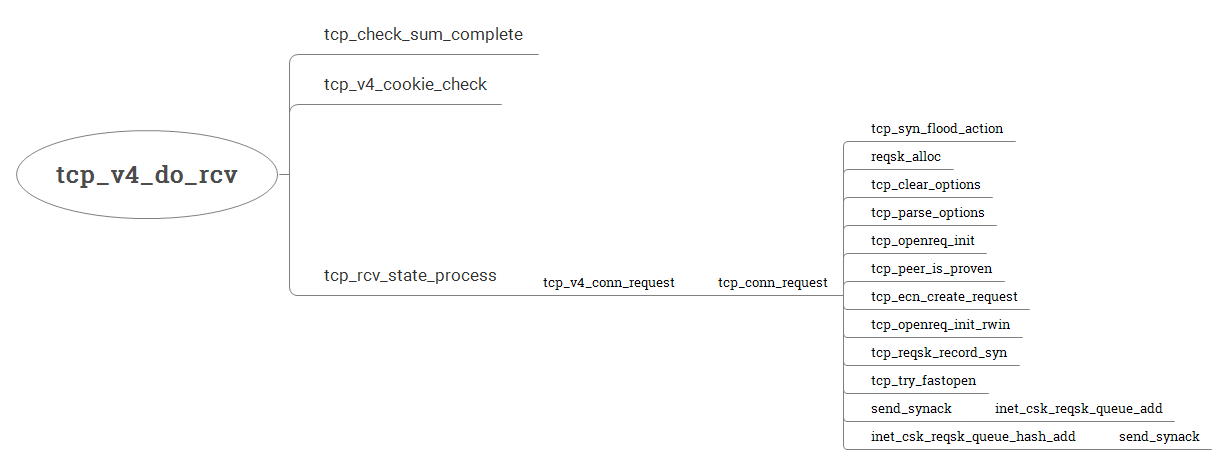
\includegraphics[width=\textwidth]  {images/The First Shake Hand of Server.png}
                \end{figure}       
            \subsubsection{\mintinline{C}{tcp_v4_do_rcv}}
                在进行第一次握手的时候,TCP必然处于LISTEN状态。传输控制块接收处理的段都由\mintinline{C}{tcp_v4_do_rcv}来处理。该函数位于/net/ipv4/tcp\_ipv4.c中。该函数会根据不同的TCP状态进行不同的处理,这里我们只是讨论服务器第一次握手的函数处理过程。
\begin{minted}[linenos]{C}
/* The socket must have it's spinlock held when we get
 * here, unless it is a TCP_LISTEN socket.
 *
 * We have a potential double-lock case here, so even when
 * doing backlog processing we use the BH locking scheme.
 * This is because we cannot sleep with the original spinlock
 * held.
 */
int tcp_v4_do_rcv(struct sock *sk, struct sk_buff *skb)
{
    struct sock *rsk;

    /*省略无关代码*/

    if (tcp_checksum_complete(skb))
        goto csum_err;

    if (sk->sk_state == TCP_LISTEN) {
        struct sock *nsk = tcp_v4_cookie_check(sk, skb);

        if (!nsk)
            goto discard;
        if (nsk != sk) {
            sock_rps_save_rxhash(nsk, skb);
            sk_mark_napi_id(nsk, skb);
            if (tcp_child_process(sk, nsk, skb)) {
                rsk = nsk;
                goto reset;
            }
            return 0;
        }
    } else
        sock_rps_save_rxhash(sk, skb);

    if (tcp_rcv_state_process(sk, skb)) {
        rsk = sk;
        goto reset;
    }
    return 0;

reset:
    tcp_v4_send_reset(rsk, skb);
discard:
    kfree_skb(skb);
    /* Be careful here. If this function gets more complicated and
     * gcc suffers from register pressure on the x86, sk (in \%ebx)
     * might be destroyed here. This current version compiles correctly,
     * but you have been warned.
     */
    return 0;

csum_err:
    TCP_INC_STATS_BH(sock_net(sk), TCP_MIB_CSUMERRORS);
    TCP_INC_STATS_BH(sock_net(sk), TCP_MIB_INERRS);
    goto discard;
}
\end{minted}

                首先,程序先基于伪首部累加和进行全包的校验和,判断包是否传输正确。

                其次,程序会进行相应的cookie检查。

                最后,程序会继续调用\mintinline{C}{tcp_rcv_state_process}函数处理接收到的SYN段。
            
            \subsubsection{\mintinline{C}{tcp_v4_cookie_check}}
                该函数如下:
\begin{minted}[linenos]{C}
static struct sock *tcp_v4_cookie_check(struct sock *sk, struct sk_buff *skb)
{
#ifdef CONFIG_SYN_COOKIES
    const struct tcphdr *th = tcp_hdr(skb);

    if (!th->syn)
        sk = cookie_v4_check(sk, skb);
#endif
    return sk;
}
\end{minted}

                一般情况下,当前linux内核都会定义\mintinline{C}{CONFIG_SYN_COOKIES}宏的,显然对于第一次握手的时候,接收到的确实是syn包,故而直接返回了sk。
            \subsubsection{\mintinline{C}{tcp_rcv_state_process}}
                该函数位于\mintinline{C}{/net/ipv4/tcp_input.c}中。与第一次握手相关的代码如下:

\begin{minted}[linenos]{C}
/*
 *  This function implements the receiving procedure of RFC 793 for
 *  all states except ESTABLISHED and TIME_WAIT.
 *  It's called from both tcp_v4_rcv and tcp_v6_rcv and should be
 *  address independent.
 */

int tcp_rcv_state_process(struct sock *sk, struct sk_buff *skb)
{
    struct tcp_sock *tp = tcp_sk(sk);
    struct inet_connection_sock *icsk = inet_csk(sk);
    const struct tcphdr *th = tcp_hdr(skb);
    struct request_sock *req;
    int queued = 0;
    bool acceptable;

    tp->rx_opt.saw_tstamp = 0;  /*saw_tstamp 表示在最新的包上是否看到的时间戳选项*/

    switch (sk->sk_state) {
    /*省略无关代码*/

		case TCP_LISTEN:
		    if (th->ack)
		        return 1;

		    if (th->rst)
		        goto discard;

		    if (th->syn) {
		        if (th->fin)
		            goto discard;
		        if (icsk->icsk_af_ops->conn_request(sk, skb) < 0)
		            return 1;

		        /* Now we have several options: In theory there is
		         * nothing else in the frame. KA9Q has an option to
		         * send data with the syn, BSD accepts data with the
		         * syn up to the [to be] advertised window and
		         * Solaris 2.1 gives you a protocol error. For now
		         * we just ignore it, that fits the spec precisely
		         * and avoids incompatibilities. It would be nice in
		         * future to drop through and process the data.
		         *
		         * Now that TTCP is starting to be used we ought to
		         * queue this data.
		         * But, this leaves one open to an easy denial of
		         * service attack, and SYN cookies can't defend
		         * against this problem. So, we drop the data
		         * in the interest of security over speed unless
		         * it's still in use.
		         */
		        kfree_skb(skb);
		        return 0;
		    }
		    goto discard;

		    /*省略无关代码*/
discard:
        __kfree_skb(skb);
    }
    return 0;
}
\end{minted}

                显然,所接收到的包的ack、rst、fin字段都不为1,故而这时开始进行连接检查,判断是否可以允许连接。经过不断查找,我们发现\mintinline{C}{icsk->icsk_af_ops->conn_request}最终会掉用\mintinline{C}{tcp_v4_conn_request}进行处理。如果syn段合法,内核就会为该连接请求创建连接请求块,并且保存相应的信息。否则,就会返回1,原函数会发送reset给客户端表明连接请求失败。

                当然,如果收到的包的ack字段为1,那么由于此时链接还未建立,故该包无效,返回1,并且调用该函数的函数会发送reset包给对方。如果收到的是rst字段或者既有fin又有syn的字段,那就直接销毁,并且释放内存。

            \subsubsection{\mintinline{C}{tcp_v4_conn_request && tcp_conn_request}}

                该函数位于\mintinline{C}{/net/ipv4/tcp_ipv4/tcp_ipv4.c}中,函数如下:
\begin{minted}[linenos]{C}
int tcp_v4_conn_request(struct sock *sk, struct sk_buff *skb)
{
    /* Never answer to SYNs send to broadcast or multicast */
    if (skb_rtable(skb)->rt_flags & (RTCF_BROADCAST | RTCF_MULTICAST))
        goto drop;

    return tcp_conn_request(&tcp_request_sock_ops,
                &tcp_request_sock_ipv4_ops, sk, skb);

drop:
    NET_INC_STATS_BH(sock_net(sk), LINUX_MIB_LISTENDROPS);
    return 0;
}
\end{minted}
                
        如果一个SYN段是要被发送到广播地址和组播地址,则直接drop掉,然后返回0。否则的话,就继续调用\mintinline{C}{tcp_conn_request}进行连接处理。

\begin{minted}[linenos]{C}
int tcp_conn_request(struct request_sock_ops *rsk_ops,
             const struct tcp_request_sock_ops *af_ops,
             struct sock *sk, struct sk_buff *skb)
{
    struct tcp_fastopen_cookie foc = { .len = -1 };		//初始化len字段
    __u32 isn = TCP_SKB_CB(skb)->tcp_tw_isn;			//tw???    isn: initial sequence num 初始化序列号 
    struct tcp_options_received tmp_opt;
    struct tcp_sock *tp = tcp_sk(sk);
    struct sock *fastopen_sk = NULL;
    struct dst_entry *dst = NULL;
    struct request_sock *req;
    bool want_cookie = false;							//???
    struct flowi fl;									//路由查找相关的数据结构

    /* TW buckets are converted to open requests without
     * limitations, they conserve resources and peer is
     * evidently real one.
     */
    if ((sysctl_tcp_syncookies == 2 ||
         inet_csk_reqsk_queue_is_full(sk)) && !isn) {
        want_cookie = tcp_syn_flood_action(sk, skb, rsk_ops->slab_name);
        if (!want_cookie)
            goto drop;
    }
\end{minted}
                首先,前面???如果SYN请求队列已满并且isn为0,然后通过函数\textbf{tcp\_syn\_flood\_action}判断是否需要发送syncookie。如果没有启用syncookie的话,就会返回false,此时不能接收新的SYN请求,会将所收到的包丢掉。
\begin{minted}[linenos]{C}
    /* Accept backlog is full. If we have already queued enough
     * of warm entries in syn queue, drop request. It is better than
     * clogging syn queue with openreqs with exponentially increasing
     * timeout.
     */
    if (sk_acceptq_is_full(sk) && inet_csk_reqsk_queue_young(sk) > 1) {
        NET_INC_STATS_BH(sock_net(sk), LINUX_MIB_LISTENOVERFLOWS);
        goto drop;
    }
\end{minted}

        \textbf{warm entries}               
        
        如果连接队列长度已经达到上限且SYN请求队列中至少有一个握手过程中没有重传过段,则丢弃当前请求。

\begin{minted}[linenos]{C}
    req = inet_reqsk_alloc(rsk_ops, sk, !want_cookie);
    if (!req)
        goto drop;
\end{minted}
            
        这时调用reqsk\_alloc()分配一个连接请求块,用于保存连接请求信息,同时初始化在连接过程中用来发送ACK/RST段的操作集合,以便在建立连接过程中能方便地调用这些接口。

\begin{minted}[linenos]{C}
    tcp_rsk(req)->af_specific = af_ops;
\end{minted}

        这一步进行的是为了保护BGP会话。???
        
\begin{minted}[linenos]{C}
    tcp_rsk(req)->af_specific = af_ops;

    tcp_clear_options(&tmp_opt);
    tmp_opt.mss_clamp = af_ops->mss_clamp;
    tmp_opt.user_mss  = tp->rx_opt.user_mss;
    tcp_parse_options(skb, &tmp_opt, 0, want_cookie ? NULL : &foc);
\end{minted}

        之后,清除TCP选项后初始化mss\_vlamp和user\_mss.然后调用tcp\_parse\_options解析SYN段中的TCP选项,查看是否有相关的选项。
\begin{minted}[linenos]{C}
    if (want_cookie && !tmp_opt.saw_tstamp)
        tcp_clear_options(&tmp_opt);
\end{minted}

        如果启动了syncookies,并且TCP段中没有存在时间戳(why,the reason?),则清除已经解析的TCP选项。

\begin{minted}[linenos]{C}
    tmp_opt.tstamp_ok = tmp_opt.saw_tstamp;
    tcp_openreq_init(req, &tmp_opt, skb, sk);
\end{minted}

        这时,根据收到的SYN段中的选项和序号来初始化连接请求块信息。

\begin{minted}[linenos]{C}
    /* Note: tcp_v6_init_req() might override ir_iif for link locals */
    inet_rsk(req)->ir_iif = sk->sk_bound_dev_if;

    af_ops->init_req(req, sk, skb);

    if (security_inet_conn_request(sk, skb, req))
        goto drop_and_free;
\end{minted}

        这一部分于IPV6以及安全检测有关,这里不进行详细讲解。安全检测失败的话,就会丢弃SYN段。

\begin{minted}[linenos]{C}
    if (!want_cookie && !isn) {
        /* VJ's idea. We save last timestamp seen
         * from the destination in peer table, when entering
         * state TIME-WAIT, and check against it before
         * accepting new connection request.
         *
         * If "isn" is not zero, this request hit alive
         * timewait bucket, so that all the necessary checks
         * are made in the function processing timewait state.
         */
        if (tcp_death_row.sysctl_tw_recycle) {
            bool strict;

            dst = af_ops->route_req(sk, &fl, req, &strict);

            if (dst && strict &&
                !tcp_peer_is_proven(req, dst, true,
                        tmp_opt.saw_tstamp)) {
                NET_INC_STATS_BH(sock_net(sk), LINUX_MIB_PAWSPASSIVEREJECTED);
                goto drop_and_release;
            }
        }
        /* Kill the following clause, if you dislike this way. */
        else if (!sysctl_tcp_syncookies &&
             (sysctl_max_syn_backlog - inet_csk_reqsk_queue_len(sk) <
              (sysctl_max_syn_backlog >> 2)) &&
             !tcp_peer_is_proven(req, dst, false,
                         tmp_opt.saw_tstamp)) {
            /* Without syncookies last quarter of
             * backlog is filled with destinations,
             * proven to be alive.
             * It means that we continue to communicate
             * to destinations, already remembered
             * to the moment of synflood.
             */
            pr_drop_req(req, ntohs(tcp_hdr(skb)->source),
                    rsk_ops->family);
            goto drop_and_release;
        }

        isn = af_ops->init_seq(skb);
    }
\end{minted}

        如果没有开启syncookie并且isn为0的话,在距中的第一个if从对段信息块中获取时间戳,在新的连接请求之前检测\textbf{PAWS}。后边的表明在没有启动syncookies的情况下受到synflood攻击,丢弃收到的段。之后由源地址,源端口,目的地址以及目的端口计算出服务端初始序列号。

\begin{minted}[linenos]{C}
    if (!dst) {
        dst = af_ops->route_req(sk, &fl, req, NULL);
        if (!dst)
            goto drop_and_free;
    }

    tcp_ecn_create_request(req, skb, sk, dst);

    if (want_cookie) {
        isn = cookie_init_sequence(af_ops, sk, skb, &req->mss);
        req->cookie_ts = tmp_opt.tstamp_ok;
        if (!tmp_opt.tstamp_ok)
            inet_rsk(req)->ecn_ok = 0;
    }

    tcp_rsk(req)->snt_isn = isn;
    tcp_rsk(req)->txhash = net_tx_rndhash();
    tcp_openreq_init_rwin(req, sk, dst);
    if (!want_cookie) {
        tcp_reqsk_record_syn(sk, req, skb);
        fastopen_sk = tcp_try_fastopen(sk, skb, req, &foc, dst);
    }
    if (fastopen_sk) {
        af_ops->send_synack(fastopen_sk, dst, &fl, req,
                    &foc, false);
        /* Add the child socket directly into the accept queue */
        inet_csk_reqsk_queue_add(sk, req, fastopen_sk);
        sk->sk_data_ready(sk);
        bh_unlock_sock(fastopen_sk);
        sock_put(fastopen_sk);
    } else {
        tcp_rsk(req)->tfo_listener = false;
        if (!want_cookie)
            inet_csk_reqsk_queue_hash_add(sk, req, TCP_TIMEOUT_INIT);
        af_ops->send_synack(sk, dst, &fl, req,
                    &foc, !want_cookie);
        if (want_cookie)
            goto drop_and_free;
    }
    reqsk_put(req);
    return 0;

drop_and_release:
    dst_release(dst);
drop_and_free:
    reqsk_free(req);
drop:
    NET_INC_STATS_BH(sock_net(sk), LINUX_MIB_LISTENDROPS);
    return 0;
\end{minted}

                暂时不懂,,,,等等在分析。。。。。。。

            \subsubsection{inet\_csk\_reqsk\_queue\_add}

\begin{minted}[linenos]{C}
struct sock *inet_csk_reqsk_queue_add(struct sock *sk,
                      struct request_sock *req,
                      struct sock *child)
{
    struct request_sock_queue *queue = &inet_csk(sk)->icsk_accept_queue;

    spin_lock(&queue->rskq_lock);
    if (unlikely(sk->sk_state != TCP_LISTEN)) {
        inet_child_forget(sk, req, child);
        child = NULL;
    } else {
        req->sk = child;
        req->dl_next = NULL;
        if (queue->rskq_accept_head == NULL)
            queue->rskq_accept_head = req;
        else
            queue->rskq_accept_tail->dl_next = req;
        queue->rskq_accept_tail = req;
        sk_acceptq_added(sk);
    }
    spin_unlock(&queue->rskq_lock);
    return child;
}
\end{minted}

                这一个函数所进行的操作就是直接将请求挂在接收队列中。

            \subsubsection{inet\_csk\_reqsk\_queue\_hash\_add}

\begin{minted}[linenos]{C}
void inet_csk_reqsk_queue_hash_add(struct sock *sk, struct request_sock *req,
                   unsigned long timeout)
{
    reqsk_queue_hash_req(req, timeout);
    inet_csk_reqsk_queue_added(sk);
}
\end{minted}

                首先将连接请求块保存到父传输请求块的散列表中,并设置定时器超时时间。之后更新已存在的连接请求块数,并启动连接建立定时器。
%----------------------------------------------------------------------------------------
%                   Server:     Send    SYN+ACK
%----------------------------------------------------------------------------------------

        \subsection{第二次握手:发送SYN+ACK段}
            在第一次握手的最后调用了af\_ops->send\_synack函数,而该函数最终会调用tcp\_v4\_send\_synack函数进行发送,故而这里我们这里就从这个函数进行分析。
            \subsubsection{第二次函数调用关系}            
                第二次握手的调用函数关系图如下:
                \begin{figure}[htb]        
                   \center{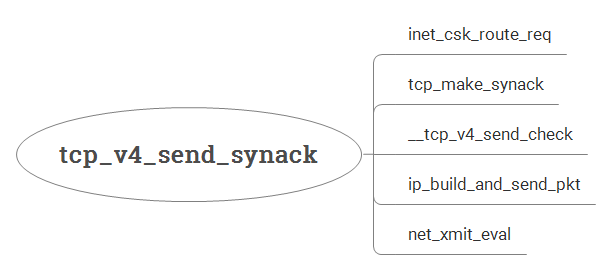
\includegraphics[width=\textwidth]  {images/The Second Shake Hand of Server.png}}
                \end{figure}   
            \subsubsection{tcp\_v4\_send\_synack}
\begin{minted}[linenos]{C}
/*
 *  Send a SYN-ACK after having received a SYN.
 *  This still operates on a request_sock only, not on a big
 *  socket.
 */
static int tcp_v4_send_synack(const struct sock *sk, struct dst_entry *dst,
                  struct flowi *fl,
                  struct request_sock *req,
                  struct tcp_fastopen_cookie *foc,
                  bool attach_req)
{
    const struct inet_request_sock *ireq = inet_rsk(req);
    struct flowi4 fl4;
    int err = -1;
    struct sk_buff *skb;

    /* First, grab a route. */
    if (!dst && (dst = inet_csk_route_req(sk, &fl4, req)) == NULL)
        return -1;

    skb = tcp_make_synack(sk, dst, req, foc, attach_req);

    if (skb) {
        __tcp_v4_send_check(skb, ireq->ir_loc_addr, ireq->ir_rmt_addr);

        err = ip_build_and_send_pkt(skb, sk, ireq->ir_loc_addr,
                        ireq->ir_rmt_addr,
                        ireq->opt);
        err = net_xmit_eval(err);
    }

    return err;
}
\end{minted}                
                首先,如果传进来的dst为空或者根据连接请求块中的信息查询路由表,如果没有查到,那么就直接推出。

                否则就跟据当前的传输控制块,路由信息,请求等信息构建syn+ack段。

                如果构建成功的话,就生成TCP校验码,然后调用ip\_build\_and\_send\_pkt生成IP数据报并且发送出去。

                net\_xmit\_eval是什么,待考虑。
            \subsubsection{tcp\_make\_synack}
                该函数用来构造一个SYN+ACK段,并初始化TCP首部及SKB中的各字段项,填入相应的选项,如MSS,SACK,窗口扩大银子,时间戳等。函数如下:
\begin{minted}[linenos]{C}
/**
 * tcp_make_synack - Prepare a SYN-ACK.
 * sk: listener socket
 * dst: dst entry attached to the SYNACK
 * req: request_sock pointer
 *
 * Allocate one skb and build a SYNACK packet.
 * @dst is consumed : Caller should not use it again.
 */
struct sk_buff *tcp_make_synack(const struct sock *sk, struct dst_entry *dst,
                struct request_sock *req,
                struct tcp_fastopen_cookie *foc,
                bool attach_req)
{
    struct inet_request_sock *ireq = inet_rsk(req);
    const struct tcp_sock *tp = tcp_sk(sk);
    struct tcp_md5sig_key *md5 = NULL;
    struct tcp_out_options opts;
    struct sk_buff *skb;
    int tcp_header_size;
    struct tcphdr *th;
    u16 user_mss;
    int mss;

    skb = alloc_skb(MAX_TCP_HEADER, GFP_ATOMIC);
    if (unlikely(!skb)) {
        dst_release(dst);
        return NULL;
    }
\end{minted}

                首先为将要发送的数据申请发送缓存,\textbf{unlikely函数待分析???},如果没有申请到,那就会返回NULL。

\begin{minted}[linenos]{C}
    /* Reserve space for headers. */
    skb_reserve(skb, MAX_TCP_HEADER);
\end{minted}

                为MAC层,IP层,TCP层首部预留必要的空间。

\begin{minted}[linenos]{C}
    if (attach_req) {
        skb_set_owner_w(skb, req_to_sk(req));
    } else {
        /* sk is a const pointer, because we want to express multiple
         * cpu might call us concurrently.
         * sk->sk_wmem_alloc in an atomic, we can promote to rw.
         */
        skb_set_owner_w(skb, (struct sock *)sk);
    }
    skb_dst_set(skb, dst);
\end{minted}

                根据\mintinline{C}{attach_req}来判断该执行如何执行相关操作\textbf{to do in the future}。然后设置发送缓存的目的路由\textbf{a little confused, why need this}。

\begin{minted}[linenos]{C}
    mss = dst_metric_advmss(dst);
    user_mss = READ_ONCE(tp->rx_opt.user_mss);
    if (user_mss && user_mss < mss)
        mss = user_mss;
\end{minted}

                根据每一个路由器上的mss以及自身的mss来得到最大的mss。
\begin{minted}[linenos]{C}
    memset(&opts, 0, sizeof(opts));
#ifdef CONFIG_SYN_COOKIES
    if (unlikely(req->cookie_ts))
        skb->skb_mstamp.stamp_jiffies = cookie_init_timestamp(req);
    else
#endif
    skb_mstamp_get(&skb->skb_mstamp);
\end{minted}

                清除选项,并且设置相关时间戳\textbf{to add in future}。


\begin{minted}[linenos]{C}
#ifdef CONFIG_TCP_MD5SIG
    rcu_read_lock();
    md5 = tcp_rsk(req)->af_specific->req_md5_lookup(sk, req_to_sk(req));
#endif
\end{minted}

                查看是否有MD5选项,有的话构造出相应的md5.

\begin{minted}[linenos]{C}
    skb_set_hash(skb, tcp_rsk(req)->txhash, PKT_HASH_TYPE_L4);
    tcp_header_size = tcp_synack_options(req, mss, skb, &opts, md5, foc) +
              sizeof(*th);

    skb_push(skb, tcp_header_size);
    skb_reset_transport_header(skb);
\end{minted}

                得到tcp的头部大小,然后进行大小设置,并且重置传输层的头部。

\begin{minted}[linenos]{C}
    th = tcp_hdr(skb);
    memset(th, 0, sizeof(struct tcphdr));
    th->syn = 1;
    th->ack = 1;
    tcp_ecn_make_synack(req, th);
    th->source = htons(ireq->ir_num);
    th->dest = ireq->ir_rmt_port;
\end{minted}

                清空tcp头部,并设置tcp头部的各个字段。

\begin{minted}[linenos]{C}
    /* Setting of flags are superfluous here for callers (and ECE is
     * not even correctly set)
     */
    tcp_init_nondata_skb(skb, tcp_rsk(req)->snt_isn,
                 TCPHDR_SYN | TCPHDR_ACK);

    th->seq = htonl(TCP_SKB_CB(skb)->seq);
    /* XXX data is queued and acked as is. No buffer/window check */
    th->ack_seq = htonl(tcp_rsk(req)->rcv_nxt);

    /* RFC1323: The window in SYN & SYN/ACK segments is never scaled. */
    th->window = htons(min(req->rsk_rcv_wnd, 65535U));
    tcp_options_write((__be32 *)(th + 1), NULL, &opts);
    th->doff = (tcp_header_size >> 2);
    TCP_INC_STATS_BH(sock_net(sk), TCP_MIB_OUTSEGS);
\end{minted}

                首先初始化不含数据的tcp报文,然后设置相关的序列号,确认序列号,窗口大小,选项字段,以及TCP数据偏移,之所以除以,是因为稿子短的单位时32位字,即以四个字节长的字为计算单位。
                
\begin{minted}[linenos]{C}
#ifdef CONFIG_TCP_MD5SIG
    /* Okay, we have all we need - do the md5 hash if needed */
    if (md5)
        tcp_rsk(req)->af_specific->calc_md5_hash(opts.hash_location,
                           md5, req_to_sk(req), skb);
    rcu_read_unlock();
#endif

    /* Do not fool tcpdump (if any), clean our debris */
    skb->tstamp.tv64 = 0;
    return skb;
}
\end{minted}

                最后判断是否需要md5哈希值,如果需要的话,就进行添加。\textbf{what does it mean in the middle?},然后返回生成包含SYN+ACK段的skb。     

        \subsection{第三次握手:接收ACK段}

                在服务器第二次我受的最后启动了建立连接定时器,等待客户端最后一次握手的ACK段。           
                \subsubsection{第三次握手函数调用关系图}
                \subsubsection{tcp\_v4\_do\_rcv}
\begin{minted}[linenos]{C}
/* The socket must have it's spinlock held when we get
 * here, unless it is a TCP_LISTEN socket.
 *
 * We have a potential double-lock case here, so even when
 * doing backlog processing we use the BH locking scheme.
 * This is because we cannot sleep with the original spinlock
 * held.
 */
int tcp_v4_do_rcv(struct sock *sk, struct sk_buff *skb)
{
    struct sock *rsk;

    /**省略无关代码**/

    if (tcp_checksum_complete(skb))
        goto csum_err;

    if (sk->sk_state == TCP_LISTEN) {
        struct sock *nsk = tcp_v4_cookie_check(sk, skb);

        if (!nsk)
            goto discard;
        if (nsk != sk) {
            sock_rps_save_rxhash(nsk, skb);
            sk_mark_napi_id(nsk, skb);
            if (tcp_child_process(sk, nsk, skb)) {
                rsk = nsk;
                goto reset;
            }
            return 0;
        }
    } else
        sock_rps_save_rxhash(sk, skb);
    /**省略无关代码**/
reset:
    tcp_v4_send_reset(rsk, skb);
discard:
    kfree_skb(skb);
    /* Be careful here. If this function gets more complicated and
     * gcc suffers from register pressure on the x86, sk (in %ebx)
     * might be destroyed here. This current version compiles correctly,
     * but you have been warned.
     */
    return 0;

csum_err:
    TCP_INC_STATS_BH(sock_net(sk), TCP_MIB_CSUMERRORS);
    TCP_INC_STATS_BH(sock_net(sk), TCP_MIB_INERRS);
    goto discard;
}
\end{minted}
                    在服务器最后一次握手的时候,其实传输控制块仍然处于LISTEN状态,但是这时候cookie检查得到的传输控制块已经不是侦听传输控制快了,故而会执行\mintinline{C}{tcp_child_process}来初始化子传输控制块。如果初始化失败的话(返回值非零),就会给客户端发送RST段进行复位。

                \subsubsection{tcp\_v4\_cookie\_check}

\begin{minted}[linenos]{C}
static struct sock *tcp_v4_cookie_check(struct sock *sk, struct sk_buff *skb)
{
#ifdef CONFIG_SYN_COOKIES
    const struct tcphdr *th = tcp_hdr(skb);

    if (!th->syn)
        sk = cookie_v4_check(sk, skb);
#endif
    return sk;
}
\end{minted}

                    在现在的Linux内核中一般都会定义\mintinline{C}{CONFIG_SYN_COOKIES}宏,此时在第三次握手阶段,并不是 syn包,内核就会执行\mintinline{C}{cookie_v4_check}。在这个函数中,服务器会将客户端的ACK序列号减去1,得到cookie比较值,然后将客户端的IP地址,客户端端口,服务器IP地址和服务器端口,接收到的TCP序列好以及其它一些安全数值等要素进行hash运算后,与该cookie比较值比较,如果相等,则直接完成三次握手,此时不必查看该连接是否属于请求连接队列。

                \subsubsection{tcp\_child\_process}

                    子传输控制块开始处理TCP段。
\begin{minted}[linenos]{C}
/*
 * Queue segment on the new socket if the new socket is active,
 * otherwise we just shortcircuit this and continue with
 * the new socket.
 *
 * For the vast majority of cases child->sk_state will be TCP_SYN_RECV
 * when entering. But other states are possible due to a race condition
 * where after __inet_lookup_established() fails but before the listener
 * locked is obtained, other packets cause the same connection to
 * be created.
 */

int tcp_child_process(struct sock *parent, struct sock *child,
              struct sk_buff *skb)
{
    int ret = 0;
    int state = child->sk_state;

    tcp_sk(child)->segs_in += max_t(u16, 1, skb_shinfo(skb)->gso_segs);
    if (!sock_owned_by_user(child)) {
        ret = tcp_rcv_state_process(child, skb);
        /* Wakeup parent, send SIGIO */
        if (state == TCP_SYN_RECV && child->sk_state != state)
            parent->sk_data_ready(parent);
    } else {
        /* Alas, it is possible again, because we do lookup
         * in main socket hash table and lock on listening
         * socket does not protect us more.
         */
        __sk_add_backlog(child, skb);
    }

    bh_unlock_sock(child);
    sock_put(child);
    return ret;
}
\end{minted}

                该函数位于\mintinline{C}{tcp_minisocks.c}中。

                首先,如果此时刚刚创建的新的子传输控制块没有被用户进程占用,则根据作为第三次握手的ACK段,调用\mintinline{C}{tcp_rcv_state_process}继续对子传输控制块做初始化。否则的话,只能将其加入后备队列中,等空闲时再进行处理。虽然这种情况出现的概率小,但是也是有可能发生的。

                \subsubsection{tcp\_rcv\_state\_process}

                    该函数用来处理ESTABLISHED和\mintinline{C}{TIME_WAIT}状态以外的TCP段,这里处理\mintinline{C}{SYN_RECV}状态。
\begin{minted}[linenos]{C}
    acceptable = tcp_ack(sk, skb, FLAG_SLOWPATH |
                      FLAG_UPDATE_TS_RECENT) > 0;
\end{minted}

                    首先对收到的ACK段进行处理判断是否正确接收,如果正确接收就会发送返回非零值。

\begin{minted}[linenos]{C}
    switch (sk->sk_state) {
        case TCP_SYN_RECV:
            if (!acceptable)
                return 1;

            if (!tp->srtt_us)
                tcp_synack_rtt_meas(sk, req);

            /* Once we leave TCP_SYN_RECV, we no longer need req
             * so release it.
             */
            if (req) {
                tp->total_retrans = req->num_retrans;
                reqsk_fastopen_remove(sk, req, false);
            } else {
                /* Make sure socket is routed, for correct metrics. */
                icsk->icsk_af_ops->rebuild_header(sk);
                tcp_init_congestion_control(sk);

                tcp_mtup_init(sk);
                tp->copied_seq = tp->rcv_nxt;
                tcp_init_buffer_space(sk);
            }
            smp_mb();
            tcp_set_state(sk, TCP_ESTABLISHED);
            sk->sk_state_change(sk);
\end{minted}

                    进行一系列的初始化,开启相应拥塞控制等,并且将TCP的状态置为ESTABLISHED。

\begin{minted}[linenos]{C}

            /* Note, that this wakeup is only for marginal crossed SYN case.
             * Passively open sockets are not waked up, because
             * sk->sk_sleep == NULL and sk->sk_socket == NULL.
             */
            if (sk->sk_socket)
                sk_wake_async(sk, SOCK_WAKE_IO, POLL_OUT);
\end{minted}

                    发信号给那些将通过该套接口发送数据的进程,通知它们套接口目前已经可以发送数据了。

\begin{minted}[linenos]{C}
            tp->snd_una = TCP_SKB_CB(skb)->ack_seq;
            tp->snd_wnd = ntohs(th->window) << tp->rx_opt.snd_wscale;
            tcp_init_wl(tp, TCP_SKB_CB(skb)->seq);

            if (tp->rx_opt.tstamp_ok)
                tp->advmss -= TCPOLEN_TSTAMP_ALIGNED;
\end{minted}

                    初始化传输控制块的各个字段,对时间戳进行处理。

\begin{minted}[linenos]{C}
            if (req) {
                /* Re-arm the timer because data may have been sent out.
                 * This is similar to the regular data transmission case
                 * when new data has just been ack'ed.
                 *
                 * (TFO) - we could try to be more aggressive and
                 * retransmitting any data sooner based on when they
                 * are sent out.
                 */
                tcp_rearm_rto(sk);
            } else
                tcp_init_metrics(sk);
\end{minted}

                    为该套接口初始化路由。

\begin{minted}[linenos]{C}
            tcp_update_pacing_rate(sk);

            /* Prevent spurious tcp_cwnd_restart() on first data packet */
            tp->lsndtime = tcp_time_stamp;

            tcp_initialize_rcv_mss(sk);
            tcp_fast_path_on(tp);
            break;
\end{minted}

                更新最近一次的发送数据报的时间,初始化与路径MTU有关的成员,并计算有关TCP首部预测的标志。

\begin{minted}[linenos]{C}
    /* step 6: check the URG bit */
    tcp_urg(sk, skb, th);
\end{minted}

                检测带外数据标志位。

\begin{minted}[linenos]{C}
    /* step 7: process the segment text */
    switch (sk->sk_state) {
        /**省略无关代码**/
        case TCP_ESTABLISHED:
            tcp_data_queue(sk, skb);
            queued = 1;
            break;
    }
\end{minted}

                对已接收到的TCP段排队,在建立连接阶段一般不会收到TCP段。

\begin{minted}[linenos]{C}
    /* tcp_data could move socket to TIME-WAIT */
    if (sk->sk_state != TCP_CLOSE) {
        tcp_data_snd_check(sk);
        tcp_ack_snd_check(sk);
    }

    if (!queued) {
discard:
        __kfree_skb(skb);
    }
    return 0;
\end{minted}

                显然此时状态不为CLOSE,故而就回去检测是否数据和ACK要发送。其次,根据queue标志来确定是否释放接收到的TCP段,如果接收到的TCP段已添加到接收队列中,则不释放。


\chapter{TCP连接释放}
\minitoc
\section{主动关闭}
\label{sec:tcp_active_close}

\subsection{第一次握手——发送FIN}
\label{subsec:tcp_shutdown}
通过shutdown系统调用,主动关闭TCP连接。该系统调用最终由\mintinline{c}{tcp_shutdown}实现。
代码如下:

\begin{minted}[linenos]{c}
/*
Location:

	net/ipv4/tcp.c

Function:

	Shutdown the sending side of a connection. Much like close except
	that we don't receive shut down or sock_set_flag(sk, SOCK_DEAD).

Parameter:

	sk:传输控制块
	how:???
*/
void tcp_shutdown(struct sock *sk, int how)
{
        /*      We need to grab some memory, and put together a FIN,
         *      and then put it into the queue to be sent.
         *              Tim MacKenzie(tym@dibbler.cs.monash.edu.au) 4 Dec '92.
         */
        if (!(how & SEND_SHUTDOWN))
                return;

        /* 如果此时已经发送一个FIN了,就跳过。 */
        if ((1 << sk->sk_state) &
            (TCPF_ESTABLISHED | TCPF_SYN_SENT |
             TCPF_SYN_RECV | TCPF_CLOSE_WAIT)) {
                /* Clear out any half completed packets.  FIN if needed. */
                if (tcp_close_state(sk))
                        tcp_send_fin(sk);
        }
}
\end{minted}
该函数会在需要发送FIN时,调用\mintinline{c}{tcp_close_state()}来设置TCP的状态。
该函数会根据当前的状态,按照\ref{subsubsec:tcp_state_diagram}中给出的状态图。
\begin{minted}[linenos]{c}
static const unsigned char new_state[16] = {
  /* 当前状态:             新的状态:        动作:      */
  [0 /* (Invalid) */]   = TCP_CLOSE,
  [TCP_ESTABLISHED]     = TCP_FIN_WAIT1 | TCP_ACTION_FIN,
  [TCP_SYN_SENT]        = TCP_CLOSE,
  [TCP_SYN_RECV]        = TCP_FIN_WAIT1 | TCP_ACTION_FIN,
  [TCP_FIN_WAIT1]       = TCP_FIN_WAIT1,
  [TCP_FIN_WAIT2]       = TCP_FIN_WAIT2,
  [TCP_TIME_WAIT]       = TCP_CLOSE,
  [TCP_CLOSE]           = TCP_CLOSE,
  [TCP_CLOSE_WAIT]      = TCP_LAST_ACK  | TCP_ACTION_FIN,
  [TCP_LAST_ACK]        = TCP_LAST_ACK,
  [TCP_LISTEN]          = TCP_CLOSE,
  [TCP_CLOSING]         = TCP_CLOSING,
  [TCP_NEW_SYN_RECV]    = TCP_CLOSE,    /* should not happen ! */
};

static int tcp_close_state(struct sock *sk)
{
        int next = (int)new_state[sk->sk_state];
        int ns = next & TCP_STATE_MASK;

        /* 根据状态图进行状态转移 */
        tcp_set_state(sk, ns);

        /* 如果需要执行发送FIN的动作,则返回真 */
        return next & TCP_ACTION_FIN;
}
\end{minted}
可以看出,只有当当前状态为TCP\_ESTABLISHED、TCP\_SYN\_RECV、TCP\_CLOSE\_WAIT时,
需要发送FIN包。这个也和TCP状态图一致。如果需要发送FIN包,则会调用
\mintinline{c}{tcp_send_fin}。

\begin{minted}[linenos]{c}
void tcp_send_fin(struct sock *sk)
{
        struct sk_buff *skb, *tskb = tcp_write_queue_tail(sk);
        struct tcp_sock *tp = tcp_sk(sk);

        /* 这里做了一些优化,如果发送队列的末尾还有段没有发出去,则利用该段发送FIN。 */
        if (tskb && (tcp_send_head(sk) || tcp_under_memory_pressure(sk))) {
          /* 如果当前正在发送的队列不为空,或者当前TCP处于内存压力下,则进行该优化 */
coalesce:
                TCP_SKB_CB(tskb)->tcp_flags |= TCPHDR_FIN;
                TCP_SKB_CB(tskb)->end_seq++;
                tp->write_seq++;
                if (!tcp_send_head(sk)) {
                        /* This means tskb was already sent.
                         * Pretend we included the FIN on previous transmit.
                         * We need to set tp->snd_nxt to the value it would have
                         * if FIN had been sent. This is because retransmit path
                         * does not change tp->snd_nxt.
                         */
                        tp->snd_nxt++;
                        return;
                }
        } else {
                /* 为封包分配空间 */
                skb = alloc_skb_fclone(MAX_TCP_HEADER, sk->sk_allocation);
                if (unlikely(!skb)) {
                        /* 如果分配不到空间,且队尾还有未发送的包,利用该包发出FIN。 */
                        if (tskb)
                                goto coalesce;
                        return;
                }
                skb_reserve(skb, MAX_TCP_HEADER);
                sk_forced_mem_schedule(sk, skb->truesize);
                /* FIN eats a sequence byte, write_seq advanced by tcp_queue_skb(). */
                /* 构造一个FIN包,并加入发送队列。 */
                tcp_init_nondata_skb(skb, tp->write_seq,
                                     TCPHDR_ACK | TCPHDR_FIN);
                tcp_queue_skb(sk, skb);
        }
        __tcp_push_pending_frames(sk, tcp_current_mss(sk), TCP_NAGLE_OFF);
}
\end{minted}
在函数的最后,将所有的剩余数据一口气发出去,完成发送FIN包的过程。至此,主动关闭过程的
第一次握手完成。

\subsection{第二次握手——接受ACK}
在发出FIN后,接收端会回复ACK确认收到了请求。从这里开始有两种情况,这里先考虑教科书式
的四次握手的情况。双方同时发出FIN的情况会在\ref{subsec:fin_at_same_time}中描述。
根据状态图,主动发出FIN包后,会进入\mintinline{text}{FIN_WAIT1}状态。根据这一信息,
可以从\mintinline{c}{tcp_rcv_state_process}中,找到相应的代码。
\begin{minted}[linenos]{c}
int tcp_rcv_state_process(struct sock *sk, struct sk_buff *skb)
{
        struct tcp_sock *tp = tcp_sk(sk);
        struct inet_connection_sock *icsk = inet_csk(sk);
        const struct tcphdr *th = tcp_hdr(skb);
        struct request_sock *req;
        int queued = 0;
        bool acceptable;

        tp->rx_opt.saw_tstamp = 0;
        switch (sk->sk_state) {
        case TCP_CLOSE:
                goto discard;

        case TCP_LISTEN:
                /* LISTEN状态处理代码,略去 */

        case TCP_SYN_SENT:
                /* SYN-SENT状态处理代码,略去 */
        }

        /* fastopen相关代码及各类合法性判断,略去 */

        switch (sk->sk_state) {
        case TCP_SYN_RECV:
                /* SYN-RECV状态处理代码,略去 */
        
        case TCP_FIN_WAIT1: {
                struct dst_entry *dst;
                int tmo;

                /* 如果当前的套接字为开启了Fast Open的套接字,且该ACK为
                 * 接收到的第一个ACK,那么这个ACK应该是在确认SYNACK包,
                 * 因此,停止SYNACK计时器。
                 */
                if (req) {
                        /* Return RST if ack_seq is invalid.
                         * Note that RFC793 only says to generate a
                         * DUPACK for it but for TCP Fast Open it seems
                         * better to treat this case like TCP_SYN_RECV
                         * above.
                         */
                        if (!acceptable)
                                return 1;
                        /* 移除fastopen请求 */
                        reqsk_fastopen_remove(sk, req, false);
                        tcp_rearm_rto(sk);
                }
                if (tp->snd_una != tp->write_seq)
                        break;

                /* 收到ACK后,转移到TCP_FIN_WAIT2状态,将发送端关闭。 */
                tcp_set_state(sk, TCP_FIN_WAIT2);
                sk->sk_shutdown |= SEND_SHUTDOWN;

                /* 确认路由缓存有效 */
                dst = __sk_dst_get(sk);
                if (dst)
                        dst_confirm(dst);

                /* 唤醒等待该套接字的进程 */
                if (!sock_flag(sk, SOCK_DEAD)) {
                        /* Wake up lingering close() */
                        sk->sk_state_change(sk);
                        break;
                }

                /* 如果所有发送的字节都被确认了,那么进入关闭状态。 */
                if (tp->linger2 < 0 ||
                    (TCP_SKB_CB(skb)->end_seq != TCP_SKB_CB(skb)->seq &&
                     after(TCP_SKB_CB(skb)->end_seq - th->fin, tp->rcv_nxt))) {
                        tcp_done(sk);
                        NET_INC_STATS_BH(sock_net(sk), LINUX_MIB_TCPABORTONDATA);
                        return 1;
                }
\end{minted}
转换到\mintinline{c}{TCP_FIN_WAIT2}以后,计算接受fin包的超时时间。
如果还能留出TIMEWAIT阶段的时间(TIMEWAIT阶段有最长时间限制),那么在此之前,
就激活保活计时器保持连接。如果时间已经不足了,就主动调用\mintinline{c}{tcp_time_wait}
进入TIMEWAIT状态。
\begin{minted}[linenos]{c}
                tmo = tcp_fin_time(sk);
                if (tmo > TCP_TIMEWAIT_LEN) {
                        inet_csk_reset_keepalive_timer(sk, tmo - TCP_TIMEWAIT_LEN);
                } else if (th->fin || sock_owned_by_user(sk)) {
                        /* Bad case. We could lose such FIN otherwise.
                         * It is not a big problem, but it looks confusing
                         * and not so rare event. We still can lose it now,
                         * if it spins in bh_lock_sock(), but it is really
                         * marginal case.
                         */
                        inet_csk_reset_keepalive_timer(sk, tmo);
                } else {
                        /* 进入TCP_FIN_WAIT2状态等待。 */
                        tcp_time_wait(sk, TCP_FIN_WAIT2, tmo);
                        goto discard;
                }
                break;

                /* 其余状态处理代码,略去 */
        }

        /* step 6: check the URG bit */
        tcp_urg(sk, skb, th);

        /* step 7: process the segment text */
        switch (sk->sk_state) {
          /* 其他状态处理代码,略去 */

        case TCP_FIN_WAIT1:
        case TCP_FIN_WAIT2:
                /* RFC 793 says to queue data in these states,
                 * RFC 1122 says we MUST send a reset.
                 * BSD 4.4 also does reset.
                 */
                if (sk->sk_shutdown & RCV_SHUTDOWN) {
                        if (TCP_SKB_CB(skb)->end_seq != TCP_SKB_CB(skb)->seq &&
                            after(TCP_SKB_CB(skb)->end_seq - th->fin, tp->rcv_nxt)) {
                                NET_INC_STATS_BH(sock_net(sk), LINUX_MIB_TCPABORTONDATA);
                                /* 如果接收端已经关闭了,那么发送RESET。 */
                                tcp_reset(sk);
                                return 1;
                        }
                }
                /* Fall through */

           /* 其他状态处理代码,略去 */
        }

        /* tcp_data could move socket to TIME-WAIT */
        if (sk->sk_state != TCP_CLOSE) {
                tcp_data_snd_check(sk);
                tcp_ack_snd_check(sk);
        }

        if (!queued) {
discard:
                __kfree_skb(skb);
        }
        return 0;
}
\end{minted}
执行完该段代码后,则进入了\mintinline{text}{FIN_WAIT2}状态。

由于进入到\mintinline{text}{FIN_WAIT2}状态后,不会再处理TCP段的数据。
因此,出于资源和方面的考虑,采用了一个较小的结构体\mintinline{c}{tcp_timewait_sock}来
取代正常的TCP传输控制块。\mintinline{text}{TIME_WAIT}也是可作同样处理。
该替换过程通过函数\mintinline{c}{tcp_time_wait}完成。
\begin{minted}[linenos]{c}
void tcp_time_wait(struct sock *sk, int state, int timeo)
{
        const struct inet_connection_sock *icsk = inet_csk(sk);
        const struct tcp_sock *tp = tcp_sk(sk);
        struct inet_timewait_sock *tw;
        bool recycle_ok = false;

        if (tcp_death_row.sysctl_tw_recycle && tp->rx_opt.ts_recent_stamp)
                recycle_ok = tcp_remember_stamp(sk);

        /* 分配空间 */
        tw = inet_twsk_alloc(sk, &tcp_death_row, state);

        if (tw) {
                struct tcp_timewait_sock *tcptw = tcp_twsk((struct sock *)tw);
                const int rto = (icsk->icsk_rto << 2) - (icsk->icsk_rto >> 1);
                struct inet_sock *inet = inet_sk(sk);

                /* 将值复制给对应的域 */
                tw->tw_transparent      = inet->transparent;
                tw->tw_rcv_wscale       = tp->rx_opt.rcv_wscale;
                tcptw->tw_rcv_nxt       = tp->rcv_nxt;
                tcptw->tw_snd_nxt       = tp->snd_nxt;
                tcptw->tw_rcv_wnd       = tcp_receive_window(tp);
                tcptw->tw_ts_recent     = tp->rx_opt.ts_recent;
                tcptw->tw_ts_recent_stamp = tp->rx_opt.ts_recent_stamp;
                tcptw->tw_ts_offset     = tp->tsoffset;
                tcptw->tw_last_oow_ack_time = 0;

                /* 部分对于ipv6和md5的处理,略过 */

                /* Get the TIME_WAIT timeout firing. */
                if (timeo < rto)
                        timeo = rto;

                if (recycle_ok) {
                        tw->tw_timeout = rto;
                } else {
                        tw->tw_timeout = TCP_TIMEWAIT_LEN;
                        if (state == TCP_TIME_WAIT)
                                timeo = TCP_TIMEWAIT_LEN;
                }

                /* 启动定时器 */
                inet_twsk_schedule(tw, timeo);
                /* 将timewait控制块插入到哈希表中,替代原有的传输控制块 */
                __inet_twsk_hashdance(tw, sk, &tcp_hashinfo);
                inet_twsk_put(tw);
        } else {
                /* 当内存不够时,直接关闭连接 */
                NET_INC_STATS_BH(sock_net(sk), LINUX_MIB_TCPTIMEWAITOVERFLOW);
        }

        /* 更新一些测量值并关闭原来的传输控制块 */
        tcp_update_metrics(sk);
        tcp_done(sk);
}
\end{minted}

\subsection{第三次握手——接受FIN}
\label{subsec:third_recv_fin}
此时,由于已经使用了timewait控制块取代了TCP控制块。因此,对应的处理代码不再位于
\mintinline{c}{tcp_rcv_state_process}中,而是换到了
\mintinline{c}{tcp_timewait_state_process}函数中。该函数的代码如下,可以看到
参数中已经变成了\mintinline{c}{inet_timewait_sock}。
\begin{minted}[linenos]{c}
enum tcp_tw_status
tcp_timewait_state_process(struct inet_timewait_sock *tw, struct sk_buff *skb,
                           const struct tcphdr *th)
{
        struct tcp_options_received tmp_opt;
        struct tcp_timewait_sock *tcptw = tcp_twsk((struct sock *)tw);
        bool paws_reject = false;

        tmp_opt.saw_tstamp = 0;
        if (th->doff > (sizeof(*th) >> 2) && tcptw->tw_ts_recent_stamp) {
                tcp_parse_options(skb, &tmp_opt, 0, NULL);

                if (tmp_opt.saw_tstamp) {
                        tmp_opt.rcv_tsecr       -= tcptw->tw_ts_offset;
                        tmp_opt.ts_recent       = tcptw->tw_ts_recent;
                        tmp_opt.ts_recent_stamp = tcptw->tw_ts_recent_stamp;
                        paws_reject = tcp_paws_reject(&tmp_opt, th->rst);
                }
        }
\end{minted}
检测收到的包是否含有时间戳选项,如果有,则进行PAWS相关的检测。之后,开始进行
\mintinline{text}{TCP_FIN_WAIT2}相关的处理。
\begin{minted}[linenos]{c}
        if (tw->tw_substate == TCP_FIN_WAIT2) {
                /* 重复tcp_rcv_state_process()所进行的所有检测 */

                /* 序号不在窗口内,发送ACK */
                if (paws_reject ||
                    !tcp_in_window(TCP_SKB_CB(skb)->seq, TCP_SKB_CB(skb)->end_seq,
                                   tcptw->tw_rcv_nxt,
                                   tcptw->tw_rcv_nxt + tcptw->tw_rcv_wnd))
                        return tcp_timewait_check_oow_rate_limit(
                                tw, skb, LINUX_MIB_TCPACKSKIPPEDFINWAIT2);

                /* 如果收到RST包,则销毁timewait控制块并返回TCP_TW_SUCCESS */
                if (th->rst)
                        goto kill;

                /* 如果收到SYN包,则销毁并发送RST */
                if (th->syn && !before(TCP_SKB_CB(skb)->seq, tcptw->tw_rcv_nxt))
                        goto kill_with_rst;

                /* 如果收到DACK,则释放该控制块 */
                if (!th->ack ||
                    !after(TCP_SKB_CB(skb)->end_seq, tcptw->tw_rcv_nxt) ||
                    TCP_SKB_CB(skb)->end_seq == TCP_SKB_CB(skb)->seq) {
                        inet_twsk_put(tw);
                        return TCP_TW_SUCCESS;
                }

                /* 之后只有两种情况,有新数据或收到FIN包 */
                if (!th->fin ||
                    TCP_SKB_CB(skb)->end_seq != tcptw->tw_rcv_nxt + 1) {
                        /* 如果收到了新的数据或者序号有问题,
                         * 则销毁控制块并发送RST。 
                         */
kill_with_rst:
                        inet_twsk_deschedule_put(tw);
                        return TCP_TW_RST;
                }

                /* 收到了FIN包,进入TIME_WAIT状态 */
                tw->tw_substate   = TCP_TIME_WAIT;
                tcptw->tw_rcv_nxt = TCP_SKB_CB(skb)->end_seq;
                /* 如果启用了时间戳选项,则设置相关属性 */
                if (tmp_opt.saw_tstamp) {
                        tcptw->tw_ts_recent_stamp = get_seconds();
                        tcptw->tw_ts_recent       = tmp_opt.rcv_tsval;
                }

                /* 启动TIME_WAIT定时器 */
                if (tcp_death_row.sysctl_tw_recycle &&
                    tcptw->tw_ts_recent_stamp &&
                    tcp_tw_remember_stamp(tw))
                        inet_twsk_reschedule(tw, tw->tw_timeout);
                else
                        inet_twsk_reschedule(tw, TCP_TIMEWAIT_LEN);
                return TCP_TW_ACK;
        }

        /* TIME_WAIT阶段处理代码 */

}
\end{minted}

\subsection{第四次握手——发送ACK}
在\mintinline{c}{tcp_v4_rcv}中,如果发现目前的连接处于\mintinline{text}{FIN_WAIT2}
或\mintinline{text}{TIME_WAIT}状态,则调用\mintinline{c}{tcp_timewait_state_process}
进行处理,根据其返回值,执行相关操作。

\begin{minted}[linenos]{c}
switch (tcp_timewait_state_process(inet_twsk(sk), skb, th)) {
        case TCP_TW_SYN: {
                struct sock *sk2 = inet_lookup_listener(dev_net(skb->dev),
                                                        &tcp_hashinfo,
                                                        iph->saddr, th->source,
                                                        iph->daddr, th->dest,
                                                        inet_iif(skb));
                if (sk2) {
                        inet_twsk_deschedule_put(inet_twsk(sk));
                        sk = sk2;
                        goto process;
                }
                /* Fall through to ACK */
        }
        case TCP_TW_ACK:
                /* 回复ACK包 */
                tcp_v4_timewait_ack(sk, skb);
                break;
        case TCP_TW_RST:
                goto no_tcp_socket;
        case TCP_TW_SUCCESS:;
}
\end{minted}
根据上面的分析,在正常情况下,\mintinline{c}{tcp_timewait_state_process}会返回
\mintinline{c}{TCP_TW_ACK},因此,会调用\mintinline{c}{tcp_v4_timewait_ack}。
该函数如下:
\begin{minted}[linenos]{c}
static void tcp_v4_timewait_ack(struct sock *sk, struct sk_buff *skb)
{
        struct inet_timewait_sock *tw = inet_twsk(sk);
        struct tcp_timewait_sock *tcptw = tcp_twsk(sk);

        /* 发送ACK包 */
        tcp_v4_send_ack(sock_net(sk), skb,
                        tcptw->tw_snd_nxt, tcptw->tw_rcv_nxt,
                        tcptw->tw_rcv_wnd >> tw->tw_rcv_wscale,
                        tcp_time_stamp + tcptw->tw_ts_offset,
                        tcptw->tw_ts_recent,
                        tw->tw_bound_dev_if,
                        tcp_twsk_md5_key(tcptw),
                        tw->tw_transparent ? IP_REPLY_ARG_NOSRCCHECK : 0,
                        tw->tw_tos
                        );

        /* 释放timewait控制块 */
        inet_twsk_put(tw);
}
\end{minted}
紧接着又将发送ACK包的任务交给\mintinline{c}{tcp_v4_send_ack}来执行。
\begin{minted}[linenos]{c}
/* 下面的代码负责在SYN_RECV和TIME_WAIT状态下发送ACK包。
 *
 * The code following below sending ACKs in SYN-RECV and TIME-WAIT states
 * outside socket context is ugly, certainly. What can I do? 
 */
static void tcp_v4_send_ack(struct net *net,
                            struct sk_buff *skb, u32 seq, u32 ack,
                            u32 win, u32 tsval, u32 tsecr, int oif,
                            struct tcp_md5sig_key *key,
                            int reply_flags, u8 tos)
{
        const struct tcphdr *th = tcp_hdr(skb);
        struct {
                struct tcphdr th;
                __be32 opt[(TCPOLEN_TSTAMP_ALIGNED >> 2)
#ifdef CONFIG_TCP_MD5SIG
                           + (TCPOLEN_MD5SIG_ALIGNED >> 2)
#endif
                        ];
        } rep;
        struct ip_reply_arg arg;

        memset(&rep.th, 0, sizeof(struct tcphdr));
        memset(&arg, 0, sizeof(arg));

        /* 构造参数和TCP头部 */
        arg.iov[0].iov_base = (unsigned char *)&rep;
        arg.iov[0].iov_len  = sizeof(rep.th);
        if (tsecr) {
                rep.opt[0] = htonl((TCPOPT_NOP << 24) | (TCPOPT_NOP << 16) |
                                   (TCPOPT_TIMESTAMP << 8) |
                                   TCPOLEN_TIMESTAMP);
                rep.opt[1] = htonl(tsval);
                rep.opt[2] = htonl(tsecr);
                arg.iov[0].iov_len += TCPOLEN_TSTAMP_ALIGNED;
        }

        /* 交换发送端和接收端 */
        rep.th.dest    = th->source;
        rep.th.source  = th->dest;
        rep.th.doff    = arg.iov[0].iov_len / 4;
        rep.th.seq     = htonl(seq);
        rep.th.ack_seq = htonl(ack);
        rep.th.ack     = 1;
        rep.th.window  = htons(win);

        /* 略去和MD5相关的部分代码 */

        /* 设定标志位和校验码 */
        arg.flags = reply_flags;
        arg.csum = csum_tcpudp_nofold(ip_hdr(skb)->daddr,
                                      ip_hdr(skb)->saddr, /* XXX */
                                      arg.iov[0].iov_len, IPPROTO_TCP, 0);
        arg.csumoffset = offsetof(struct tcphdr, check) / 2;
        if (oif)
                arg.bound_dev_if = oif;
        arg.tos = tos;
        /* 调用IP层接口将包发出 */
        ip_send_unicast_reply(*this_cpu_ptr(net->ipv4.tcp_sk),
                              skb, &TCP_SKB_CB(skb)->header.h4.opt,
                              ip_hdr(skb)->saddr, ip_hdr(skb)->daddr,
                              &arg, arg.iov[0].iov_len);

        TCP_INC_STATS_BH(net, TCP_MIB_OUTSEGS);
}
\end{minted}
至此,四次握手就完成了。

\subsection{同时关闭}
\label{subsec:fin_at_same_time}
还有一种情况是双方同时发出了FIN报文,准备关闭连接。表现在TCP的状态图上,就是在
发出FIN包以后又收到了FIN包,因此进入了CLOSING状态。该段代码在\ref{subsubsec:tcp_fin}
中进行了解析。之后,CLOSING状态等待接受ACK,就会进入到下一个状态
在\mintinline{c}{tcp_rcv_state_process}中,处理\mintinline{text}{TCP_CLOSING}的代码如下:
\begin{minted}[linenos]{c}
        case TCP_CLOSING:
                if (tp->snd_una == tp->write_seq) {
                        tcp_time_wait(sk, TCP_TIME_WAIT, 0);
                        goto discard;
                }
                break;
\end{minted}
如果收到的ACK没问题则转入\mintinline{text}{TIME_WAIT}状态,利用timewait
控制块完成后续的工作。
\begin{minted}[linenos]{c}
switch (sk->sk_state) {
        case TCP_CLOSE_WAIT:
        case TCP_CLOSING:
        case TCP_LAST_ACK:
                if (!before(TCP_SKB_CB(skb)->seq, tp->rcv_nxt))
                        break;
        case TCP_FIN_WAIT1:
        case TCP_FIN_WAIT2:
                /* RFC 793 says to queue data in these states,
                 * RFC 1122 says we MUST send a reset.
                 * BSD 4.4 also does reset.
                 */
                if (sk->sk_shutdown & RCV_SHUTDOWN) {
                        if (TCP_SKB_CB(skb)->end_seq != TCP_SKB_CB(skb)->seq &&
                            after(TCP_SKB_CB(skb)->end_seq - th->fin, tp->rcv_nxt)) {
                                NET_INC_STATS_BH(sock_net(sk), LINUX_MIB_TCPABORTONDATA);
                                tcp_reset(sk);
                                return 1;
                        }
                }
                /* Fall through */
        case TCP_ESTABLISHED:
                tcp_data_queue(sk, skb);
                queued = 1;
                break;
}
\end{minted}
如果段中的数据正常,且接口没有关闭,那么就收下数据。否则,就直接忽略掉数据段的数据。

\subsection{TIME\_WAIT}
\label{subsec:time_wait}
该状态的处理也在\mintinline{c}{tcp_timewait_state_process}函数中。紧接在
\ref{subsec:third_recv_fin}中处理\mintinline{text}{FIN_WAIT2}状态的代码之后。
此时,说明当前的状态为\mintinline{text}{TIME_WAIT}。
\begin{minted}[linenos]{c}
        /*
         *      Now real TIME-WAIT state.
         *
         *      RFC 1122:
         *      "When a connection is [...] on TIME-WAIT state [...]
         *      [a TCP] MAY accept a new SYN from the remote TCP to
         *      reopen the connection directly, if it:
         *
         *      (1)  assigns its initial sequence number for the new
         *      connection to be larger than the largest sequence
         *      number it used on the previous connection incarnation,
         *      and
         *
         *      (2)  returns to TIME-WAIT state if the SYN turns out
         *      to be an old duplicate".
         */

        if (!paws_reject &&
            (TCP_SKB_CB(skb)->seq == tcptw->tw_rcv_nxt &&
             (TCP_SKB_CB(skb)->seq == TCP_SKB_CB(skb)->end_seq || th->rst))) {
                /* 序号没有回卷,仍在窗口中。 */

                if (th->rst) {
                        /* This is TIME_WAIT assassination, in two flavors.
                         * Oh well... nobody has a sufficient solution to this
                         * protocol bug yet.
                         */
                        if (sysctl_tcp_rfc1337 == 0) {
kill:
                                inet_twsk_deschedule_put(tw);
                                return TCP_TW_SUCCESS;
                        }
                }
                /* 重新激活定时器 */
                inet_twsk_reschedule(tw, TCP_TIMEWAIT_LEN);

                if (tmp_opt.saw_tstamp) {
                        tcptw->tw_ts_recent       = tmp_opt.rcv_tsval;
                        tcptw->tw_ts_recent_stamp = get_seconds();
                }

                inet_twsk_put(tw);
                return TCP_TW_SUCCESS;
        }
\end{minted}
如果处于\mintinline{c}{TIME_WAIT}状态时,受到了Reset包,那么,按照TCP协议的要求,
应当重置连接。但这里就产生了一个问题。本来\mintinline{c}{TIME_WAIT}之所以要等待2MSL
的时间,就是为了避免在网络上滞留的包对新的连接造成影响。但是,此处却可以通过发送rst报文
强行重置连接。重置意味着该连接会被强行关闭,跳过了2MSL阶段。这样就和设立2MSL的初衷不符了。
具体的讨论见\ref{subsec:rfc1337}。如果启用了RFC1337,那么就会忽略掉这个RST报文。

\begin{minted}[linenos]{c}
        /* 之后是超出窗口范围的情况。

           All the segments are ACKed immediately.

           The only exception is new SYN. We accept it, if it is
           not old duplicate and we are not in danger to be killed
           by delayed old duplicates. RFC check is that it has
           newer sequence number works at rates <40Mbit/sec.
           However, if paws works, it is reliable AND even more,
           newer sequence number works at rates <40Mbit/sec.
           However, if paws works, it is reliable AND even more,
           we even may relax silly seq space cutoff.

           RED-PEN: we violate main RFC requirement, if this SYN will appear
           old duplicate (i.e. we receive RST in reply to SYN-ACK),
           we must return socket to time-wait state. It is not good,
           but not fatal yet.
         */

        if (th->syn && !th->rst && !th->ack && !paws_reject &&
            (after(TCP_SKB_CB(skb)->seq, tcptw->tw_rcv_nxt) ||
             (tmp_opt.saw_tstamp &&
              (s32)(tcptw->tw_ts_recent - tmp_opt.rcv_tsval) < 0))) {
                /* 如果可以接受该SYN请求,那么重新计算isn号,并发出syn。 */
                u32 isn = tcptw->tw_snd_nxt + 65535 + 2;
                if (isn == 0)
                        isn++;
                TCP_SKB_CB(skb)->tcp_tw_isn = isn;
                return TCP_TW_SYN;
        }

        if (paws_reject)
                NET_INC_STATS_BH(twsk_net(tw), LINUX_MIB_PAWSESTABREJECTED);
\end{minted}
此后,如果收到了序号绕回的包,那么就重置\mintinline{c}{TIME_WAIT}定时器,并返回
\mintinline{c}{TCP_TW_ACK}。
\begin{minted}[linenos]{c}
        if (!th->rst) {
                /* In this case we must reset the TIMEWAIT timer.
                 *
                 * If it is ACKless SYN it may be both old duplicate
                 * and new good SYN with random sequence number <rcv_nxt.
                 * Do not reschedule in the last case.
                 */
                if (paws_reject || th->ack)
                        inet_twsk_reschedule(tw, TCP_TIMEWAIT_LEN);

                return tcp_timewait_check_oow_rate_limit(
                        tw, skb, LINUX_MIB_TCPACKSKIPPEDTIMEWAIT);
        }
        inet_twsk_put(tw);
        return TCP_TW_SUCCESS;
}
\end{minted}


\section{被动关闭}
\label{sec:passive_close}

	\subsection{基本流程}
		在正常的被动关闭开始时,TCP控制块目前处于ESTABLISHED状态,此时接收到的TCP段都由\mintinline{C}{tcp_rcv_established}函数来处理,因此FIN段必定要做首部预测,当然预测一定不会通过,所以FIN段是走\textbf{慢速路径}处理的。

		在慢速路径中,首先,首先进行TCP选项的处理(假设存在),然后根据段的序号检测该FIN段是不是期望接收的段。如果是,则调用\mintinline{C}{tcp_fin}函数进行处理。如果不是,则说明在TCP段传输过程中出现了失序,因此将该FIN段缓存到乱序队列中,等待它之前的所有TCP段都到其后才能作处理。

	\subsection{\mintinline{C}{ESTABLISHED-->CLOSE_WAIT}}

		在这个过程中,服务器段主要接收到了客户端的FIN段,并且跳转到了\mintinline{C}{CLOSE_WAIT}状态。
		\subsubsection{函数调用关系}
		

		\subsubsection{\mintinline{C}{tcp_fin}}

			此时,首先调用的传输层的函数为\mintinline{C}{tcp_rcv_established},然后走慢速路径由\mintinline{C}{tcp_data_queue}函数处理。在处理的过程中,如果FIN段时预期接收的段,则调用\mintinline{C}{tcp_fin}函数处理,否则,将该段暂存到乱序队列中,等待它之前的TCP段到齐之后再做处理,这里我们不说函数\mintinline{C}{tcp_rcv_established}与\mintinline{C}{tcp_data_queue}了,这些主要是在数据传送阶段介绍的函数。我们直接介绍\mintinline{C}{tcp_fin}函数。

\begin{minted}[linenos]{C}
/*
Location:

	net/ipv4/tcp_input.c

Function:

  	Process the FIN bit. This now behaves as it is supposed to work
 	and the FIN takes effect when it is validly part of sequence
 	space. Not before when we get holes.
 
 	If we are ESTABLISHED, a received fin moves us to CLOSE-WAIT
 	(and thence onto LAST-ACK and finally, CLOSE, we never enter
 	TIME-WAIT)
 
 	If we are in FINWAIT-1, a received FIN indicates simultaneous
	close and we go into CLOSING (and later onto TIME-WAIT)
 
 	If we are in FINWAIT-2, a received FIN moves us to TIME-WAIT.

Parameters:

	sk:
*/
static void tcp_fin(struct sock *sk)
{
	struct tcp_sock *tp = tcp_sk(sk);

	inet_csk_schedule_ack(sk);

	sk->sk_shutdown |= RCV_SHUTDOWN;
	sock_set_flag(sk, SOCK_DONE);

	switch (sk->sk_state) {
		case TCP_SYN_RECV:
		case TCP_ESTABLISHED:
			/* Move to CLOSE_WAIT */
			tcp_set_state(sk, TCP_CLOSE_WAIT);
			inet_csk(sk)->icsk_ack.pingpong = 1;
			break;

		case TCP_CLOSE_WAIT:
		case TCP_CLOSING:
			/* Received a retransmission of the FIN, do
			 * nothing.
			 */
			break;
		case TCP_LAST_ACK:
			/* RFC793: Remain in the LAST-ACK state. */
			break;

		case TCP_FIN_WAIT1:
			/* This case occurs when a simultaneous close
			 * happens, we must ack the received FIN and
			 * enter the CLOSING state.
			 */
			tcp_send_ack(sk);
			tcp_set_state(sk, TCP_CLOSING);
			break;
		case TCP_FIN_WAIT2:
			/* Received a FIN -- send ACK and enter TIME_WAIT. */
			tcp_send_ack(sk);
			tcp_time_wait(sk, TCP_TIME_WAIT, 0);
			break;
		default:
			/* Only TCP_LISTEN and TCP_CLOSE are left, in these
			 * cases we should never reach this piece of code.
			 */
			pr_err("%s: Impossible, sk->sk_state=%d\n",
				   __func__, sk->sk_state);
			break;
	}

	/* It _is_ possible, that we have something out-of-order _after_ FIN.
	 * Probably, we should reset in this case. For now drop them.
	 */
	__skb_queue_purge(&tp->out_of_order_queue);
	if (tcp_is_sack(tp))
		tcp_sack_reset(&tp->rx_opt);
	sk_mem_reclaim(sk);

	if (!sock_flag(sk, SOCK_DEAD)) {
		sk->sk_state_change(sk);

		/* Do not send POLL_HUP for half duplex close. */
		if (sk->sk_shutdown == SHUTDOWN_MASK ||
		    sk->sk_state == TCP_CLOSE)
			sk_wake_async(sk, SOCK_WAKE_WAITD, POLL_HUP);
		else
			sk_wake_async(sk, SOCK_WAKE_WAITD, POLL_IN);
	}
}

\end{minted}


\chapter{TCP拥塞控制}
\minitoc
\section{拥塞控制实现}

\subsection{拥塞控制状态机}

\subsection{拥塞控制状态的处理及转换}

\subsection{显式拥塞通知(ECN)}



\section{拥塞控制引擎}
\label{sec:congestion_control_engine}
在Linux中,实现了多种不同的拥塞控制算法。为了简化拥塞控制算法的编写,Linux的开发
者们实现了一套拥塞控制引擎或者说是框架,专门用于实现拥塞控制算法。只要实现必要的
接口,即可完成一套拥塞控制算法,极大地简化了拥塞控制算法的开发工作。

\subsection{接口}
\label{subsec:congestion_control_interface}

\subsubsection{\mintinline{c}{tcp_congestion_ops}}
\mintinline{c}{struct tcp_congestion_ops}结构体描述了一套拥塞控制算法所需要
支持的操作。其原型如下:
\begin{minted}[linenos]{c}
struct tcp_congestion_ops {
        struct list_head        list;
        u32 key; /* 算法名称的哈希值 */
        u32 flags;

        /* 初始化私有数据 (可选) */
        void (*init)(struct sock *sk);
        /* 释放私有数据  (可选) */
        void (*release)(struct sock *sk);

        /* 返回ssthresh (必须实现) */
        u32 (*ssthresh)(struct sock *sk);
        /* 计算新的拥塞窗口 (必须实现) */
        void (*cong_avoid)(struct sock *sk, u32 ack, u32 acked);
        /* 在改变ca_state前会被调用 (可选) */
        void (*set_state)(struct sock *sk, u8 new_state);
        /* 处理拥塞窗口相关的事件 (可选) */
        void (*cwnd_event)(struct sock *sk, enum tcp_ca_event ev);
        /* 处理ACK包到达事件 (可选) */
        void (*in_ack_event)(struct sock *sk, u32 flags);
        /* 用于撤销“缩小拥塞窗口” (可选) */
        u32  (*undo_cwnd)(struct sock *sk);
        /* 有段被确认时会调用此函数 (可选) */
        void (*pkts_acked)(struct sock *sk, u32 num_acked, s32 rtt_us);
        /* 为inet_diag准备的获取信息的接口 (可选) */
        size_t (*get_info)(struct sock *sk, u32 ext, int *attr,
                           union tcp_cc_info *info);

        /* 拥塞控制算法的名称 */
        char            name[TCP_CA_NAME_MAX];
        struct module   *owner;
};
\end{minted}

\subsubsection{拥塞控制事件}
为了将拥塞控制算法相关的部分抽取处理,Linux的开发者们采用了事件机制,即在发生和拥塞控制
相关的事件后,调用拥塞控制算法中的事件处理函数,以通知拥塞控制模块,具体发生了什么。
而作为实现拥塞控制算法的开发者,则无需关心事件是如何发生的,以及相关的实现,只要
专注于事件所对应的需要执行的算法即可。

当发生相关事件是会调用\mintinline{c}{cwnd_event}函数。该函数会传入一个枚举值作为参数,
代表具体发生的事件。该枚举值的定义如下:
\begin{minted}[linenos]{c}
enum tcp_ca_event {
        /* 首次传输(无已发出但还未确认的包) */
        CA_EVENT_TX_START,
        /* 拥塞窗口重启 */
        CA_EVENT_CWND_RESTART,  
        /* 拥塞恢复结束 */
        CA_EVENT_COMPLETE_CWR,
        /* loss超时 */
        CA_EVENT_LOSS,          
        /* ECT 被设置了,但 CE 没有被置位 */
        CA_EVENT_ECN_NO_CE,     
        /* 收到了设置了 CE 位的IP报文 */
        CA_EVENT_ECN_IS_CE,     
        /* 延迟确认已被发送 */
        CA_EVENT_DELAYED_ACK,
        CA_EVENT_NON_DELAYED_ACK,
};
\end{minted}

当收到了ACK包时,会调用\mintinline{c}{in_ack_event()}。此时也会传递一些信息给拥塞
控制算法。相关的定义如下:
\begin{minted}[linenos]{c}
enum tcp_ca_ack_event_flags {
        CA_ACK_SLOWPATH         = (1 << 0),     /* 在慢速路径中处理 */
        CA_ACK_WIN_UPDATE       = (1 << 1),     /* 该ACK更新了窗口大小 */
        CA_ACK_ECE              = (1 << 2),     /* ECE 位被设置了 */
};
\end{minted}


\subsubsection{\mintinline{c}{tcp_register_congestion_control()}}
该函数用于注册一个新的拥塞控制算法。
\begin{minted}[linenos]{c}
int tcp_register_congestion_control(struct tcp_congestion_ops *ca)
{
        int ret = 0;

        /* 所有的算法都必须实现 ssthresh 和 cong_avoid ops */
        if (!ca->ssthresh || !ca->cong_avoid) {
                pr_err("%s does not implement required ops\n", ca->name);
                /* 如果没实现,则返回错误 */
                return -EINVAL;
        }

        /* 计算算法名称的哈希值,加快比对速度。 */
        ca->key = jhash(ca->name, sizeof(ca->name), strlen(ca->name));

        spin_lock(&tcp_cong_list_lock);
        if (ca->key == TCP_CA_UNSPEC || tcp_ca_find_key(ca->key)) {
                /* 如果已经注册被注册过了,或者恰巧hash值重了(极低概率),
                 * 那么返回错误值。
                 */
                pr_notice("%s already registered or non-unique key\n",
                          ca->name);
                ret = -EEXIST;
        } else {
                /* 将算法添加到链表中 */
                list_add_tail_rcu(&ca->list, &tcp_cong_list);
                pr_debug("%s registered\n", ca->name);
        }
        spin_unlock(&tcp_cong_list_lock);

        return ret;
}
\end{minted}
其中,\mintinline{c}{tcp_ca_find_key}函数通过哈希值来查找名称。jash是一种久经考验的
性能极佳的哈希算法。据称,其计算速度和产生的分布都很漂亮。这里计算哈希值正是使用了这种
哈希算法。早些版本的内核查找拥塞控制算法,是通过名字直接查找的。
\begin{minted}[linenos]{c}
/* Simple linear search, don't expect many entries! */
static struct tcp_congestion_ops *tcp_ca_find(const char *name)
{
        struct tcp_congestion_ops *e;

        list_for_each_entry_rcu(e, &tcp_cong_list, list) {
                if (strcmp(e->name, name) == 0)
                        return e;
        }

        return NULL;
}
\end{minted}
可以看到,每次查找都要对比字符串,效率较低。这里为了加快查找速度,对名字进行了哈希,
并通过哈希值的比对来进行查找。
\begin{minted}[linenos]{c}
/* Simple linear search, not much in here. */
struct tcp_congestion_ops *tcp_ca_find_key(u32 key)
{
        struct tcp_congestion_ops *e;

        list_for_each_entry_rcu(e, &tcp_cong_list, list) {
                if (e->key == key)
                        return e;
        }

        return NULL;
}
\end{minted}
一般情况下,额外的拥塞控制算法都作为单独的模块实现。在模块初始化时,调用
\mintinline{c}{tcp_register_congestion_control}函数来进行注册,
之后,即可使用新的拥塞控制算法。

\subsubsection{\mintinline{c}{tcp_unregister_congestion_control()}}
与注册相对应的,自然有注销一个拥塞控制算法的方法。
\mintinline{c}{tcp_unregister_congestion_control}用于撤销一个拥塞控制算法。
其实现如下:
\begin{minted}[linenos]{c}
void tcp_unregister_congestion_control(struct tcp_congestion_ops *ca)
{
        spin_lock(&tcp_cong_list_lock);
        /* 删除该拥塞控制算法 */
        list_del_rcu(&ca->list);
        spin_unlock(&tcp_cong_list_lock);

        /* Wait for outstanding readers to complete before the
         * module gets removed entirely.
         *
         * A try_module_get() should fail by now as our module is
         * in "going" state since no refs are held anymore and
         * module_exit() handler being called.
         */
        synchronize_rcu();
}
\end{minted}

\subsection{CUBIC拥塞控制算法}
Cubic算法是Linux中默认的拥塞控制算法。

\subsubsection{模块定义}
在Linux中,拥塞控制算法是作为模块单独实现的。Cubic也不例外。首先,定义了模块的基本信息
\begin{minted}[linenos]{c}
module_init(cubictcp_register);
module_exit(cubictcp_unregister);

MODULE_AUTHOR("Sangtae Ha, Stephen Hemminger");
MODULE_LICENSE("GPL");
MODULE_DESCRIPTION("CUBIC TCP");
MODULE_VERSION("2.3");
\end{minted}
这部分定义包括了模块作者、所使用的许可证、版本等等。其中,最重要的是定义了模块的初始化函数,
和模块被卸载时所要调用的函数。初始化函数如下:
\begin{minted}[linenos]{c}
static int __init cubictcp_register(void)
{       
        BUILD_BUG_ON(sizeof(struct bictcp) > ICSK_CA_PRIV_SIZE);
        
        /* 预先计算缩放因子(此时假定SRTT为100ms) */
        
        beta_scale = 8*(BICTCP_BETA_SCALE+beta) / 3
                / (BICTCP_BETA_SCALE - beta);
        
        cube_rtt_scale = (bic_scale * 10);      /* 1024*c/rtt */
        
        /* 计算公式 (wmax-cwnd) = c/rtt * K^3 中的K
         * 可得 K = cubic_root( (wmax-cwnd)*rtt/c )
         * 注意,这里 K 的单位是 bictcp_HZ=2^10, 而不是 HZ
         */
        
        /* 1/c * 2^2*bictcp_HZ * srtt */
        cube_factor = 1ull << (10+3*BICTCP_HZ); /* 2^40 */
        
        /* divide by bic_scale and by constant Srtt (100ms) */
        do_div(cube_factor, bic_scale * 10);
        
        return tcp_register_congestion_control(&cubictcp);
}
\end{minted}
在初始化时,根据预先设定好的参数,按照Cubic算法的公式计算好\mintinline{c}{cube_factor}。
之后,调用\mintinline{c}{tcp_register_congestion_control}函数注册Cubic算法。
Cubic算法所实现的操作如下:
\begin{minted}[linenos]{c}
static struct tcp_congestion_ops cubictcp __read_mostly = {
        .init           = bictcp_init,
        .ssthresh       = bictcp_recalc_ssthresh,
        .cong_avoid     = bictcp_cong_avoid,
        .set_state      = bictcp_state,
        .undo_cwnd      = bictcp_undo_cwnd,
        .cwnd_event     = bictcp_cwnd_event,
        .pkts_acked     = bictcp_acked,
        .owner          = THIS_MODULE,
        .name           = "cubic",
};
\end{minted}
根据这里定义好的操作,我们就可以去理解对应的实现。在模块被卸载时,
将调用\mintinline{c}{cubictcp_unregister}函数。该函数只有一个职责——将Cubic算法
从拥塞控制引擎中注销掉。
\begin{minted}[linenos]{c}
static void __exit cubictcp_unregister(void)
{
        tcp_unregister_congestion_control(&cubictcp);
}
\end{minted}

\subsubsection{基本参数及初始化}
CUBIC的所需的基本参数定义如下:
\begin{minted}[linenos]{c}
/* BIC TCP Parameters */
struct bictcp {
        u32     cnt;            /* 每次cwnd增长1/cnt的比例 */
        u32     last_max_cwnd;  /* snd_cwnd之前的最大值 */
        u32     loss_cwnd;      /* 最近一次发生丢失的时候的拥塞窗口 */
        u32     last_cwnd;      /* 最近的snd_cwnd */
        u32     last_time;      /* 更新last_cwnd的时间 */
        u32     bic_origin_point;/* bic函数的初始点 */
        u32     bic_K;          /* 从当前一轮开始到初始点的时间 */
        u32     delay_min;      /* 最小延迟 (msec << 3) */
        u32     epoch_start;    /* 一轮的开始 */
        u32     ack_cnt;        /* ack 的数量 */
        u32     tcp_cwnd;       /* estimated tcp cwnd */
        u16     unused;
        u8      sample_cnt;     /* 用于决定curr_rtt的样本数 */
        u8      found;          /* 是否找到了退出点? */
        u32     round_start;    /* beginning of each round */
        u32     end_seq;        /* end_seq of the round */
        u32     last_ack;       /* last time when the ACK spacing is close */
        u32     curr_rtt;       /* the minimum rtt of current round */
};
\end{minted}

初始化时,首先重置了CUBIC所需的参数,之后,将\mintinline{c}{loss_cwnd}设置为0。
因为此时尚未发送任何丢失,所以初始化为0。最后根据是否启用hystart机制来决定是否进行相应的
初始化。最后,如果设置了\mintinline{c}{initial_ssthresh},那么就用该值作为初始的
\mintinline{c}{snd_ssthresh}。
\begin{minted}[linenos]{c}
static void bictcp_init(struct sock *sk)
{
        struct bictcp *ca = inet_csk_ca(sk);

        bictcp_reset(ca);
        ca->loss_cwnd = 0;

        if (hystart)
                bictcp_hystart_reset(sk);

        if (!hystart && initial_ssthresh)
                tcp_sk(sk)->snd_ssthresh = initial_ssthresh;
}
\end{minted}
其中,\mintinline{c}{bictcp_reset}函数将必要的参数都初始化为0了。
\begin{minted}[linenos]{c}
static inline void bictcp_reset(struct bictcp *ca)
{
        ca->cnt = 0;
        ca->last_max_cwnd = 0;
        ca->last_cwnd = 0;
        ca->last_time = 0;
        ca->bic_origin_point = 0;
        ca->bic_K = 0;
        ca->delay_min = 0;
        ca->epoch_start = 0;
        ca->ack_cnt = 0;
        ca->tcp_cwnd = 0;
        ca->found = 0;
}
\end{minted}

\subsubsection{ssthresh的计算}
门限值的计算过程在\mintinline{c}{bictcp_recalc_ssthresh}函数中实现。
\begin{minted}[linenos]{c}
static u32 bictcp_recalc_ssthresh(struct sock *sk)
{
        const struct tcp_sock *tp = tcp_sk(sk);
        struct bictcp *ca = inet_csk_ca(sk);

        ca->epoch_start = 0;    /* end of epoch */

        /* Wmax and fast convergence */
        if (tp->snd_cwnd < ca->last_max_cwnd && fast_convergence)
                ca->last_max_cwnd = (tp->snd_cwnd * (BICTCP_BETA_SCALE + beta))
                        / (2 * BICTCP_BETA_SCALE);
        else
                ca->last_max_cwnd = tp->snd_cwnd;

        ca->loss_cwnd = tp->snd_cwnd;

        return max((tp->snd_cwnd * beta) / BICTCP_BETA_SCALE, 2U);
}
\end{minted}
这里涉及到了Fast Convergence机制。该机制的存在是为了加快CUBIC算法的收敛速度。
在网络中,一个新的流的加入,会使得旧的流让出一定的带宽,以便给新的流让出一定的增长空间。
为了增加旧的流释放的带宽量,CUBIC的作者引入了Fast Convergence机制。每次发生丢包后,
会对比此次丢包时拥塞窗口的大小和之前的拥塞窗口大小。如果小于了之前拥塞窗口的最大值,
那么就说明可能是有新的流加入了。此时,就多留出一些带宽给新的流使用,以使得网络尽快
收敛到稳定状态。

\subsubsection{慢启动和拥塞避免}
处于拥塞避免状态时,计算拥塞窗口的函数为\mintinline{c}{bictcp_cong_avoid}。
\begin{minted}[linenos]{c}
static void bictcp_cong_avoid(struct sock *sk, u32 ack, u32 acked)
{       
        struct tcp_sock *tp = tcp_sk(sk);
        struct bictcp *ca = inet_csk_ca(sk);
        
        if (!tcp_is_cwnd_limited(sk))
                return;
        
        /* 当tp->snd_cwnd < tp->snd_ssthresh时,
         * 让拥塞窗口大小正好等于ssthresh的大小。并据此计算acked的大小。
         */
        if (tcp_in_slow_start(tp)) {
                if (hystart && after(ack, ca->end_seq))
                        bictcp_hystart_reset(sk);
                acked = tcp_slow_start(tp, acked);
                if (!acked)
                        return;
        }
        bictcp_update(ca, tp->snd_cwnd, acked);
        tcp_cong_avoid_ai(tp, ca->cnt, acked);
}
\end{minted}
这里不妨举个例子。如果ssthresh的值为6,初始cwnd为1。那么按照TCP的标准,拥塞窗口
大小的变化应当为1,2,4,6而不是1,2,4,8。当处于慢启动的状态时,acked的数目完全由慢启动决定。
慢启动部分的代码如下:
\begin{minted}[linenos]{c}
u32 tcp_slow_start(struct tcp_sock *tp, u32 acked)
{
        /* 新的拥塞窗口的大小等于ssthresh和cwnd中较小的那一个 */
        u32 cwnd = min(tp->snd_cwnd + acked, tp->snd_ssthresh);

        /* 如果新的拥塞窗口小于ssthresh,则acked=0。
         * 否则acked为超过ssthresh部分的数目。 
         */
        acked -= cwnd - tp->snd_cwnd;
        tp->snd_cwnd = min(cwnd, tp->snd_cwnd_clamp);

        return acked;
}
\end{minted}
也就是说,如果满足$cwnd<ssthresh$,那么,\mintinline{c}{bictcp_cong_avoid}就表现为
慢启动。否则,就表现为拥塞避免。拥塞避免状态下,调用\mintinline{c}{bictcp_update}来
更新拥塞窗口的值。
\begin{minted}[linenos]{c}
static inline void bictcp_update(struct bictcp *ca, u32 cwnd, u32 acked)
{
        u32 delta, bic_target, max_cnt;
        u64 offs, t;

        ca->ack_cnt += acked;   /* 统计ACKed packets的数目 */

        if (ca->last_cwnd == cwnd &&
            (s32)(tcp_time_stamp - ca->last_time) <= HZ / 32)
                return;

        /* CUBIC函数每个时间单位内最多更新一次ca->cnt的值。
         * 每一次发生cwnd减小事件,ca->epoch_start会被设置为0.
         * 这会强制重新计算ca->cnt。
         */
        if (ca->epoch_start && tcp_time_stamp == ca->last_time)
                goto tcp_friendliness;

        ca->last_cwnd = cwnd;
        ca->last_time = tcp_time_stamp;

        if (ca->epoch_start == 0) {
                ca->epoch_start = tcp_time_stamp;       /* 记录起始时间 */
                ca->ack_cnt = acked;                    /* 开始计数 */
                ca->tcp_cwnd = cwnd;                    /* 同步cubic的cwnd值 */

                if (ca->last_max_cwnd <= cwnd) {
                        ca->bic_K = 0;
                        ca->bic_origin_point = cwnd;
                } else {
                        /* 根据公式计算新的K值
                         * (wmax-cwnd) * (srtt>>3 / HZ) / c * 2^(3*bictcp_HZ)
                         */
                        ca->bic_K = cubic_root(cube_factor
                                               * (ca->last_max_cwnd - cwnd));
                        ca->bic_origin_point = ca->last_max_cwnd;
                }
        }

        /* cubic function - calc*/
        /* calculate c * time^3 / rtt,
         *  while considering overflow in calculation of time^3
         * (so time^3 is done by using 64 bit)
         * and without the support of division of 64bit numbers
         * (so all divisions are done by using 32 bit)
         *  also NOTE the unit of those veriables
         *        time  = (t - K) / 2^bictcp_HZ
         *        c = bic_scale >> 10
         * rtt  = (srtt >> 3) / HZ
         * !!! The following code does not have overflow problems,
         * if the cwnd < 1 million packets !!!
         */

        t = (s32)(tcp_time_stamp - ca->epoch_start);
        t += msecs_to_jiffies(ca->delay_min >> 3);
        /* change the unit from HZ to bictcp_HZ */
        t <<= BICTCP_HZ;
        do_div(t, HZ);

        if (t < ca->bic_K)              /* t - K */
                offs = ca->bic_K - t;
        else
                offs = t - ca->bic_K;

        /* c/rtt * (t-K)^3 */
        delta = (cube_rtt_scale * offs * offs * offs) >> (10+3*BICTCP_HZ);
        if (t < ca->bic_K)                            /* below origin*/
                bic_target = ca->bic_origin_point - delta;
        else                                          /* above origin*/
                bic_target = ca->bic_origin_point + delta;

        /* 根据cubic函数计算出来的目标拥塞窗口值和当前拥塞窗口值,计算cnt的大小。*/
        if (bic_target > cwnd) {
                ca->cnt = cwnd / (bic_target - cwnd);
        } else {
                ca->cnt = 100 * cwnd;              /* 只增长一小点 */
        }

        /*
         * The initial growth of cubic function may be too conservative
         * when the available bandwidth is still unknown.
         */
        if (ca->last_max_cwnd == 0 && ca->cnt > 20)
                ca->cnt = 20;   /* increase cwnd 5% per RTT */

tcp_friendliness:
        /* TCP 友好性 */
        if (tcp_friendliness) {
        u32 scale = beta_scale;

                /* 推算在传统的AIMD算法下,TCP拥塞窗口的大小 */
                delta = (cwnd * scale) >> 3;
                while (ca->ack_cnt > delta) {           /* update tcp cwnd */
                        ca->ack_cnt -= delta;
                        ca->tcp_cwnd++;
                }
                
                /* 如果TCP的算法快于CUBIC,那么就增长到TCP算法的水平 */
                if (ca->tcp_cwnd > cwnd) {
                        delta = ca->tcp_cwnd - cwnd;
                        max_cnt = cwnd / delta;
                        if (ca->cnt > max_cnt)
                                ca->cnt = max_cnt;
                }
        }

        /* 控制增长速率不高于每个rtt增长为原来的1.5倍 */
        ca->cnt = max(ca->cnt, 2U);
}
\end{minted}
在更新完窗口大小以后,CUBIC模块没有直接改变窗口值,而是通过调用
\mintinline{c}{tcp_cong_avoid_ai}来改变窗口大小的。这个函数原本只是单纯地每次将
窗口大小增加一定的值。但是在经历了一系列的修正后,变得较为难懂了。
\begin{minted}[linenos]{c}
void tcp_cong_avoid_ai(struct tcp_sock *tp, u32 w, u32 acked)
{
        /* 这里做了一个奇怪的小补丁,用于解决这样一种情况:
         * 如果w很大,那么,snd_cwnd_cnt可能会积累为一个很大的值。
         * 此后,w由于种种原因突然被缩小了很多。那么下面计算处理的delta就会很大。
         * 这可能导致流量的爆发。为了避免这种情况,这里提前增加了一个特判。
         */
        if (tp->snd_cwnd_cnt >= w) {
                tp->snd_cwnd_cnt = 0;
                tp->snd_cwnd++;
        }

        /* 累计被确认的包的数目 */
        tp->snd_cwnd_cnt += acked;
        if (tp->snd_cwnd_cnt >= w) {
                /* 窗口增大的大小应当为被确认的包的数目除以当前窗口大小。
                 * 以往都是直接加一,但直接加一并不是正确的加法增加(AI)的实现。
                 * 例如,w为10,acked为20时,应当增加20/10=2,而不是1。
                 */
                u32 delta = tp->snd_cwnd_cnt / w;

                tp->snd_cwnd_cnt -= delta * w;
                tp->snd_cwnd += delta;
        }
        tp->snd_cwnd = min(tp->snd_cwnd, tp->snd_cwnd_clamp);
}
\end{minted}

\subsubsection{拥塞状态机状态变更}
当拥塞状态机的状态发生改变时,会调用\mintinline{c}{set_state}函数,对应到
CUBIC模块中,就是\mintinline{c}{bictcp_state}函数。

\begin{minted}[linenos]{c}
static void bictcp_state(struct sock *sk, u8 new_state)
{
        if (new_state == TCP_CA_Loss) {
                bictcp_reset(inet_csk_ca(sk));
                bictcp_hystart_reset(sk);
        }
}
\end{minted}
CUBIC只特殊处理了一种状态:\mintinline{c}{TCP_CA_Loss}。可以看到,当进入了LOSS以后,
就会调用\mintinline{c}{bictcp_reset}函数,重置拥塞控制参数。这样,
拥塞控制算法就会重新从慢启动开始执行。

\subsubsection{撤销CWND减小}
CUBIC通过返回当前拥塞窗口和上一次LOSS状态时的拥塞控制窗口中的最大值,来得到窗口缩小前
的大小。
\begin{minted}[linenos]{c}
static u32 bictcp_undo_cwnd(struct sock *sk)
{
        struct bictcp *ca = inet_csk_ca(sk);

        return max(tcp_sk(sk)->snd_cwnd, ca->loss_cwnd);
}
\end{minted}

\subsubsection{处理CWND事件}

\begin{minted}[linenos]{c}
static void bictcp_cwnd_event(struct sock *sk, enum tcp_ca_event event)
{
        if (event == CA_EVENT_TX_START) {
                struct bictcp *ca = inet_csk_ca(sk);
                u32 now = tcp_time_stamp;
                s32 delta;

                delta = now - tcp_sk(sk)->lsndtime;

                /* We were application limited (idle) for a while.
                 * Shift epoch_start to keep cwnd growth to cubic curve.
                 */
                if (ca->epoch_start && delta > 0) {
                        ca->epoch_start += delta;
                        if (after(ca->epoch_start, now))
                                ca->epoch_start = now;
                }
                return;
        }
}
\end{minted}

\subsubsection{hystart}


\chapter{非核心函数分析}

\minitoc

\section{SKB}

\section{Inet}
    \subsection{\mintinline{C}{inet_hash_connect && __inet_hash_connect}}

        \subsubsection{\mintinline{C}{inet_hash_connect}}
\begin{minted}[linenos]{C}
/*
 * Bind a port for a connect operation and hash it.
 */
int inet_hash_connect(struct inet_timewait_death_row *death_row,
              struct sock *sk)
{
    u32 port_offset = 0;

    if (!inet_sk(sk)->inet_num)
        port_offset = inet_sk_port_offset(sk);
    return __inet_hash_connect(death_row, sk, port_offset,
                   __inet_check_established);
}
\end{minted}

        \subsubsection{\mintinline{C}{__inet_hash_connect}}     
\begin{minted}[linenos]{C}
int __inet_hash_connect(struct inet_timewait_death_row *death_row,
        struct sock *sk, u32 port_offset,
        int (*check_established)(struct inet_timewait_death_row *,
            struct sock *, __u16, struct inet_timewait_sock **))
{
    struct inet_hashinfo *hinfo = death_row->hashinfo;
    const unsigned short snum = inet_sk(sk)->inet_num;
    struct inet_bind_hashbucket *head;
    struct inet_bind_bucket *tb;
    int ret;
    struct net *net = sock_net(sk);

    if (!snum) {
        int i, remaining, low, high, port;
        static u32 hint;
        u32 offset = hint + port_offset;
        struct inet_timewait_sock *tw = NULL;

        inet_get_local_port_range(net, &low, &high);
        remaining = (high - low) + 1;

        /* By starting with offset being an even number,
         * we tend to leave about 50% of ports for other uses,
         * like bind(0).
         */
        offset &= ~1;

        local_bh_disable();
        for (i = 0; i < remaining; i++) {
            port = low + (i + offset) % remaining;
            if (inet_is_local_reserved_port(net, port))
                continue;
            head = &hinfo->bhash[inet_bhashfn(net, port,
                    hinfo->bhash_size)];
            spin_lock(&head->lock);

            /* Does not bother with rcv_saddr checks,
             * because the established check is already
             * unique enough.
             */
            inet_bind_bucket_for_each(tb, &head->chain) {
                if (net_eq(ib_net(tb), net) &&
                    tb->port == port) {
                    if (tb->fastreuse >= 0 ||
                        tb->fastreuseport >= 0)
                        goto next_port;
                    WARN_ON(hlist_empty(&tb->owners));
                    if (!check_established(death_row, sk,
                                port, &tw))
                        goto ok;
                    goto next_port;
                }
            }

            tb = inet_bind_bucket_create(hinfo->bind_bucket_cachep,
                    net, head, port);
            if (!tb) {
                spin_unlock(&head->lock);
                break;
            }
            tb->fastreuse = -1;
            tb->fastreuseport = -1;
            goto ok;

        next_port:
            spin_unlock(&head->lock);
        }
        local_bh_enable();

        return -EADDRNOTAVAIL;

ok:
        hint += (i + 2) & ~1;

        /* Head lock still held and bh's disabled */
        inet_bind_hash(sk, tb, port);
        if (sk_unhashed(sk)) {
            inet_sk(sk)->inet_sport = htons(port);
            inet_ehash_nolisten(sk, (struct sock *)tw);
        }
        if (tw)
            inet_twsk_bind_unhash(tw, hinfo);
        spin_unlock(&head->lock);

        if (tw)
            inet_twsk_deschedule_put(tw);

        ret = 0;
        goto out;
    }

    head = &hinfo->bhash[inet_bhashfn(net, snum, hinfo->bhash_size)];
    tb  = inet_csk(sk)->icsk_bind_hash;
    spin_lock_bh(&head->lock);
    if (sk_head(&tb->owners) == sk && !sk->sk_bind_node.next) {
        inet_ehash_nolisten(sk, NULL);
        spin_unlock_bh(&head->lock);
        return 0;
    } else {
        spin_unlock(&head->lock);
        /* No definite answer... Walk to established hash table */
        ret = check_established(death_row, sk, snum, NULL);
out:
        local_bh_enable();
        return ret;
    }
}
\end{minted}

\subsection{\mintinline{c}{inet_twsk_put}}
该函数用于释放\mintinline{c}{inet_timewait_sock}结构体。
\begin{minted}[linenos]{c}
void inet_twsk_put(struct inet_timewait_sock *tw)
{
        /* 减小引用计数,如果计数为0,则释放它 */
        if (atomic_dec_and_test(&tw->tw_refcnt))
                inet_twsk_free(tw);
}
\end{minted}

\section{TCP层}

    \mintinline{c}{TCP_INC_STATS_BH}

    \mintinline{c}{rcu_read_unlock} 出现在\mintinline{c}{tcp_make_synack}中于MD5相关的部分。
    
    \mintinline{c}{net_xmit_eval}   定时器??
	\subsection{TCP相关参数}
\begin{enumerate}
\item[tcp\_syn\_retries]  INTEGER,
默认值是5
对于一个新建连接,内核要发送多少个 SYN 连接请求才决定放弃。不应该大于255,默认值是5,对应于180秒左右时间。(对于大负载而物理通信良好的网络而言,这个值偏高,可修改为2.这个值仅仅是针对对外的连接,对进来的连接,是由
tcp\_retries1 决定的)

\item[tcp\_synack\_retries] INTEGER,
默认值是5
对于远端的连接请求SYN,内核会发送SYN + ACK数据报,以确认收到上一个 SYN连接请求包。这是所谓的三次握手( threeway handshake)机制的第二个步骤。这里决定内核在放弃连接之前所送出的 SYN+ACK 数目。不应该大于255,默认值是5,对应于180秒左右时间。(可以根据上面的tcp\_syn\_retries来决定这个值)

\item[tcp\_keepalive\_time] INTEGER,
默认值是7200(2小时)
当keepalive打开的情况下,TCP发送keepalive消息的频率。(由于目前网络攻击等因素,造成了利用这个进行的攻击很频繁,曾经也有cu的朋友提到过,说如果2边建立了连接,然后不发送任何数据或者rst/fin消息,那么持续的时间是不是就是2小时,空连接攻击?tcp\_keepalive\_time就是预防此情形的.我个人在做nat服务的时候的修改值为1800秒)

\item[tcp\_keepalive\_probes] INTEGER,
默认值是9
TCP发送keepalive探测以确定该连接已经断开的次数。(注意:保持连接仅在SO\_KEEPALIVE套接字选项被打开是才发送.次数默认不需要修改,当然根据情形也可以适当地缩短此值.设置为5比较合适)

\item[tcp\_keepalive\_intvl] INTEGER,
默认值为75
探测消息发送的频率,乘以tcp\_keepalive\_probes就得到对于从开始探测以来没有响应的连接杀除的时间。默认值为75秒,也就是没有活动的连接将在大约11分钟以后将被丢弃。(对于普通应用来说,这个值有一些偏大,可以根据需要改小.特别是web类服务器需要改小该值,15是个比较合适的值)

\item[tcp\_retries1] INTEGER,
默认值是3
放弃回应一个TCP连接请求前﹐需要进行多少次重试。RFC 规定最低的数值是3﹐这也是默认值﹐根据RTO的值大约在3秒 - 8分钟之间。(注意:这个值同时还决定进入的syn连接)

\item[tcp\_retries2] INTEGER,
默认值为15
在丢弃激活(已建立通讯状况)的TCP连接之前﹐需要进行多少次重试。默认值为15,根据RTO的值来决定,相当于13-30分钟(RFC1122规定,必须大于100秒).(这个值根据目前的网络设置,可以适当地改小,我的网络内修改为了5)

\item[tcp\_orphan\_retries] INTEGER,
默认值是7
在近端丢弃TCP连接之前﹐要进行多少次重试。默认值是7个﹐相当于 50秒 - 16分钟﹐视 RTO 而定。如果您的系统是负载很大的web服务器﹐那么也许需要降低该值﹐这类 sockets 可能会耗费大量的资源。另外参的考tcp\_max\_orphans 。(事实上做NAT的时候,降低该值也是好处显著的,我本人的网络环境中降低该值为3)

\item[tcp\_fin\_timeout] INTEGER,
默认值是 60
对于本端断开的socket连接,TCP保持在FIN-WAIT-2状态的时间。对方可能会断开连接或一直不结束连接或不可预料的进程死亡。默认值为 60 秒。过去在2.2版本的内核中是 180 秒。您可以设置该值﹐但需要注意﹐如果您的机器为负载很重的web服务器﹐您可能要冒内存被大量无效数据报填满的风险﹐FIN-WAIT-2 sockets 的危险性低于 FIN-WAIT-1 ﹐因为它们最多只吃 1.5K 的内存﹐但是它们存在时间更长。另外参考 tcp\_max\_orphans。(事实上做NAT的时候,降低该值也是好处显著的,我本人的网络环境中降低该值为30)

\item[tcp\_max\_tw\_buckets] INTEGER,
默认值是180000
系统在同时所处理的最大 timewait sockets 数目。如果超过此数的话﹐time-wait socket 会被立即砍除并且显示警告信息。之所以要设定这个限制﹐纯粹为了抵御那些简单的 DoS 攻击﹐千万不要人为的降低这个限制﹐不过﹐如果网络条件需要比默认值更多﹐则可以提高它(或许还要增加内存)。(事实上做NAT的时候最好可以适当地增加该值)

\item[tcp\_tw\_recycle] BOOLEAN,
默认值是0
打开快速 TIME-WAIT sockets 回收。除非得到技术专家的建议或要求﹐请不要随意修改这个值。(做NAT的时候,建议打开它)

\item[tcp\_tw\_reuse] BOOLEAN,
默认值是0
该文件表示是否允许重新应用处于TIME-WAIT状态的socket用于新的TCP连接(这个对快速重启动某些服务,而启动后提示端口已经被使用的情形非常有帮助)

\item[tcp\_max\_orphans] INTEGER,
缺省值是8192
系统所能处理不属于任何进程的TCP sockets最大数量。假如超过这个数量﹐那么不属于任何进程的连接会被立即reset,并同时显示警告信息。之所以要设定这个限制﹐纯粹为了抵御那些简单的 DoS 攻击﹐千万不要依赖这个或是人为的降低这个限制(这个值Redhat AS版本中设置为32768,但是很多防火墙修改的时候,建议该值修改为2000)

\item[tcp\_abort\_on\_overflow] BOOLEAN,
缺省值是0
当守护进程太忙而不能接受新的连接,就象对方发送reset消息,默认值是false。这意味着当溢出的原因是因为一个偶然的猝发,那么连接将恢复状态。只有在你确信守护进程真的不能完成连接请求时才打开该选项,该选项会影响客户的使用。(对待已经满载的sendmail,apache这类服务的时候,这个可以很快让客户端终止连接,可以给予服务程序处理已有连接的缓冲机会,所以很多防火墙上推荐打开它)

\item[tcp\_syncookies] BOOLEAN,
默认值是0
只有在内核编译时选择了CONFIG\_SYNCOOKIES时才会发生作用。当出现syn等候队列出现溢出时象对方发送syncookies。目的是为了防止syn flood攻击。
注意:该选项千万不能用于那些没有收到攻击的高负载服务器,如果在日志中出现synflood消息,但是调查发现没有收到synflood攻击,而是合法用户的连接负载过高的原因,你应该调整其它参数来提高服务器性能。参考:
	tcp\_max\_syn\_backlog、
	tcp\_synack\_retries、
	tcp\_abort\_on\_overflow。
syncookie严重的违背TCP协议,不允许使用TCP扩展,可能对某些服务导致严重的性能影响(如SMTP转发)。(注意,该实现与BSD上面使用的tcp proxy一样,是违反了RFC中关于tcp连接的三次握手实现的,但是对于防御syn-flood的确很有用.)

\item[tcp\_stdurg] BOOLEAN,
默认值为0
使用 TCP urg pointer 字段中的主机请求解释功能。大部份的主机都使用老旧的 BSD解释,因此如果您在 Linux 打开它﹐或会导致不能和它们正确沟通。

\item[tcp\_max\_syn\_backlog] INTEGER,
对于那些依然还未获得客户端确认的连接请求﹐需要保存在队列中最大数目。对于超过 128Mb 内存的系统﹐默认值是1024 ﹐低于 128Mb 的则为 128。如果服务器经常出现过载﹐可以尝试增加这个数字。警告﹗假如您将此值设为大于1024﹐最好修改 include/net/tcp.h 里面的 TCP\_SYNQ\_HSIZE ﹐以保持TCP\_SYNQ\_HSIZE*16<=tcp\_max\_syn\_backlog ﹐并且编进核心之内。(SYN Flood攻击利用TCP协议散布握手的缺陷,伪造虚假源IP地址发送大量TCP-SYN半打开连接到目标系统,最终导致目标系统Socket队列资源耗尽而无法接受新的连接。为了应付这种攻击,现代Unix系统中普遍采用多连接队列处理的方式来缓冲(而不是解决)这种攻击,是用一个基本队列处理正常的完全连接应用(Connect()和Accept() ),是用另一个队列单独存放半打开连接。这种双队列处理方式和其他一些系统内核措施(例如Syn-Cookies/Caches)联合应用时,能够比较有效的缓解小规模的SYN Flood攻击(事实证明<1000p/s)加大SYN队列长度可以容纳更多等待连接的网络连接数,所以对Server来说可以考虑增大该值.)

\item[tcp\_window\_scaling] INTEGER,
缺省值为1
该文件表示设置tcp/ip会话的滑动窗口大小是否可变。参数值为布尔值,为1时表示可变,为0时表示不可变。tcp/ip通常使用的窗口最大可达到 65535 字节,对于高速网络,该值可能太小,这时候如果启用了该功能,可以使tcp/ip滑动窗口大小增大数个数量级,从而提高数据传输的能力(RFC 1323)。(对普通地百M网络而言,关闭会降低开销,所以如果不是高速网络,可以考虑设置为0)

\item[tcp\_timestamps] BOOLEAN,
缺省值为1
Timestamps 用在其它一些东西中﹐可以防范那些伪造的 sequence 号码。一条1G的宽带线路或许会重遇到带 out-of-line数值的旧sequence 号码(假如它是由于上次产生的)。Timestamp 会让它知道这是个 '旧封包'。(该文件表示是否启用以一种比超时重发更精确的方法(RFC 1323)来启用对 RTT 的计算;为了实现更好的性能应该启用这个选项。)

\item[tcp\_sack] BOOLEAN,
缺省值为1
使用 Selective ACK﹐它可以用来查找特定的遗失的数据报--- 因此有助于快速恢复状态。该文件表示是否启用有选择的应答(Selective Acknowledgment),这可以通过有选择地应答乱序接收到的报文来提高性能(这样可以让发送者只发送丢失的报文段)。(对于广域网通信来说这个选项应该启用,但是这会增加对 CPU 的占用。)

\item[tcp\_fack] BOOLEAN,
缺省值为1
打开FACK拥塞避免和快速重传功能。(注意,当tcp\_sack设置为0的时候,这个值即使设置为1也无效)

\item[tcp\_dsack] BOOLEAN,
缺省值为1
允许TCP发送"两个完全相同"的SACK。

\item[tcp\_ecn] BOOLEAN,
缺省值为0
打开TCP的直接拥塞通告功能。

\item[tcp\_reordering] INTEGER,
默认值是3
TCP流中重排序的数据报最大数量 。 (一般有看到推荐把这个数值略微调整大一些,比如5)

\item[tcp\_retrans\_collapse] BOOLEAN,
缺省值为1
对于某些有bug的打印机提供针对其bug的兼容性。(一般不需要这个支持,可以关闭它)

\item[tcp\_wmem(3个INTEGER变量)] min, default, max。
min:为TCP socket预留用于发送缓冲的内存最小值。每个tcp socket都可以在建议以后都可以使用它。默认值为4096(4K)。

default:为TCP socket预留用于发送缓冲的内存数量,默认情况下该值会影响其它协议使用的net.core.wmem\_default 值,一般要低于net.core.wmem\_default的值。默认值为16384(16K)。

max: 用于TCP socket发送缓冲的内存最大值。该值不会影响net.core.wmem\_max,"静态"选择参数SO\_SNDBUF则不受该值影响。默认值为131072(128K)。(对于服务器而言,增加这个参数的值对于发送数据很有帮助,在我的网络环境中,修改为了51200 131072 204800)

\item[tcp\_rmem (3个INTEGER变量)] min, default, max。
min:为TCP socket预留用于接收缓冲的内存数量,即使在内存出现紧张情况下tcp socket都至少会有这么多数量的内存用于接收缓冲,默认值为8K。

default:为TCP socket预留用于接收缓冲的内存数量,默认情况下该值影响其它协议使用的net.core.wmem\_default 值。该值决定了在tcp\_adv\_win\_scale、tcp\_app\_win和tcp\_app\_win=0默认值情况下,TCP窗口大小为65535。默认值为87380

max:用于TCP socket接收缓冲的内存最大值。该值不会影响 net.core.wmem\_max,"静态"选择参数 SO\_SNDBUF则不受该值影响。默认值为 128K。默认值为87380*2 bytes。(可以看出,.max的设置最好是default的两倍,对于NAT来说主要该增加它,我的网络里为 51200 131072 204800)

\item[tcp\_mem(3个INTEGER变量)] low, pressure, high。
low:当TCP使用了低于该值的内存页面数时,TCP不会考虑释放内存。(理想情况下,这个值应与指定给 tcp\_wmem 的第 2 个值相匹配 - 这第 2 个值表明,最大页面大小乘以最大并发请求数除以页大小 (131072 * 300 / 4096)。 )

pressure:当TCP使用了超过该值的内存页面数量时,TCP试图稳定其内存使用,进入pressure模式,当内存消耗低于low值时则退出pressure状态。(理想情况下这个值应该是 TCP 可以使用的总缓冲区大小的最大值 (204800 * 300 / 4096)。 )

high:允许所有tcp sockets用于排队缓冲数据报的页面量。(如果超过这个值,TCP 连接将被拒绝,这就是为什么不要令其过于保守 (512000 * 300 / 4096) 的原因了。 在这种情况下,提供的价值很大,它能处理很多连接,是所预期的 2.5 倍;或者使现有连接能够传输 2.5 倍的数据。 我的网络里为192000 300000 732000)

一般情况下这些值是在系统启动时根据系统内存数量计算得到的。

\item[tcp\_app\_win] INTEGER,
默认值是31
保留max($window/2^{tcp\_app\_win}$, mss)数量的窗口由于应用缓冲。当为0时表示不需要缓冲。

\item[tcp\_adv\_win\_scale] INTEGER,
默认值为2
计算缓冲开销$bytes/2^{tcp\_adv\_win\_scale}$(如果tcp\_adv\_win\_scale > 0)或者$bytes-bytes/2^{-tcp\_adv\_win\_scale}$(如果tcp\_adv\_win\_scale <= 0)。

\item[tcp\_rfc1337] BOOLEAN,
缺省值为0
这个开关可以启动对于在RFC1337中描述的"tcp 的time-wait暗杀危机"问题的修复。启用后,内核将丢弃那些发往time-wait状态TCP套接字的RST 包.

\item[tcp\_low\_latency]  BOOLEAN,
缺省值为0
允许 TCP/IP 栈适应在高吞吐量情况下低延时的情况;这个选项一般情形是的禁用。(但在构建Beowulf 集群的时候,打开它很有帮助)

\item[tcp\_westwood] BOOLEAN,
缺省值为0
启用发送者端的拥塞控制算法,它可以维护对吞吐量的评估,并试图对带宽的整体利用情况进行优化;对于 WAN 通信来说应该启用这个选项。

\item[tcp\_bic] BOOLEAN,
缺省值为0
为快速长距离网络启用 Binary Increase Congestion;这样可以更好地利用以 GB 速度进行操作的链接;对于 WAN 通信应该启用这个选项。
\end{enumerate}
\subsection{\mintinline{c}{__tcp_push_pending_frames}}
\begin{minted}[linenos]{c}
/* 将等待在队列中的包全部发出。 */
void __tcp_push_pending_frames(struct sock *sk, unsigned int cur_mss,
                               int nonagle)
{
        /* 如果此时连接已经关闭了,那么直接返回。*/
        if (unlikely(sk->sk_state == TCP_CLOSE))
                return;

        /* 关闭nagle算法,将剩余的部分发送出去。 */
        if (tcp_write_xmit(sk, cur_mss, nonagle, 0,
                           sk_gfp_atomic(sk, GFP_ATOMIC)))
                tcp_check_probe_timer(sk);
}
\end{minted}

\subsection{\mintinline{c}{tcp_fin_time}}
计算等待接收FIN的超时时间。超时时间至少为$\frac{7}{2}$倍的rto。
\begin{minted}[linenos]{c}
static inline int tcp_fin_time(const struct sock *sk)
{
        int fin_timeout = tcp_sk(sk)->linger2 ? : sysctl_tcp_fin_timeout;
        const int rto = inet_csk(sk)->icsk_rto;

        if (fin_timeout < (rto << 2) - (rto >> 1))
                fin_timeout = (rto << 2) - (rto >> 1);

        return fin_timeout;
}
\end{minted}

\subsection{\mintinline{c}{tcp_done}}
\begin{minted}[linenos]{c}
/* 该函数用于完成关闭TCP连接,回收并清理相关资源。 */
void tcp_done(struct sock *sk)
{
        struct request_sock *req = tcp_sk(sk)->fastopen_rsk;

        /* 当套接字状态为SYN_SENT或SYN_RECV时,更新统计数据。 */
        if (sk->sk_state == TCP_SYN_SENT || sk->sk_state == TCP_SYN_RECV)
                TCP_INC_STATS_BH(sock_net(sk), TCP_MIB_ATTEMPTFAILS);

        /* 将连接状态设置为关闭,并清除定时器。 */
        tcp_set_state(sk, TCP_CLOSE);
        tcp_clear_xmit_timers(sk);
        /* 当启用了Fast Open时,移除fastopen请求 */
        if (req)
                reqsk_fastopen_remove(sk, req, false);

        sk->sk_shutdown = SHUTDOWN_MASK;

        /* 如果状态不为SOCK_DEAD,则唤醒等待着的进程。 */
        if (!sock_flag(sk, SOCK_DEAD))
                sk->sk_state_change(sk);
        else
                inet_csk_destroy_sock(sk);
}
\end{minted}

\subsection{tcp\_init\_nondata\_skb}
该函数提供了的功能。函数如下:


\begin{minted}[linenos]{c}
Location:

	net/ipv4/tcp_output.c
	
Function:

	初始化不含数据的skb.

Parameter:

	skb:待初始化的sk_buff。
  	seq:序号
	flags:标志位
static void tcp_init_nondata_skb(struct sk_buff *skb, u32 seq, u8 flags)
{
        /* 设置校验码 */
        skb->ip_summed = CHECKSUM_PARTIAL;
        skb->csum = 0;

        /* 设置标志位 */
        TCP_SKB_CB(skb)->tcp_flags = flags;
        TCP_SKB_CB(skb)->sacked = 0;

        tcp_skb_pcount_set(skb, 1);

        /* 设置起始序号 */
        TCP_SKB_CB(skb)->seq = seq;
        if (flags & (TCPHDR_SYN | TCPHDR_FIN))
                seq++;
        TCP_SKB_CB(skb)->end_seq = seq;
}
\end{minted}

\subsection{before()和after()}
在一些需要判断序号前后的地方出现了\mintinline{c}{before()}和\mintinline{c}{after()}
这两个函数。这两个函数的定义如下
\begin{minted}[linenos]{c}
/* include/net/tcp.h
 * 比较两个无符号32位整数
 */
static inline bool before(__u32 seq1, __u32 seq2)
{
        return (__s32)(seq1-seq2) < 0;
}
#define after(seq2, seq1)       before(seq1, seq2)
\end{minted}
可以看到,这两个函数实际上就是将两个数直接相减。之所以要单独弄个函数应该是为了避免强制转型
造成影响。序号都是32位无符号整型。

	\subsection{\mintinline{C}{tcp_shutdown}}

		\mintinline{C}{tcp_shutdown}是TCP的shutdown系统调用的传输层接口实现,由套接口层的实现\mintinline{C}{inet_shutdown}调用。
\begin{minted}[linenos]{C}
/*
Location:

	net/ipv4/tcp.c

Function:
	
	Shutdown the sending side of a connection. Much like close except
	that we don't receive shut down or sock_set_flag(sk, SOCK_DEAD).

Parameter:

	sk:传输控制块。
	how:
*/
void tcp_shutdown(struct sock *sk, int how)
{
	/*	We need to grab some memory, and put together a FIN,
	 *	and then put it into the queue to be sent.
	 *		Tim MacKenzie(tym@dibbler.cs.monash.edu.au) 4 Dec '92.
	 */
	if (!(how & SEND_SHUTDOWN))
		return;

	/* If we've already sent a FIN, or it's a closed state, skip this. */
	if ((1 << sk->sk_state) &
	    (TCPF_ESTABLISHED | TCPF_SYN_SENT |
	     TCPF_SYN_RECV | TCPF_CLOSE_WAIT)) {
		/* Clear out any half completed packets.  FIN if needed. */
		if (tcp_close_state(sk))
			tcp_send_fin(sk);
	}
}
\end{minted}
		如果是发送方向的关闭,并且TCP状态为ESTABLISHED、SYN\_SENT、SYN\_RECV或CLOSE\_WAIT时,根据TC状态迁移图和当前的状态设置新的状态,并在需要发送FIN时,调用FIN时,调用\mintinline{C}{tcp_send_fin}时向对方发送FIN。

		而对于接收方向的关闭,则无需向对方发送FIN,因为可能还需要向对方发送数据。至于接收方向的关闭的实现,在recvmsg系统调用中发现设置了RCV\_SHUTDOWN标志会立即返回。

	\subsection{\mintinline{C}{tcp_close}}
\begin{minted}[linenos]{C}
/*
Location:

	net/ipv4/tcp.c

Function:

		

Parameter:

	sk:传输控制块。
	timeout:在真正关闭控制块之前,可以发送剩余数据的时间。
	
*/
void tcp_close(struct sock *sk, long timeout)
{
	struct sk_buff *skb;
	int data_was_unread = 0;
	int state;

	lock_sock(sk);
	sk->sk_shutdown = SHUTDOWN_MASK;

	if (sk->sk_state == TCP_LISTEN) {
		tcp_set_state(sk, TCP_CLOSE);

		/* Special case. */
		inet_csk_listen_stop(sk);

		goto adjudge_to_death;
	}
\end{minted}

		首先,对传输控制块加锁。然后设置关闭标志为SHUTDOWN\_MASK,表示进行双向的关闭。

		如果套接口处于侦听状态,这种情况处理相对比较简单,因为没有建立起连接,因此无需发送FIN等操作。设置TCP的状态为CLOSE,然后终止侦听。最后跳转到adjudge\_to\_death处进行相关处理。

\begin{minted}[linenos]{C}
	/*  We need to flush the recv. buffs.  We do this only on the
	 *  descriptor close(什么意思), not protocol-sourced(什么意思) closes, because the
	 *  reader process may not have drained(消耗) the data yet!
	 */
	while ((skb = __skb_dequeue(&sk->sk_receive_queue)) != NULL) {
		u32 len = TCP_SKB_CB(skb)->end_seq - TCP_SKB_CB(skb)->seq;

		if (TCP_SKB_CB(skb)->tcp_flags & TCPHDR_FIN)
			len--;
		data_was_unread += len;
		__kfree_skb(skb);
	}

	sk_mem_reclaim(sk);
\end{minted}

		因为是关闭连接,因此需要释放已接收队列上的段,同时统计释放了多少数据,然后回收缓存。

\begin{minted}[linenos]{C}
	/* If socket has been already reset (e.g. in tcp_reset()) - kill it. */
	if (sk->sk_state == TCP_CLOSE)
		goto adjudge_to_death;
\end{minted}

		如果socket本身就是close状态的话,直接跳到adjudge\_to\_death就好。

\begin{minted}[linenos]{C}
	/* As outlined in RFC 2525, section 2.17, we send a RST here because
	 * data was lost. To witness the awful effects of the old behavior of
	 * always doing a FIN, run an older 2.1.x kernel or 2.0.x, start a bulk
	 * GET in an FTP client, suspend the process, wait for the client to
	 * advertise a zero window, then kill -9 the FTP client, wheee...
	 * Note: timeout is always zero in such a case.
	 */
	if (unlikely(tcp_sk(sk)->repair)) {
		sk->sk_prot->disconnect(sk, 0);
	} else if (data_was_unread) {
		/* Unread data was tossed, zap the connection. */
		NET_INC_STATS_USER(sock_net(sk), LINUX_MIB_TCPABORTONCLOSE);
		tcp_set_state(sk, TCP_CLOSE);
		tcp_send_active_reset(sk, sk->sk_allocation);
	} else if (sock_flag(sk, SOCK_LINGER) && !sk->sk_lingertime) {
		/* Check zero linger _after_ checking for unread data. */
		sk->sk_prot->disconnect(sk, 0);
		NET_INC_STATS_USER(sock_net(sk), LINUX_MIB_TCPABORTONDATA);
	} else if (tcp_close_state(sk)) {
		/* We FIN if the application ate all the data before
		 * zapping the connection.
		 */

		/* RED-PEN. Formally speaking, we have broken TCP state
		 * machine. State transitions:
		 *
		 * TCP_ESTABLISHED -> TCP_FIN_WAIT1
		 * TCP_SYN_RECV	-> TCP_FIN_WAIT1 (forget it, it's impossible)
		 * TCP_CLOSE_WAIT -> TCP_LAST_ACK
		 *
		 * are legal only when FIN has been sent (i.e. in window),
		 * rather than queued out of window. Purists blame.
		 *
		 * F.e. "RFC state" is ESTABLISHED,
		 * if Linux state is FIN-WAIT-1, but FIN is still not sent.
		 *
		 * The visible declinations are that sometimes
		 * we enter time-wait state, when it is not required really
		 * (harmless), do not send active resets, when they are
		 * required by specs (TCP_ESTABLISHED, TCP_CLOSE_WAIT, when
		 * they look as CLOSING or LAST_ACK for Linux)
		 * Probably, I missed some more holelets.
		 * 						--ANK
		 * XXX (TFO) - To start off we don't support SYN+ACK+FIN
		 * in a single packet! (May consider it later but will
		 * probably need API support or TCP_CORK SYN-ACK until
		 * data is written and socket is closed.)
		 */
		tcp_send_fin(sk);
	}

	sk_stream_wait_close(sk, timeout);
\end{minted}

\begin{minted}[linenos]{C}
adjudge_to_death:
	state = sk->sk_state;
	sock_hold(sk);
	sock_orphan(sk);

	/* It is the last release_sock in its life. It will remove backlog. */
	release_sock(sk);


	/* Now socket is owned by kernel and we acquire BH lock
	   to finish close. No need to check for user refs.
	 */
	local_bh_disable();
	.(sk);
	WARN_ON(sock_owned_by_user(sk));

	percpu_counter_inc(sk->sk_prot->orphan_count);

	/* Have we already been destroyed by a softirq or backlog? */
	if (state != TCP_CLOSE && sk->sk_state == TCP_CLOSE)
		goto out;

	/*	This is a (useful) BSD violating of the RFC. There is a
	 *	problem with TCP as specified in that the other end could
	 *	keep a socket open forever with no application left this end.
	 *	We use a 1 minute timeout (about the same as BSD) then kill
	 *	our end. If they send after that then tough - BUT: long enough
	 *	that we won't make the old 4*rto = almost no time - whoops
	 *	reset mistake.
	 *
	 *	Nope, it was not mistake. It is really desired behaviour
	 *	f.e. on http servers, when such sockets are useless, but
	 *	consume significant resources. Let's do it with special
	 *	linger2	option.					--ANK
	 */

	if (sk->sk_state == TCP_FIN_WAIT2) {
		struct tcp_sock *tp = tcp_sk(sk);
		if (tp->linger2 < 0) {
			tcp_set_state(sk, TCP_CLOSE);
			tcp_send_active_reset(sk, GFP_ATOMIC);
			NET_INC_STATS_BH(sock_net(sk),
					LINUX_MIB_TCPABORTONLINGER);
		} else {
			const int tmo = tcp_fin_time(sk);

			if (tmo > TCP_TIMEWAIT_LEN) {
				inet_csk_reset_keepalive_timer(sk,
						tmo - TCP_TIMEWAIT_LEN);
			} else {
				tcp_time_wait(sk, TCP_FIN_WAIT2, tmo);
				goto out;
			}
		}
	}
	if (sk->sk_state != TCP_CLOSE) {
		sk_mem_reclaim(sk);
		if (tcp_check_oom(sk, 0)) {
			tcp_set_state(sk, TCP_CLOSE);
			tcp_send_active_reset(sk, GFP_ATOMIC);
			NET_INC_STATS_BH(sock_net(sk),
					LINUX_MIB_TCPABORTONMEMORY);
		}
	}

	if (sk->sk_state == TCP_CLOSE) {
		struct request_sock *req = tcp_sk(sk)->fastopen_rsk;
		/* We could get here with a non-NULL req if the socket is
		 * aborted (e.g., closed with unread data) before 3WHS
		 * finishes.
		 */
		if (req)
			reqsk_fastopen_remove(sk, req, false);
		inet_csk_destroy_sock(sk);
	}
	/* Otherwise, socket is reprieved until protocol close. */

out:
	bh_unlock_sock(sk);
	local_bh_enable();
	sock_put(sk);
}
\end{minted}

\chapter{附录:基础知识}

\minitoc
	\section{计算机底层知识}
		\subsection{机器数}
			在计算机内的数(称之为“机器数”)值有3种表示法:原码、反码和补码。
			\subsubsection{正负数与定点数浮点数的表示}
				在计算机内,通常把二进制数的最高位定义为符号位,用0表示正数,用
				1表示负数。其余表示数值。

				规定小数点位置固定不变的数称为定点数,小数点位置可以变的数称为浮点数。
				
			\subsubsection{原码}
				原码(true form)是一种计算机中对数字的二进制定点表示方法。
				原码表示法在数值前面增加了一位符号位(即最高位为符号位):
				正数该位为0,负数该位为1(0有两种表示:+0和-0),
				其余位表示数值的大小。
			\subsubsection{反码}
				正数的反码与其原码相同;负数的反码是对其原码逐位取反,但符号位除外。
				
				反码的运算规则。

			\subsubsection{补码}
				正数的补码就是其本身,负数的补码是在其原码的基础上, 符号位不变, 其余各位取反, 最后+1。
				
				由于补码利于运算,故而计算机中数都是利用补码表示的。
	\section{GNU/LINUX}
		\subsection{错误处理}
			\subsubsection{错误码}
\begin{minted}[linenos]{C}
/*
Location:

	1 -  34   include/uapi/asm-generic/errno-base.h
	35- 133	  include/uapi/asm-generic/errno.h

Function:

	定义了Linux中的错误码。
*/
#define	EPERM		 1	/* Operation not permitted */
#define	ENOENT		 2	/* No such file or directory */
#define	ESRCH		 3	/* No such process */
#define	EINTR		 4	/* Interrupted system call */
#define	EIO		 	 5	/* I/O error */
#define	ENXIO		 6	/* No such device or address */
#define	E2BIG		 7	/* Argument list too long */
#define	ENOEXEC		 8	/* Exec format error */
#define	EBADF		 9	/* Bad file number */
#define	ECHILD		10	/* No child processes */
#define	EAGAIN		11	/* Try again */
#define	ENOMEM		12	/* Out of memory */
#define	EACCES		13	/* Permission denied */
#define	EFAULT		14	/* Bad address */
#define	ENOTBLK		15	/* Block device required */
#define	EBUSY		16	/* Device or resource busy */
#define	EEXIST		17	/* File exists */
#define	EXDEV		18	/* Cross-device link */
#define	ENODEV		19	/* No such device */
#define	ENOTDIR		20	/* Not a directory */
#define	EISDIR		21	/* Is a directory */
#define	EINVAL		22	/* Invalid argument */
#define	ENFILE		23	/* File table overflow */
#define	EMFILE		24	/* Too many open files */
#define	ENOTTY		25	/* Not a typewriter */
#define	ETXTBSY		26	/* Text file busy */
#define	EFBIG		27	/* File too large */
#define	ENOSPC		28	/* No space left on device */
#define	ESPIPE		29	/* Illegal seek */
#define	EROFS		30	/* Read-only file system */
#define	EMLINK		31	/* Too many links */
#define	EPIPE		32	/* Broken pipe */
#define	EDOM		33	/* Math argument out of domain of func */
#define	ERANGE		34	/* Math result not representable */

#define	EDEADLK		35	/* Resource deadlock would occur */
#define	ENAMETOOLONG	36	/* File name too long */
#define	ENOLCK		37	/* No record locks available */

/*
 * This error code is special: arch syscall entry code will return
 * -ENOSYS if users try to call a syscall that doesn't exist.  To keep
 * failures of syscalls that really do exist distinguishable from
 * failures due to attempts to use a nonexistent syscall, syscall
 * implementations should refrain from returning -ENOSYS.
 */
#define	ENOSYS		38	/* Invalid system call number */

#define	ENOTEMPTY	39	/* Directory not empty */
#define	ELOOP		40	/* Too many symbolic links encountered */
#define	EWOULDBLOCK	EAGAIN	/* Operation would block */
#define	ENOMSG		42	/* No message of desired type */
#define	EIDRM		43	/* Identifier removed */
#define	ECHRNG		44	/* Channel number out of range */
#define	EL2NSYNC	45	/* Level 2 not synchronized */
#define	EL3HLT		46	/* Level 3 halted */
#define	EL3RST		47	/* Level 3 reset */
#define	ELNRNG		48	/* Link number out of range */
#define	EUNATCH		49	/* Protocol driver not attached */
#define	ENOCSI		50	/* No CSI structure available */
#define	EL2HLT		51	/* Level 2 halted */
#define	EBADE		52	/* Invalid exchange */
#define	EBADR		53	/* Invalid request descriptor */
#define	EXFULL		54	/* Exchange full */
#define	ENOANO		55	/* No anode */
#define	EBADRQC		56	/* Invalid request code */
#define	EBADSLT		57	/* Invalid slot */

#define	EDEADLOCK	EDEADLK

#define	EBFONT		59	/* Bad font file format */
#define	ENOSTR		60	/* Device not a stream */
#define	ENODATA		61	/* No data available */
#define	ETIME		62	/* Timer expired */
#define	ENOSR		63	/* Out of streams resources */
#define	ENONET		64	/* Machine is not on the network */
#define	ENOPKG		65	/* Package not installed */
#define	EREMOTE		66	/* Object is remote */
#define	ENOLINK		67	/* Link has been severed */
#define	EADV		68	/* Advertise error */
#define	ESRMNT		69	/* Srmount error */
#define	ECOMM		70	/* Communication error on send */
#define	EPROTO		71	/* Protocol error */
#define	EMULTIHOP	72	/* Multihop attempted */
#define	EDOTDOT		73	/* RFS specific error */
#define	EBADMSG		74	/* Not a data message */
#define	EOVERFLOW	75	/* Value too large for defined data type */
#define	ENOTUNIQ	76	/* Name not unique on network */
#define	EBADFD		77	/* File descriptor in bad state */
#define	EREMCHG		78	/* Remote address changed */
#define	ELIBACC		79	/* Can not access a needed shared library */
#define	ELIBBAD		80	/* Accessing a corrupted shared library */
#define	ELIBSCN		81	/* .lib section in a.out corrupted */
#define	ELIBMAX		82	/* Attempting to link in too many shared libraries */
#define	ELIBEXEC	83	/* Cannot exec a shared library directly */
#define	EILSEQ		84	/* Illegal byte sequence */
#define	ERESTART	85	/* Interrupted system call should be restarted */
#define	ESTRPIPE	86	/* Streams pipe error */
#define	EUSERS		87	/* Too many users */
#define	ENOTSOCK	88	/* Socket operation on non-socket */
#define	EDESTADDRREQ	89	/* Destination address required */
#define	EMSGSIZE	90	/* Message too long */
#define	EPROTOTYPE	91	/* Protocol wrong type for socket */
#define	ENOPROTOOPT	92	/* Protocol not available */
#define	EPROTONOSUPPORT	93	/* Protocol not supported */
#define	ESOCKTNOSUPPORT	94	/* Socket type not supported */
#define	EOPNOTSUPP	95	/* Operation not supported on transport endpoint */
#define	EPFNOSUPPORT	96	/* Protocol family not supported */
#define	EAFNOSUPPORT	97	/* Address family not supported by protocol */
#define	EADDRINUSE	98	/* Address already in use */
#define	EADDRNOTAVAIL	99	/* Cannot assign requested address */
#define	ENETDOWN	100	/* Network is down */
#define	ENETUNREACH	101	/* Network is unreachable */
#define	ENETRESET	102	/* Network dropped connection because of reset */
#define	ECONNABORTED	103	/* Software caused connection abort */
#define	ECONNRESET	104	/* Connection reset by peer */
#define	ENOBUFS		105	/* No buffer space available */
#define	EISCONN		106	/* Transport endpoint is already connected */
#define	ENOTCONN	107	/* Transport endpoint is not connected */
#define	ESHUTDOWN	108	/* Cannot send after transport endpoint shutdown */
#define	ETOOMANYREFS	109	/* Too many references: cannot splice */
#define	ETIMEDOUT	110	/* Connection timed out */
#define	ECONNREFUSED	111	/* Connection refused */
#define	EHOSTDOWN	112	/* Host is down */
#define	EHOSTUNREACH	113	/* No route to host */
#define	EALREADY	114	/* Operation already in progress */
#define	EINPROGRESS	115	/* Operation now in progress */
#define	ESTALE		116	/* Stale file handle */
#define	EUCLEAN		117	/* Structure needs cleaning */
#define	ENOTNAM		118	/* Not a XENIX named type file */
#define	ENAVAIL		119	/* No XENIX semaphores available */
#define	EISNAM		120	/* Is a named type file */
#define	EREMOTEIO	121	/* Remote I/O error */
#define	EDQUOT		122	/* Quota exceeded */

#define	ENOMEDIUM	123	/* No medium found */
#define	EMEDIUMTYPE	124	/* Wrong medium type */
#define	ECANCELED	125	/* Operation Canceled */
#define	ENOKEY		126	/* Required key not available */
#define	EKEYEXPIRED	127	/* Key has expired */
#define	EKEYREVOKED	128	/* Key has been revoked */
#define	EKEYREJECTED	129	/* Key was rejected by service */

/* for robust mutexes */
#define	EOWNERDEAD	130	/* Owner died */
#define	ENOTRECOVERABLE	131	/* State not recoverable */

#define ERFKILL		132	/* Operation not possible due to RF-kill */

#define EHWPOISON	133	/* Memory page has hardware error */
\end{minted}
			\subsubsection{\mintinline{C}{IS_ERR,PTR_ERR,ERR_PTR}}

				相关定义如下:
\begin{minted}[linenos]{C}
/*
Location:

	include/linux/err.h

Description:
 	Kernel pointers have redundant information, so we can use a
	scheme where we can return either an error code or a normal
	pointer with the same return value.

	This should be a per-architecture thing, to allow different
	error and pointer decisions.

*/
#define MAX_ERRNO	4095

#ifndef __ASSEMBLY__

#define IS_ERR_VALUE(x) unlikely((x) >= (unsigned long)-MAX_ERRNO)

static inline void * __must_check ERR_PTR(long error)
{
	return (void *) error;
}

static inline long __must_check PTR_ERR(__force const void *ptr)
{
	return (long) ptr;
}

static inline bool __must_check IS_ERR(__force const void *ptr)
{
	return IS_ERR_VALUE((unsigned long)ptr);
}

static inline bool __must_check IS_ERR_OR_NULL(__force const void *ptr)
{
	return !ptr || IS_ERR_VALUE((unsigned long)ptr);
}
\end{minted}


				要想明白上述的代码,首先要理解内核空间。所有的驱动程序都是运行在内核空间,内核空间虽然很大,但总是有限的,而在这有限的空间中,其最后一个page是专门保留的,也就是说一般人不可能用到内核空间最后一个page的指针。换句话说,你在写设备驱动程序的过程中,涉及到的任何一个指针,必然有三种情况:有效指针;NULL,空指针;错误指针,或者说无效指针。

				而所谓的错误指针就是指其已经到达了最后一个page,即内核用最后一页捕捉错误。比如对于32bit的系统来说,内核空间最高地址0xffffffff,那么最后一个page就是指的0xfffff000~0xffffffff(假设4k一个page),这段地址是被保留的。内核空间为什么留出最后一个page?我们知道一个page可能是4k,也可能是更多,比如8k,但至少它也是4k,留出一个page出来就可以让我们把内核空间的指针来记录错误了。内核返回的指针一般是指向页面的边界(4k边界),即\mintinline{C}{ptr & 0xfff == 0}。如果你发现你的一个指针指向这个范围中的某个地址,那么你的代码肯定出错了。IS\_ERR()就是判断指针是否有错,如果指针并不是指向最后一个page,那么没有问题;如果指针指向了最后一个page,那么说明实际上这不是一个有效的指针,这个指针里保存的实际上是一种错误代码。而通常很常用的方法就是先用IS\_ERR()来判断是否是错误,然后如果是,那么就调用PTR\_ERR()来返回这个错误代码。因此,判断一个指针是不是有效的,我们可以调用宏IS\_ERR\_VALUE,即判断指针是不是在(0xfffff000,0xffffffff)之间,因此,可以用IS\_ERR()来判断内核函数的返回值是不是一个有效的指针。注意这里用unlikely()的用意!

				至于PTR\_ERR(), ERR\_PTR(),只是强制转换以下而已。而PTR\_ERR()只是返回错误代码,也就是提供一个信息给调用者,如果你只需要知道是否出错,而不在乎因为什么而出错,那你当然不用调用PTR\_ERR()了。

				如果指针指向了最后一个page,那么说明实际上这不是一个有效的指针。这个指针里保存的实际上是一种错误代码。而通常很常用的方法就是先用IS\_ERR()来判断是否是错误,然后如果是,那么就调用PTR\_ERR()来返回这个错误代码。
	
	\section{C语言}
		\subsection{结构体初始化}
\begin{minted}[linenos]{C}
typedef struct{
	int  a;
	char ch;
}flag;
/*
	目的是将a初始化为1,ch初始化为'u'.
*/
/*法一:分别初始化*/
flag tmp;
tmp.a=1;
tmp.ch='u';

/*法二:点式初始化*/
flag tmp={.a=1,.ch='u'};		//注意两个变量之间使用 , 而不是;
/*法三:*/
flag tmp={
			a:1,
			ch:'u'
		};
\end{minted}
			当然,我们也可以使用上述任何一种方法只对结构体中的某几个变量进行初始化。

		\subsection{位字段}
			在存储空间极为宝贵的情况下,有可能需要将多个对象保存在一个机器字中。而在linux开发的早期,那时确实空间极其宝贵。于是乎,那一帮黑客们就发明了各种各样的办法。一种常用的办法是使用类似于编译器符号表的单个二进制位标志集合,即定义一系列的2的指数次方的数,此方法确实有效。但是,仍然十分浪费空间。而且有可能很多位都利用不到。于是乎,他们提出了另一种新的思路即位字段。我们可以利用如下方式定义一个包含3位的变量。

\begin{minted}[linenos]{C}
struct {
	unsigned int a:1;
	unsigned int b:1;
	unsigned int c:1;
}flags;
\end{minted}
			
			字段可以不命名,无名字段,即只有一个冒号和宽度,起到填充作用。特殊宽度0可以用来强制在下一个字边界上对齐,一般位于结构体的尾部。
			
			冒号后面表示相应字段的宽度(二进制宽度),即不一定非得是1位。字段被声明为\mintinline{C}{unsigned int}类型,以确保它们是无符号量。

			当然我们需要注意,机器是分大端和小端存储的。因此,我们在选择外部定义数据的情况下爱,必须仔细考虑那一端优先的问题。同时,字段不是数组,并且没有地址,因此不能对它们使用\mintinline{C}{&}运算符。	
	\section{GCC}
		\subsection{\mintinline{C}{__attribute__}}
			GNU C的一大特色就是\mintinline{C}{__attribute__}机制。\mintinline{C}{__attribute__}可以设置函数属性(Function Attribute)、变量属性(Variable Attribute)和类型属性(Type Attribute)。

			\mintinline{C}{__attribute__}的书写特征是:\mintinline{C}{__attribute__}前后都有两个下划线,并切后面会紧跟一对原括弧,括弧里面是相应的\mintinline{C}{__attribute__}参数。

			\mintinline{C}{__attribute__}的语法格式为:\mintinline{C}{__attribute__}((attribute-list))

			\mintinline{C}{__attribute__}的位置约束为:放于声明的尾部“;”之前。
			参考博客:http://www.cnblogs.com/astwish/p/3460618.html
			关键字\mintinline{C}{__attribute__}也可以对结构体(struct)或共用体(union)进行属性设置。大致有六个参数值可以被设定,即:aligned, packed, \mintinline{C}{transparent_union}, unused, deprecated 和 \mintinline{C}{may_alias} 。

			在使用\mintinline{C}{__attribute__}参数时,你也可以在参数的前后都加上两个下划线,例如,使用\mintinline{C}{__aligned__}而不是aligned ,这样,你就可以在相应的头文件里使用它而不用关心头文件里是否有重名的宏定义。aligned (alignment)该属性设定一个指定大小的对齐格式(以字节 为单位)。		

			\subsubsection{设置变量属性}
				下面的声明将强制编译器确保(尽它所能)变量类型为\mintinline{C}{int32_t}的变量在分配空间时采用8字节对齐方式。

\begin{minted}[linenos]{C}
typedef int int32_t __attribute__ ((aligned(8)));
\end{minted}
			\subsubsection{设置类型属性}

				下面的声明将强制编译器确保(尽它所能)变量类型为struct S的变量在分配空间时采用8字节对齐方式。				
\begin{minted}[linenos]{C}
struct S {
	short b[3];
} __attribute__ ((aligned (8)));
\end{minted}

			如上所述,你可以手动指定对齐的格式,同样,你也可以使用默认的对齐方式。如果aligned后面不紧跟一个指定的数字值,那么编译器将依据你的目标机器情况使用最大最有益的对齐方式。例如:

\begin{minted}[linenos]{C}
struct S {
	short b[3];
} __attribute__ ((aligned));
\end{minted}

			这里,如果sizeof(short)的大小为2(byte),那么,S 的大小就为6 。取一个2 的次方值,使得该值大于等于6 ,则该值为8,所以编译器将设置S类型的对齐方式为8字节。aligned 属性使被设置的对象占用更多的空间,相反的,使用packed 可以减小对象占用的空间。
			需要注意的是,attribute 属性的效力与你的连接器也有关,如果你的连接器最大只支持16 字节对齐,那么你此时定义32 字节对齐也是无济于事的。

			\subsubsection{设置函数属性}
	\subsection{分支预测优化}

		现代处理器均为流水线结构。而分支语句可能导致流水线断流。因此,很多处理器均有分支预测的功能。
然而,分支预测失败所导致的惩罚也是相对高昂的。为了提升性能,Linux的很多分支判断中都使用了
\mintinline{c}{likely()}和\mintinline{c}{unlikely()}这组宏定义来人工指示编译器,哪些
分支出现的概率极高,以便编译器进行优化。

		这里有两种定义,一种是开启了分支语句分析相关的选项时,内核会采用下面的一种定义
\begin{minted}[linenos]{c}
/* include/linux/compiler.h
 * 采用__builtin_constant_p(x)来忽略常量表达式。
 */
# ifndef likely
#  define likely(x)     (__builtin_constant_p(x) ? !!(x) : __branch_check__(x, 1))
# endif
# ifndef unlikely
#  define unlikely(x)   (__builtin_constant_p(x) ? !!(x) : __branch_check__(x, 0))
# endif
\end{minted}

		在该定义下,\mintinline{c}{__branch_check__}用于跟踪分支结果并更新统计数据。

		如果不开启该选项,则定义得较为简单:
\begin{minted}[linenos]{c}
# define likely(x)      __builtin_expect(!!(x), 1)
# define unlikely(x)    __builtin_expect(!!(x), 0)
\end{minted}
其中\mintinline{c}{__builtin_expect}是GCC的内置函数,用于指示编译器,该条件语句最可能的结果是什么。

	\section{Sparse}

		\subsection{\mintinline{C}{__bitwise}}
\begin{minted}[linenos]{C}
#define __bitwise    __attribute__((bitwise))     
\end{minted}
		
		该宏主要是为了确保变量是相同的位方式(比如 bit-endian, little-endiandeng),对于使用了\mintinline{C}{__bitwise}宏的变量,Sparse会检查这个变量是否一直在同一种位方式(big-endian, little-endian或其他)下被使用。如果此变量再多个位方式下被使用了,Sparse会给出警告。例子:

\begin{minted}[linenos]{C}
#ifdef __CHECKER__
#define __bitwise__ __attribute__((bitwise))
#else
#define __bitwise__
#endif
#ifdef __CHECK_ENDIAN__
#define __bitwise __bitwise__
#else
#define __bitwise
#endif

typedef __u16 __bitwise __le16;
typedef __u16 __bitwise __be16;
typedef __u32 __bitwise __le32;
typedef __u32 __bitwise __be32;
typedef __u64 __bitwise __le64;
typedef __u64 __bitwise __be64;
\end{minted}
		
	\section{操作系统}
		\subsection{RCU}
			RCU(Read-Copy Update),是数据同步的一种方式,在当前的Linux内核中发挥着重要的作用。RCU主要针对的数据对象是链表,目的是提高遍历读取数据的效率,为了达到目的使用RCU机制读取数据的时候不对链表进行耗时的加锁操作。这样在同一时间可以有多个线程同时读取该链表,并且允许一个线程对链表进行修改(修改的时候,需要加锁)。RCU适用于需要频繁的读取数据,而相应修改数据并不多的情景,例如在文件系统中,经常需要查找定位目录,而对目录的修改相对来说并不多,这就是RCU发挥作用的最佳场景。

			Linux内核源码当中,关于RCU的文档比较齐全,你可以在 /Documentation/RCU/ 目录下找到这些文件。

			在RCU的实现过程中,我们主要解决以下问题:

       			1、在读取过程中,另外一个线程删除了一个节点。删除线程可以把这个节点从链表中移除,但它不能直接销毁这个节点,必须等到所有的读取线程读取完成以后,才进行销毁操作。RCU中把这个过程称为宽限期(Grace period)。

       			2、在读取过程中,另外一个线程插入了一个新节点,而读线程读到了这个节点,那么需要保证读到的这个节点是完整的。这里涉及到了发布-订阅机制(Publish-Subscribe Mechanism)。

       			3、保证读取链表的完整性。新增或者删除一个节点,不至于导致遍历一个链表从中间断开。但是RCU并不保证一定能读到新增的节点或者不读到要被删除的节点。
	\section{CPU}
		
	\section{存储系统}
		\subsection{字节序}
			在计算机中内存存储一般分为大端和小端两种。而在网络传输的过程中,大小端的不一致会带来问题。
因此,网络协议中对于字节序都有明确规定。一般采用大端序。

			Linux中,对于这一部分的支持放在了\mintinline{text}{include/linux/byteorder/generic.h}
中。而实现,则交由体系结构相关的代码来完成。

\begin{minted}[linenos]{c}
/* 下面的函数用于进行对16位整型或者32位整型在网络传输格式和本地格式之间的转换。
 */
ntohl(__u32 x)
ntohs(__u16 x)
htonl(__u32 x)
htons(__u16 x)
\end{minted}

			上面函数的命名规则是末尾的l代表32位,s代表16位。n代表network,h代表host。
根据命名规则,不难知道函数的用途。比如htons就是从本地的格式转换的网络传输用的格式,
转换的是16位整数。

\end{document}
